\documentclass[a4paper, 12pt]{article}
\usepackage[utf8]{inputenc}
\usepackage[T1]{fontenc}
\usepackage[slovak]{babel}
\usepackage{geometry}
\usepackage{graphicx}
\usepackage{svg}
\usepackage{url}
\usepackage{listings}
\usepackage{xcolor}
\usepackage{amsmath}
\usepackage[hidelinks,breaklinks=true]{hyperref}
\usepackage{booktabs}

\def\UrlBreaks{\do\/\do-\do.\do=\do?\do\&}
\Urlmuskip=0mu plus 1mu
\usepackage{multirow}
\usepackage{float}
\usepackage{subcaption}

\geometry{a4paper, left=2.5cm, right=2.5cm, top=2.5cm, bottom=2.5cm}

\lstset{
    basicstyle=\ttfamily\small,
    breaklines=true,
    frame=single,
    numbers=left,
    numberstyle=\tiny,
    showstringspaces=false,
    commentstyle=\color{gray},
    keywordstyle=\color{blue},
    stringstyle=\color{red}
}

\title{Zadanie č.3 \\ Strojové učenie a neurónové siete \\ Predikcia slnečného žiarenia z~obrazov oblohy}
\author{Peter Muzslay}
\date{Akademický rok 2024/2025}

\begin{document}

\maketitle
\clearpage
\tableofcontents
\clearpage

\section{Úvod}

Projekt sa zaoberá predikciou intenzity slnečného žiarenia (Irradiance) z~RGB obrázkov oblohy. Využívame dáta zo švajčiarskej meteorologickej stanice Alpnach, ktorá obsahuje snímky oblohy spolu s~meranými hodnotami slnečného žiarenia.

Projekt je rozdelený do troch hlavných častí:
\begin{enumerate}
    \item Exploračná dátová analýza (EDA) a~predspracovanie dát
    \item Trénovanie konvolučných neurónových sietí (CNN)
    \item Transfer Learning a~zhlukovanie
\end{enumerate}

\subsection{Použité technológie}

\begin{itemize}
    \item \textbf{Python} (jazyk): \texttt{3.13}
    \item \textbf{polars}: \texttt{1.35.2}
    \item \textbf{numpy}: \texttt{2.3.5}
    \item \textbf{scikit-learn}: \texttt{1.7.2}
    \item \textbf{matplotlib}: \texttt{3.10.7}
    \item \textbf{seaborn}: \texttt{0.13.2}
    \item \textbf{scipy}: \texttt{1.15.2}
    \item \textbf{jupyter}: \texttt{1.1.1}
    \item \textbf{ipykernel}: \texttt{7.1.0}
    \item \textbf{pyarrow}: \texttt{22.0.0}
    \item \textbf{pillow}: \texttt{12.0.0}
    \item \textbf{tqdm}: \texttt{4.67.1}
    \item \textbf{torch}: \texttt{2.7.0+xpu}
    \item \textbf{torchvision}: \texttt{0.22.0+xpu}
    \item \textbf{Intel Extension for PyTorch}: GPU akcelerácia na Intel Arc
\end{itemize}

\subsection{Dataset}

Dataset obsahuje dáta zo 4 mesiacov roku 2018:
\begin{itemize}
    \item \textbf{Január (01)}: Zimné obdobie
    \item \textbf{Apríl (04)}: Jarné obdobie
    \item \textbf{Júl (07)}: Letné obdobie
    \item \textbf{Október (10)}: Jesenné obdobie
\end{itemize}

\textbf{Celkový počet záznamov:} 6~007 vzoriek s~existujúcimi obrázkami

\clearpage

\section{Exploračná dátová analýza}

\subsection{Načítanie a~analýza dát}

Po načítaní dát zo všetkých 4 mesiacov sme vykonali základnú štatistickú analýzu.

\subsubsection{Štatistiky cieľovej premennej Irradiance}

\begin{table}[H]
\centering
\begin{tabular}{lr}
\toprule
\textbf{Štatistika} & \textbf{Hodnota} \\
\midrule
Minimum & 0.06 W/m² \\
Maximum & 1136.56 W/m² \\
Priemer & 299.05 W/m² \\
Medián & 198.29 W/m² \\
Smerodajná odchýlka & 282.50 W/m² \\
\bottomrule
\end{tabular}
\caption{Štatistiky slnečného žiarenia (Irradiance)}
\end{table}

\subsubsection{Vizualizácia distribúcie Irradiance}

\begin{figure}[H]
    \centering
    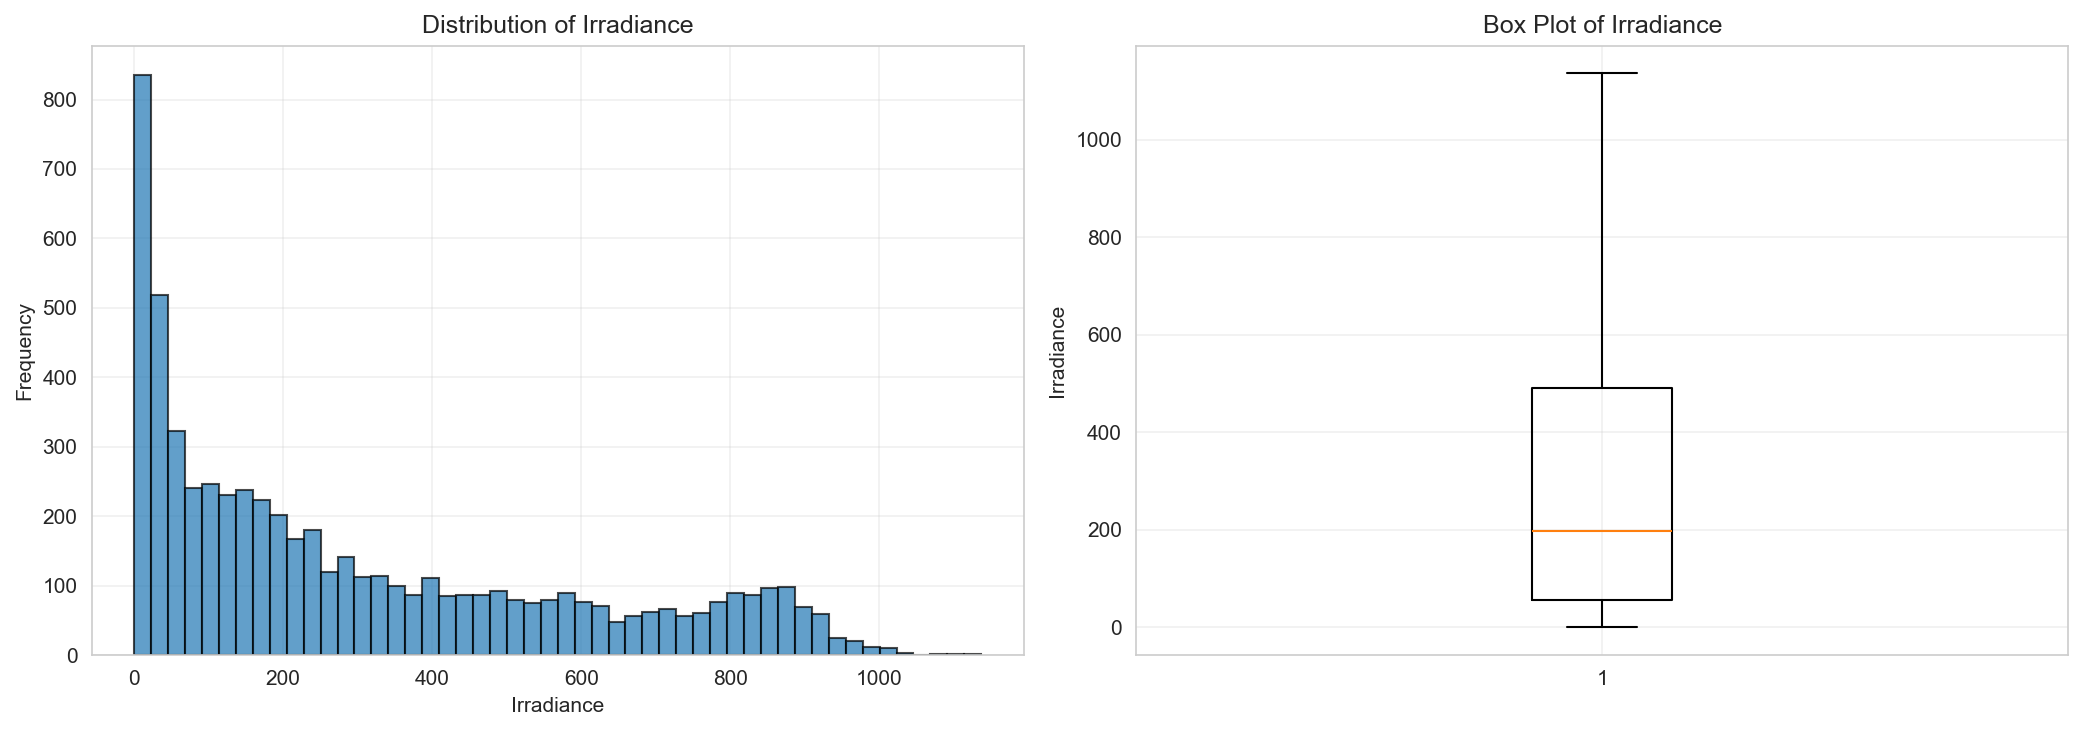
\includegraphics[width=1.1\textwidth]{../figures/eda_target_distribution.png}
    \caption{Distribúcia cieľovej premennej Irradiance}
    \label{fig:target_distribution}
\end{figure}

\textbf{Pozorovania:}
\begin{itemize}
    \item Distribúcia je pravostranná (right-skewed)
    \item Veľa vzoriek s~nízkym žiarením (zamračené dni, nočné hodiny)
    \item Menší počet vzoriek s~vysokým žiarením (jasné slnečné dni)
\end{itemize}

\clearpage

\subsection{Distribúcia žiarenia podľa mesiacov}

\begin{figure}[H]
    \centering
    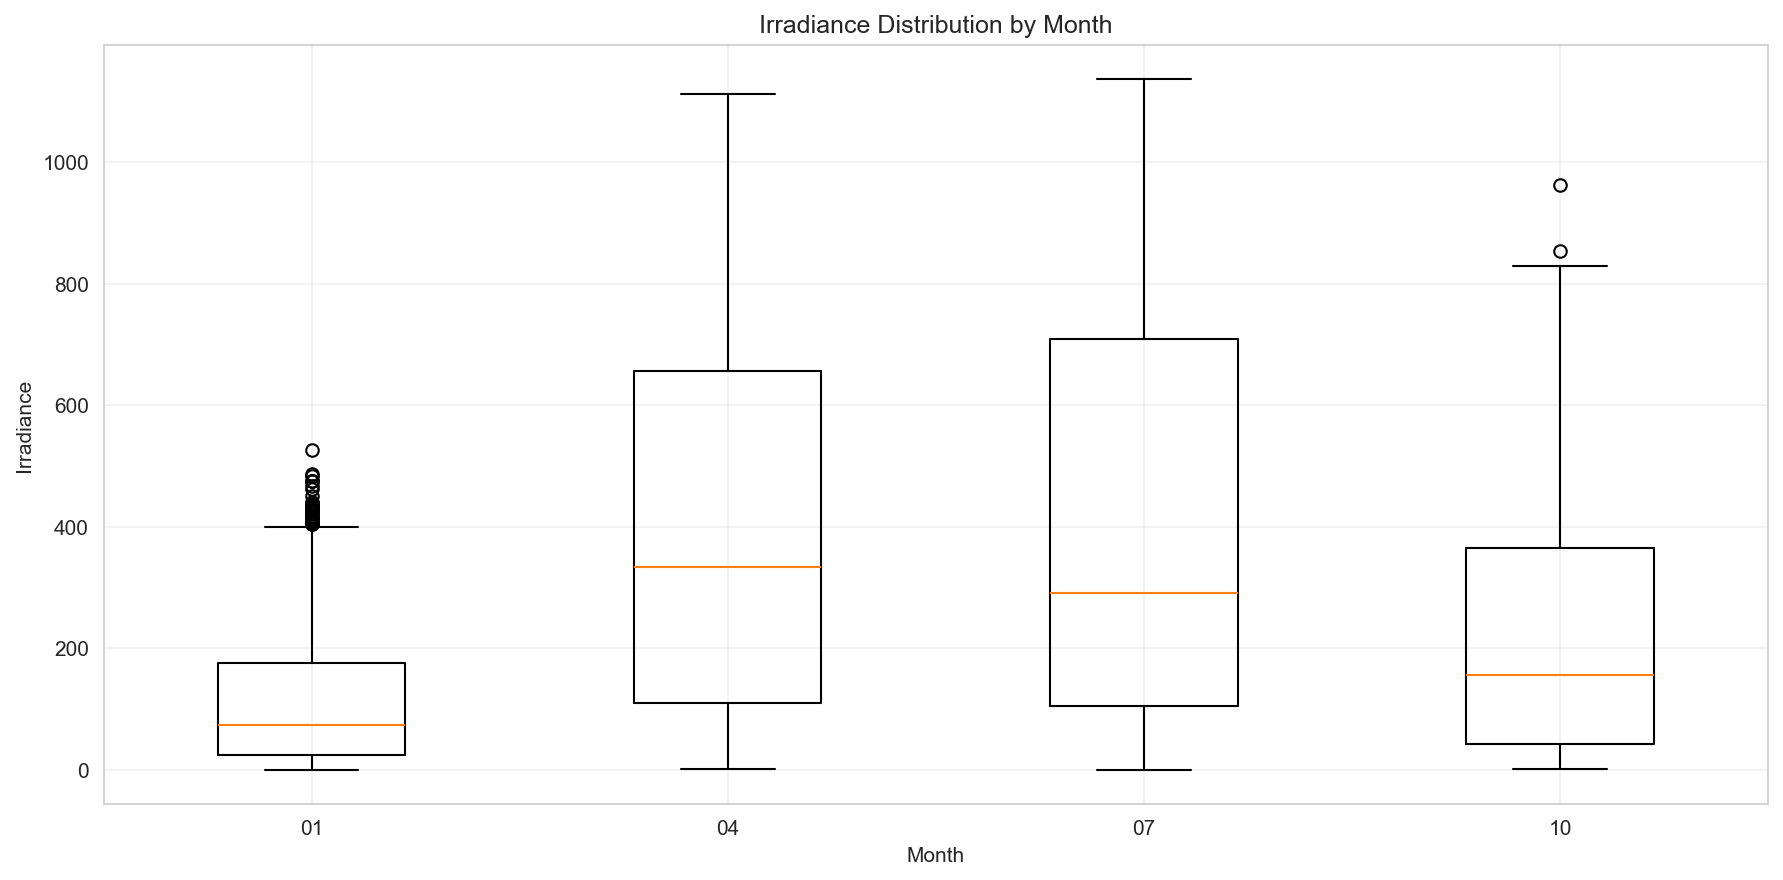
\includegraphics[width=1.1\textwidth]{../figures/eda_monthly_distribution.png}
    \caption{Distribúcia slnečného žiarenia podľa mesiacov}
    \label{fig:monthly_distribution}
\end{figure}

\textbf{Interpretácia:}
\begin{itemize}
    \item \textbf{Júl (07)}: Najvyššie priemerné žiarenie -- letné obdobie
    \item \textbf{Január (01)}: Najnižšie priemerné žiarenie -- zimné obdobie
    \item Apríl a~Október majú podobné stredné hodnoty
\end{itemize}

\clearpage

\subsection{Ukážky obrázkov}

\subsubsection{Náhodné vzorky obrázkov}

\begin{figure}[H]
    \centering
    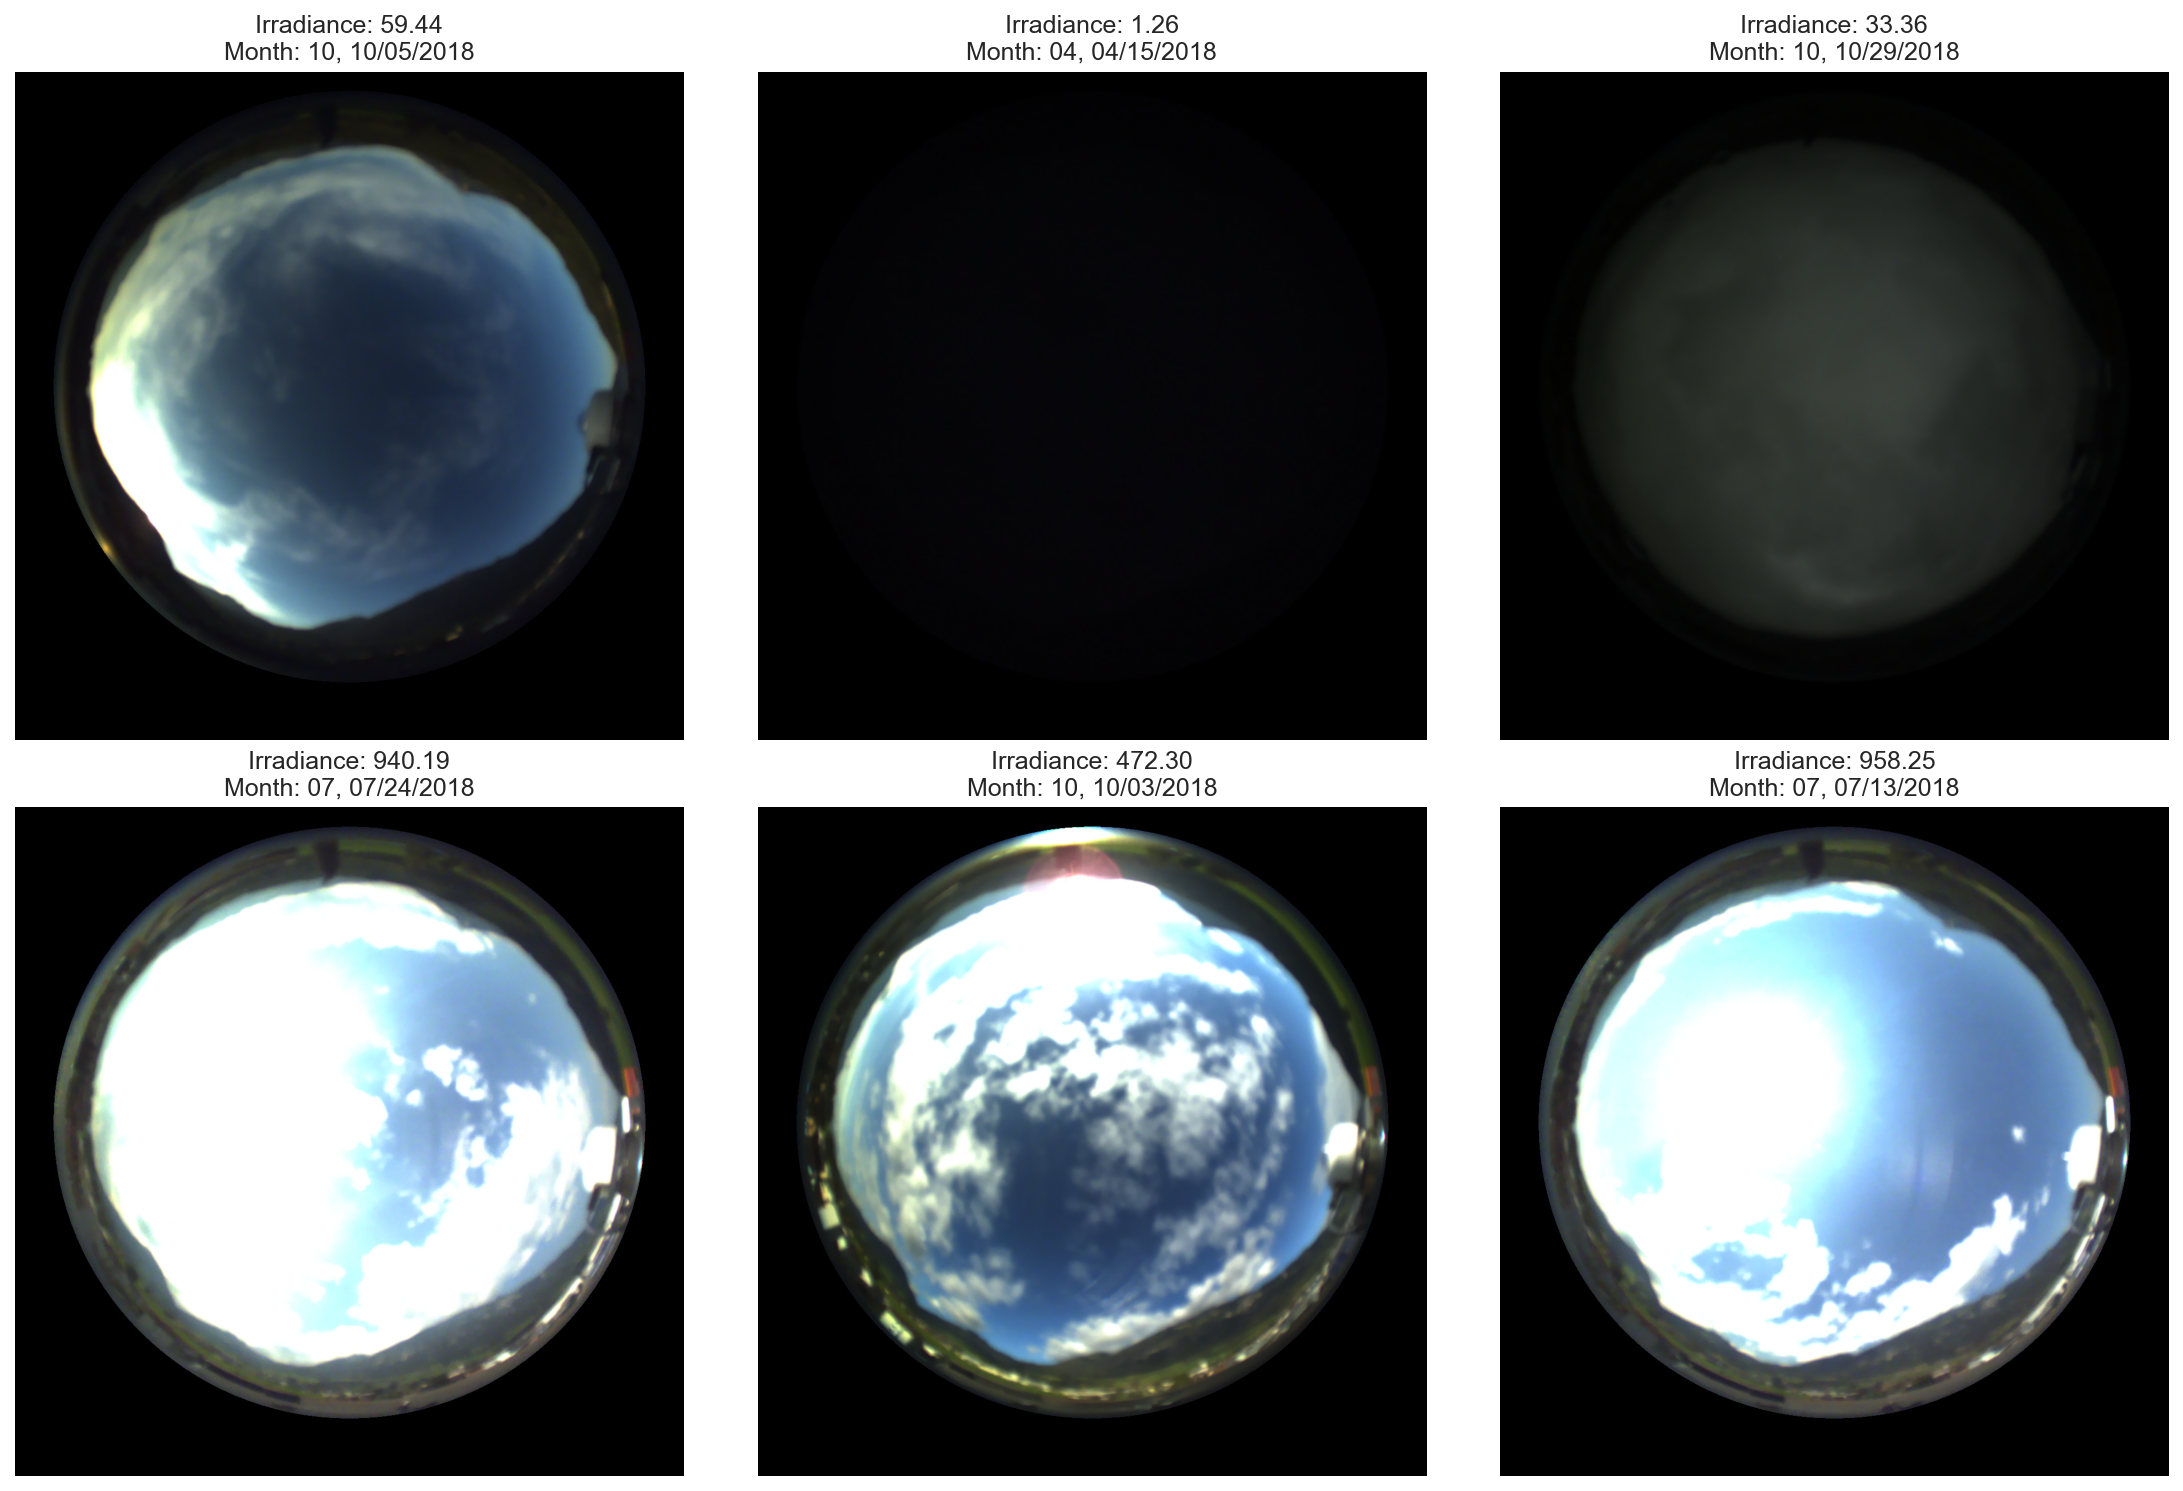
\includegraphics[width=1.1\textwidth]{../figures/eda_sample_images.png}
    \caption{Náhodné vzorky obrázkov oblohy s~hodnotami Irradiance}
    \label{fig:sample_images}
\end{figure}

\subsubsection{Obrázky s~nízkym a~vysokým žiarením}

\begin{figure}[H]
    \centering
    \begin{subfigure}[b]{0.9\textwidth}
        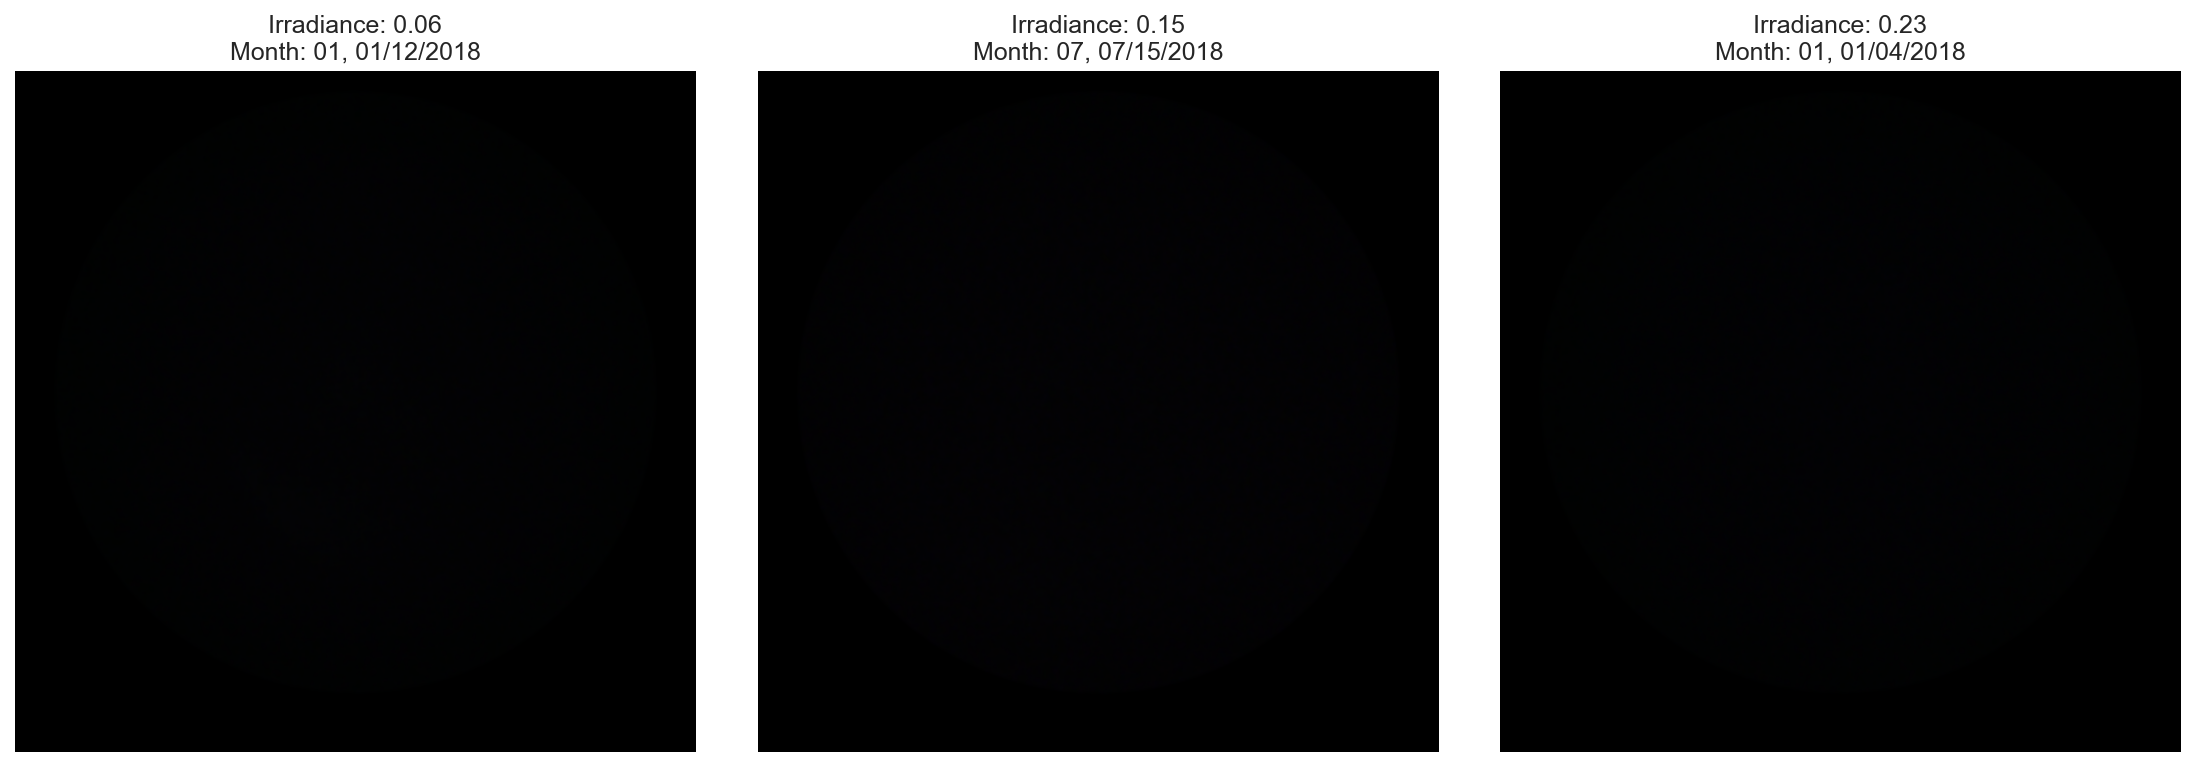
\includegraphics[width=\textwidth]{../figures/eda_low_irradiance_samples.png}
        \caption{Obrázky s~najnižším žiarením}
    \end{subfigure}
    \hfill
    \begin{subfigure}[b]{0.9\textwidth}
        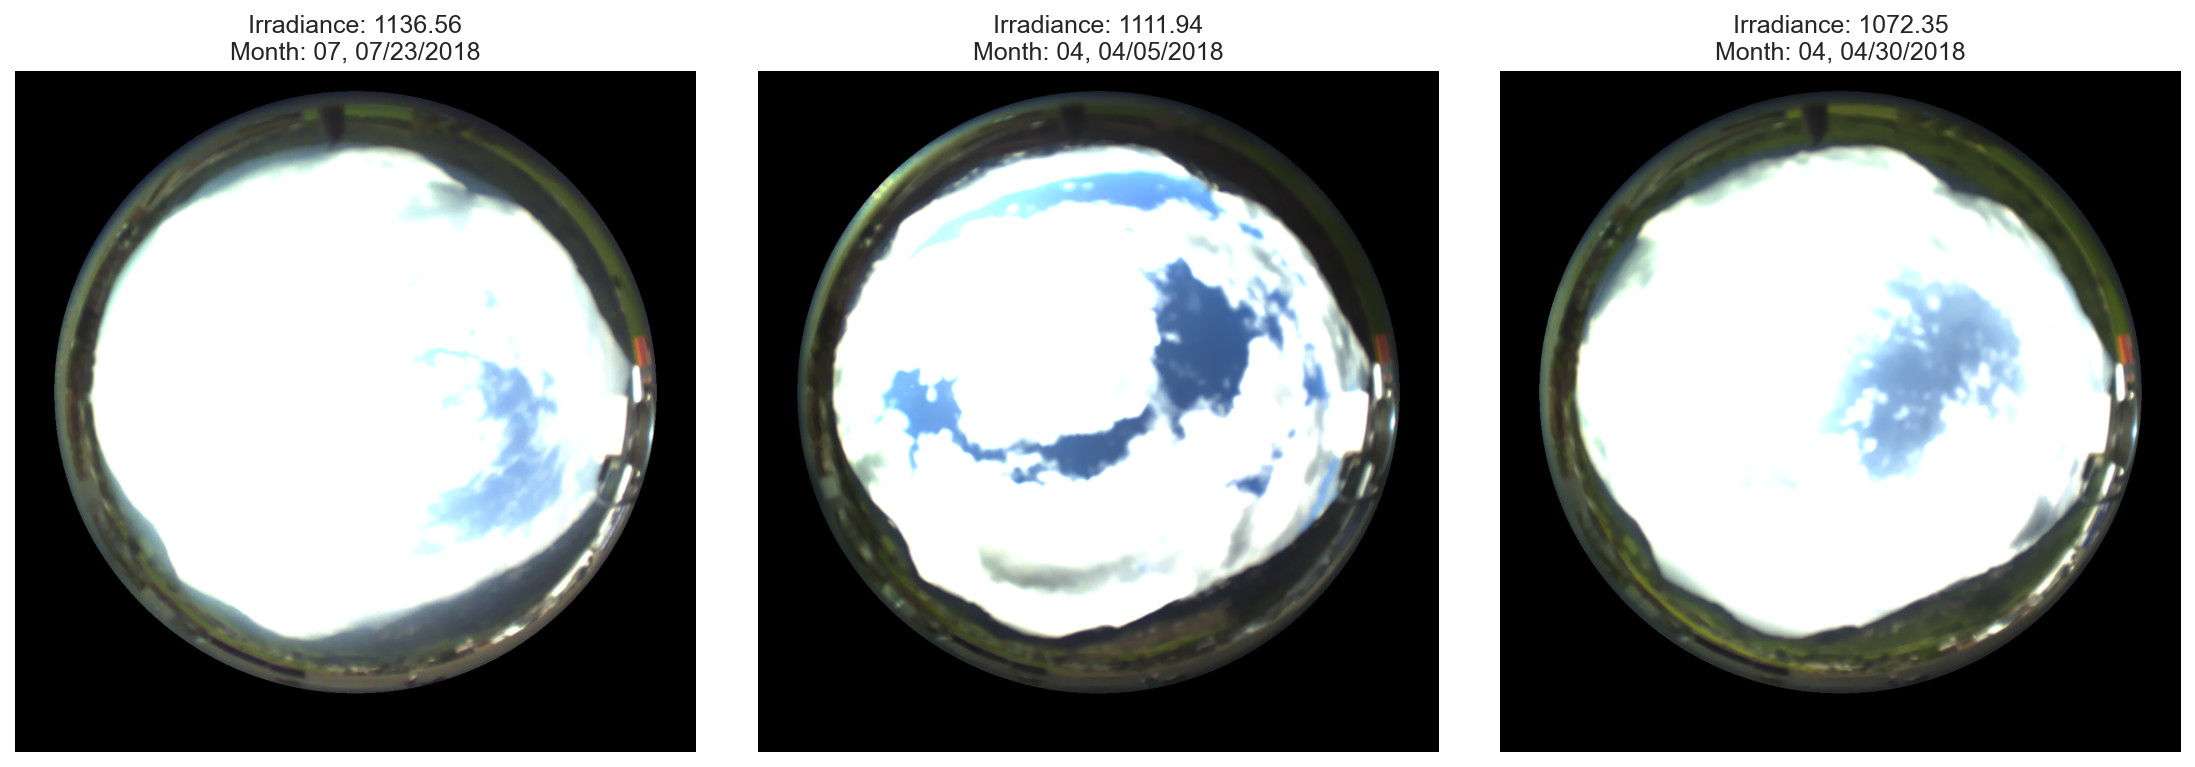
\includegraphics[width=\textwidth]{../figures/eda_high_irradiance_samples.png}
        \caption{Obrázky s~najvyšším žiarením}
    \end{subfigure}
    \caption{Porovnanie obrázkov s~extrémnym žiarením}
    \label{fig:extreme_irradiance}
\end{figure}

\textbf{Pozorovania:}
\begin{itemize}
    \item Nízke žiarenie: tmavá obloha, husté mraky, nočné/večerné hodiny
    \item Vysoké žiarenie: jasná modrá obloha, priame slnečné svetlo
\end{itemize}

\clearpage

\subsection{Korelačná analýza}

Analyzovali sme 15 numerických premenných a~ich korelácie s~cieľovou premennou Irradiance.

\begin{figure}[H]
    \centering
    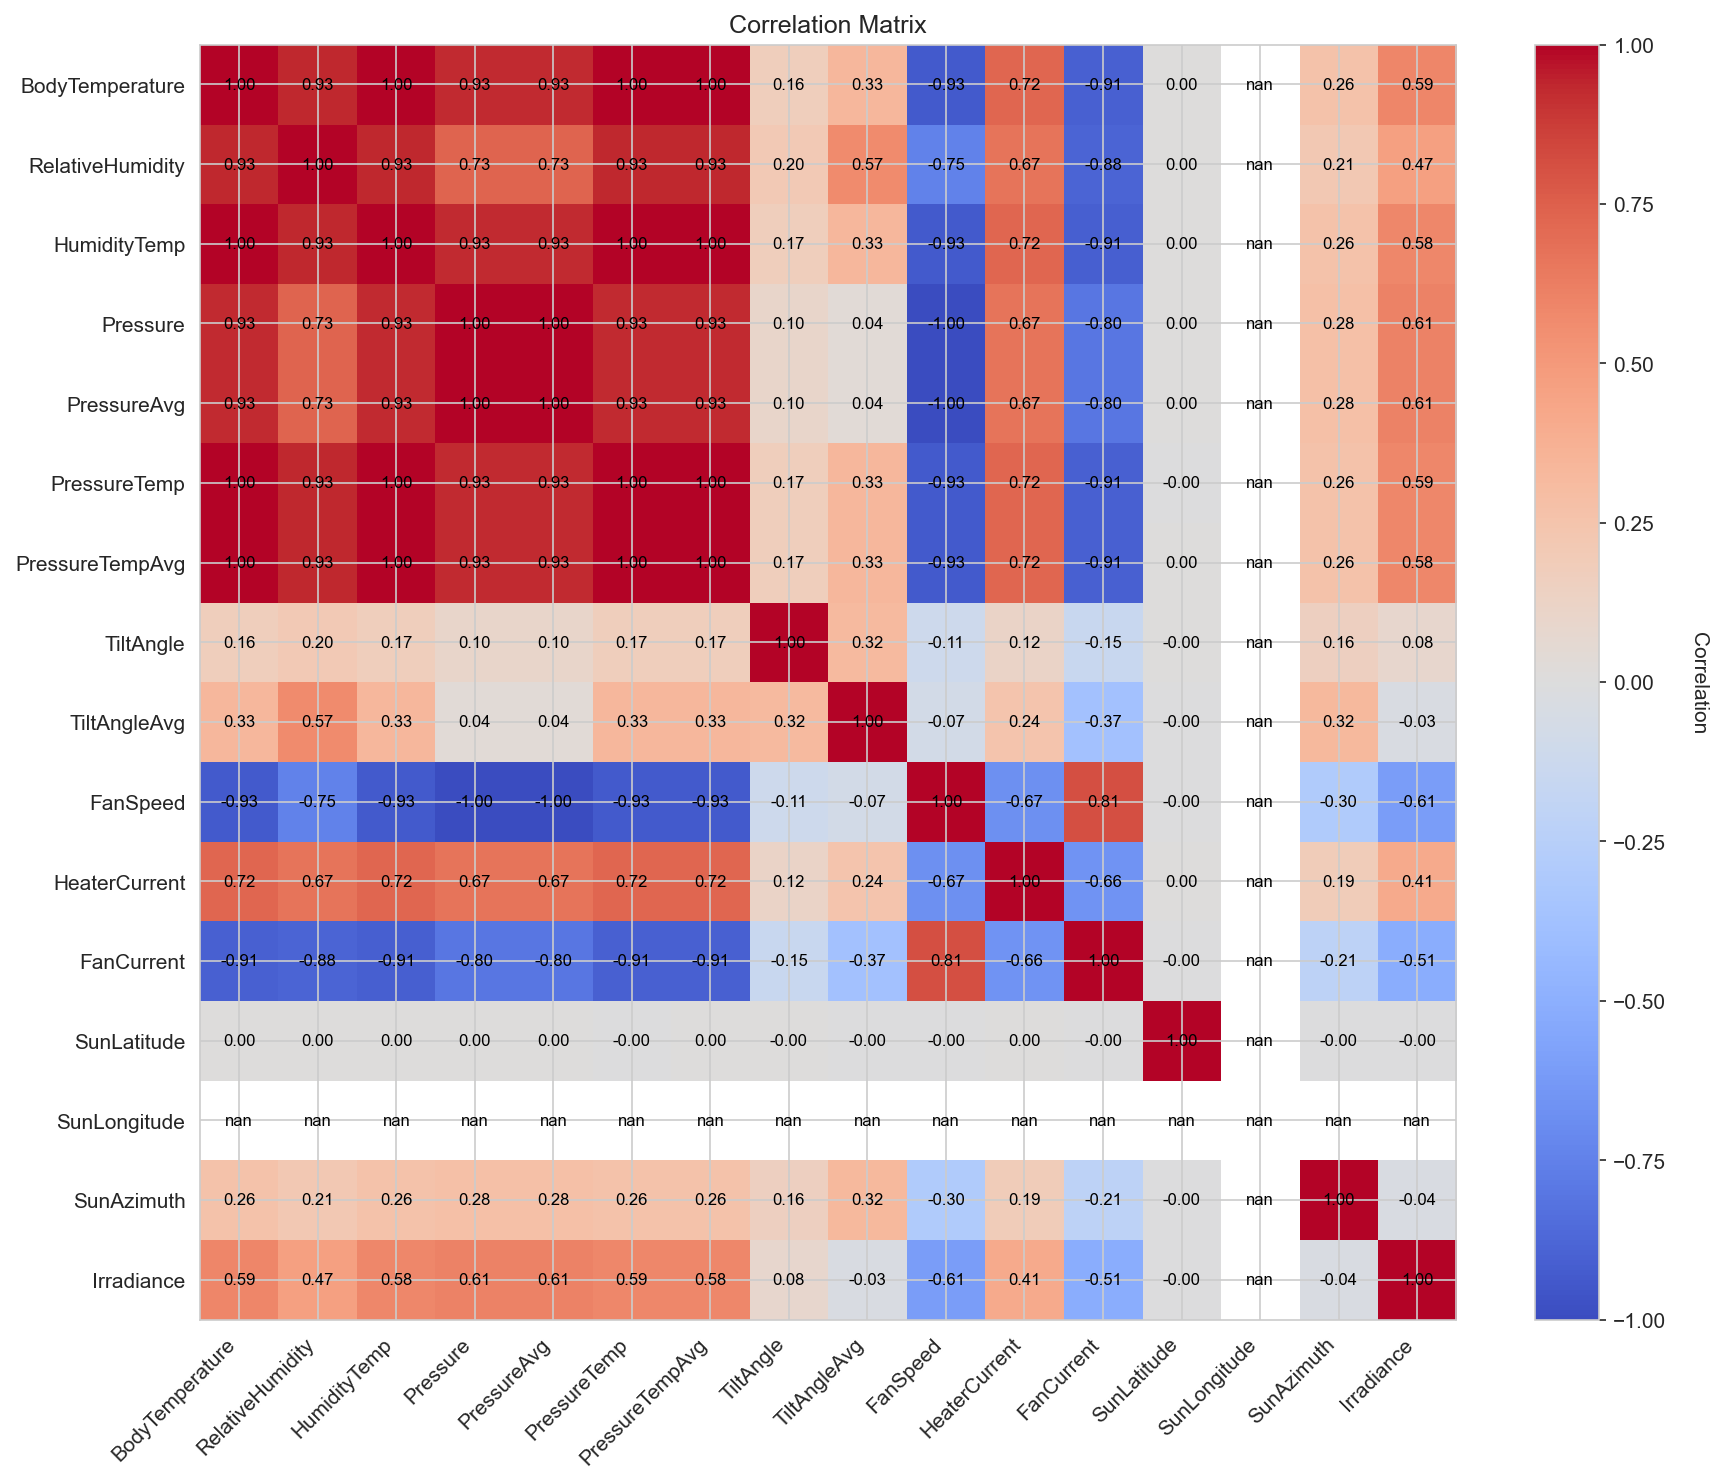
\includegraphics[width=1.12\textwidth]{../figures/eda_correlation_matrix.png}
    \caption{Korelačná matica numerických premenných}
    \label{fig:correlation_matrix}
\end{figure}

\subsubsection{Top 10 korelácií s~Irradiance}

\begin{table}[H]
\centering
\begin{tabular}{lr}
\toprule
\textbf{Premenná} & \textbf{Korelácia} \\
\midrule
Pressure & +0.6085 \\
PressureAvg & +0.6079 \\
FanSpeed & -0.6060 \\
BodyTemperature & +0.5878 \\
PressureTemp & +0.5852 \\
PressureTempAvg & +0.5846 \\
HumidityTemp & +0.5837 \\
FanCurrent & -0.5109 \\
RelativeHumidity & +0.4684 \\
HeaterCurrent & +0.4105 \\
\bottomrule
\end{tabular}
\caption{Korelácie numerických premenných s~Irradiance}
\end{table}

\subsection{Detailná analýza top features}

\begin{figure}[H]
    \centering
    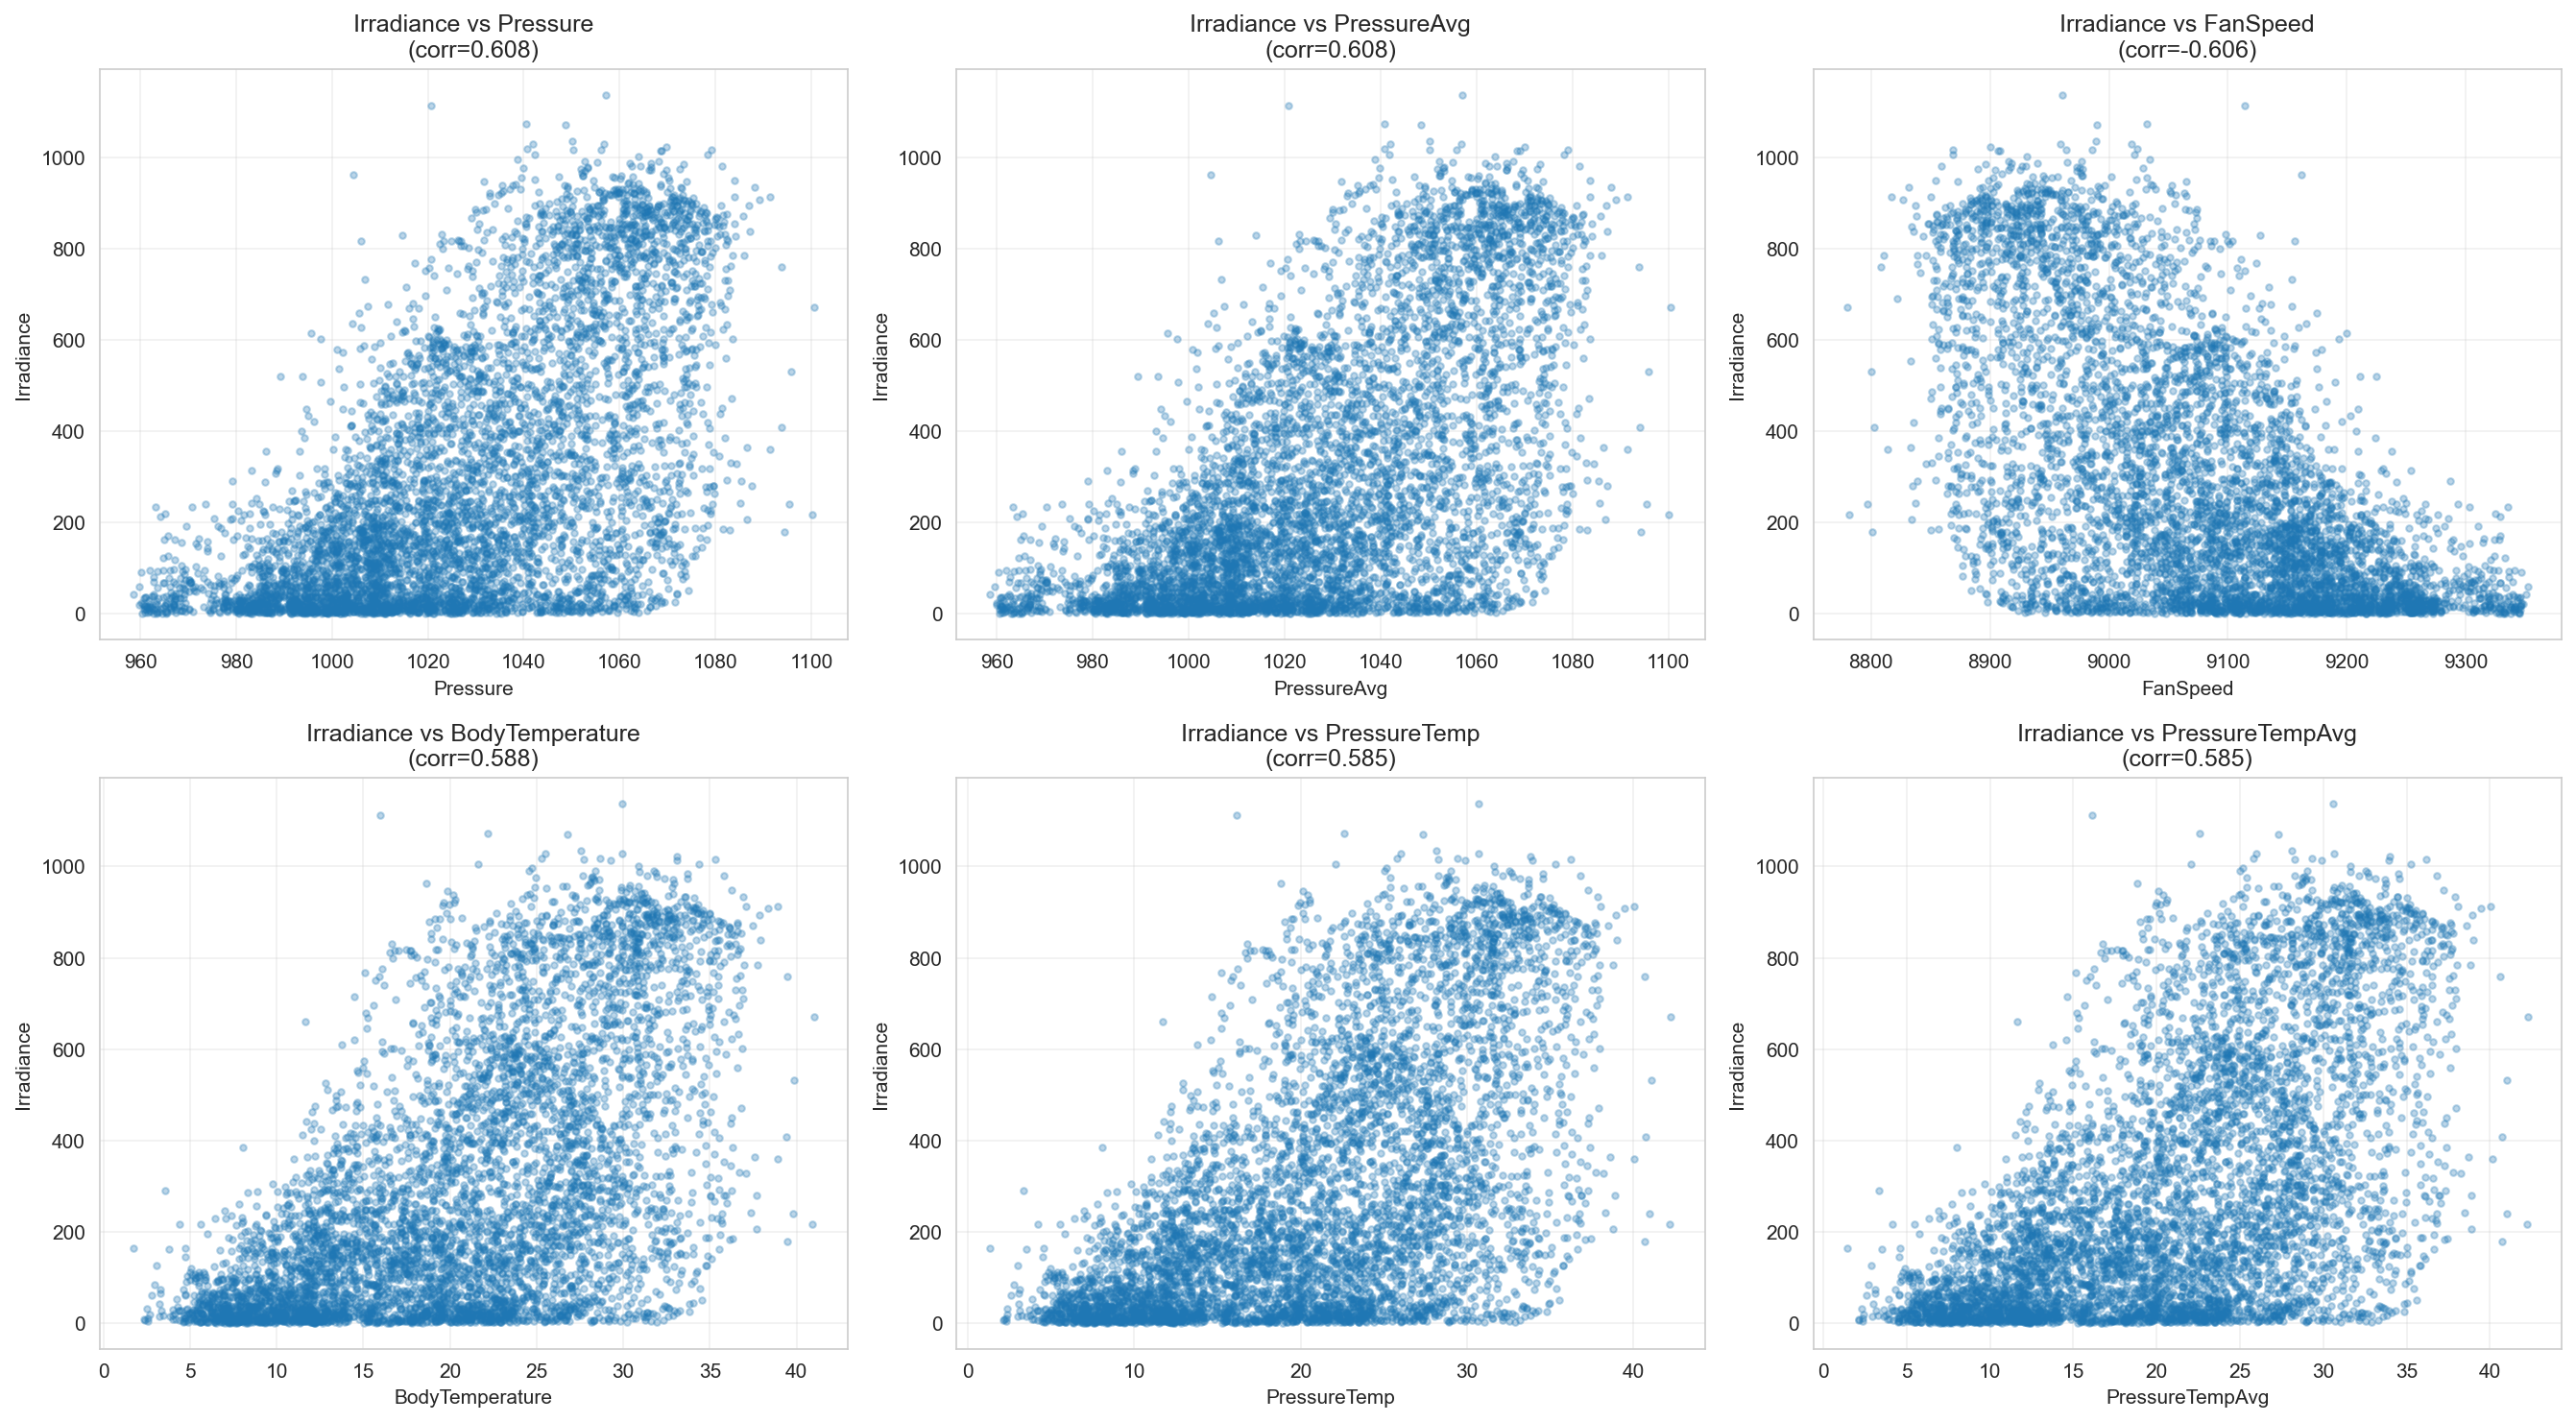
\includegraphics[width=1.12\textwidth]{../figures/eda_top_features_scatter.png}
    \caption{Scatter ploty top 6 korelovaných premenných vs Irradiance}
    \label{fig:top_features_scatter}
\end{figure}

\textbf{Interpretácia:}
\begin{itemize}
    \item Pressure a~BodyTemperature majú pozitívny lineárny vzťah so žiarením
    \item FanSpeed má negatívnu koreláciu -- ventilátor sa zapína pri vyššom žiarení
\end{itemize}

\clearpage

\subsection{Rozdelenie dát}

Dataset bol rozdelený na trénovaciu, validačnú a~testovaciu množinu:

\begin{table}[H]
\centering
\begin{tabular}{lrr}
\toprule
\textbf{Množina} & \textbf{Počet vzoriek} & \textbf{Podiel (\%)} \\
\midrule
Trénovacia & 4~204 & 70.0 \\
Validačná & 901 & 15.0 \\
Testovacia & 902 & 15.0 \\
\midrule
\textbf{Celkom} & \textbf{6~007} & \textbf{100.0} \\
\bottomrule
\end{tabular}
\caption{Rozdelenie datasetu}
\end{table}

\begin{figure}[H]
    \centering
    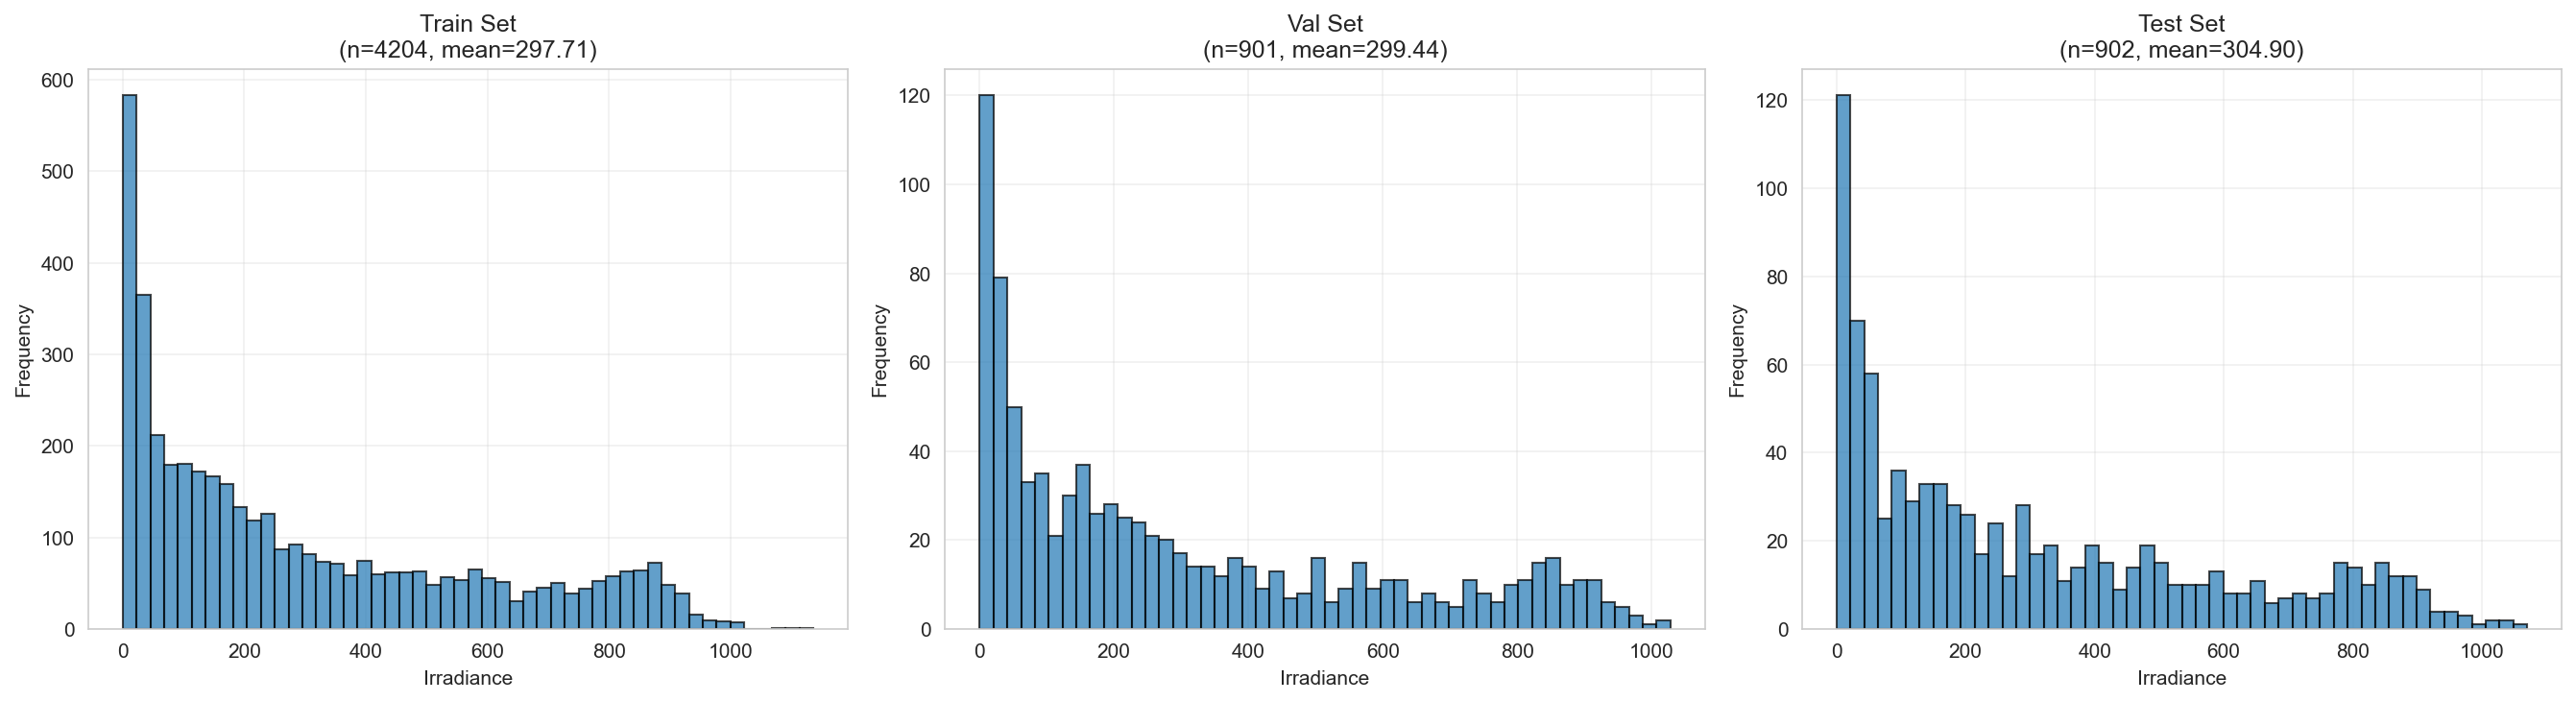
\includegraphics[width=1.1\textwidth]{../figures/eda_split_distributions.png}
    \caption{Distribúcia Irradiance v~jednotlivých splitoch}
    \label{fig:split_distributions}
\end{figure}

\textbf{Kontrola:} Distribúcie sú konzistentné naprieč všetkými splitmi.

\clearpage

\section{Konvolučné neurónové siete (CNN)}

\subsection{Architektúra CNN}

Navrhli sme vlastnú konvolučnú neurónovú sieť pre regresiu slnečného žiarenia:

\begin{table}[H]
\centering
\begin{tabular}{lrr}
\toprule
\textbf{Vrstva} & \textbf{Parametre} & \textbf{Popis} \\
\midrule
Input & 3×128×128 & RGB obrázok \\
Conv Block 1 & Conv2D + BN + ReLU + MaxPool & Extrakcia nízkoúrovňových features \\
Conv Block 2 & Conv2D + BN + ReLU + MaxPool & Strednoúrovňové features \\
Conv Block 3 & Conv2D + BN + ReLU + MaxPool & Vysokoúrovňové features \\
Flatten & -- & Prevod na 1D vektor \\
FC + Dropout & Hidden neurons + ReLU & Plne prepojené vrstvy \\
Output & 1 neuron & Predikcia Irradiance \\
\bottomrule
\end{tabular}
\caption{Architektúra CNN modelu}
\end{table}

\textbf{Pravidlá návrhu:}
\begin{itemize}
    \item Počet konvolučných kanálov > počet FC neurónov
    \item Dropout aplikovaný len na FC vrstvy
    \item Batch Normalization po každej konvolúcii
\end{itemize}

\subsection{Konfigurácie hyperparametrov}

Testovali sme 5 rôznych konfigurácií:

\begin{table}[H]
\centering
\small
\begin{tabular}{lrrrrr}
\toprule
\textbf{Konfigurácia} & \textbf{Conv} & \textbf{FC} & \textbf{Dropout} & \textbf{WD} & \textbf{Epochs} \\
\midrule
1: Základná & [16,32,64] & [32,16] & 0.65 & 0.03 & 8 \\
2: Hlbšia sieť & [16,32,64,128] & [64,32] & 0.65 & 0.03 & 8 \\
3: Vyšší dropout & [16,32,64] & [32,16] & 0.70 & 0.03 & 8 \\
4: Väčší weight decay & [16,32,64] & [32,16] & 0.65 & 0.10 & 8 \\
5: Širšia sieť & [24,48,96] & [48,24] & 0.65 & 0.04 & 8 \\
\bottomrule
\end{tabular}
\caption{Konfigurácie CNN modelov}
\end{table}

\clearpage

\subsection{Výsledky trénovania CNN}

\begin{table}[H]
\centering
\small
\begin{tabular}{lrrrrrr}
\toprule
\textbf{Konfigurácia} & \textbf{Params} & \textbf{Train R²} & \textbf{Test R²} & \textbf{Test RMSE} & \textbf{Test MAE} \\
\midrule
1: Základná & 173~457 & 0.9292 & 0.9275 & 76.49 & 53.09 \\
2: Hlbšia sieť & 698~065 & 0.9729 & 0.9722 & 47.39 & 30.14 \\
3: Vyšší dropout & 173~457 & 0.9346 & 0.9341 & 72.90 & 50.94 \\
4: Väčší weight decay & 173~457 & 0.9243 & 0.9231 & 78.75 & 53.70 \\
\textbf{5: Širšia sieť} & \textbf{389~401} & \textbf{0.9737} & \textbf{0.9744} & \textbf{45.43} & \textbf{31.37} \\
\bottomrule
\end{tabular}
\caption{Výsledky všetkých CNN konfigurácií}
\end{table}

\subsubsection{Najlepšia konfigurácia}

\begin{itemize}
    \item \textbf{Konfigurácia 5: Širšia sieť}
    \item Test R²: \textbf{0.9744}
    \item Test RMSE: \textbf{45.43 W/m²}
    \item Test MAE: \textbf{31.37 W/m²}
    \item Počet parametrov: 389~401
\end{itemize}

\subsubsection{Analýza overfittingu}

\begin{table}[H]
\centering
\begin{tabular}{lrrr}
\toprule
\textbf{Konfigurácia} & \textbf{Train R²} & \textbf{Test R²} & \textbf{Rozdiel} \\
\midrule
1: Základná & 0.9292 & 0.9275 & 0.0017 \\
2: Hlbšia sieť & 0.9729 & 0.9722 & 0.0007 \\
3: Vyšší dropout & 0.9346 & 0.9341 & 0.0005 \\
4: Väčší weight decay & 0.9243 & 0.9231 & 0.0012 \\
5: Širšia sieť & 0.9737 & 0.9744 & -0.0007 \\
\bottomrule
\end{tabular}
\caption{Analýza overfittingu CNN modelov}
\end{table}

\textbf{Záver:} Žiadna konfigurácia nevykazuje významný overfitting. Konfigurácia 5 má dokonca mierne lepší výkon na teste než na tréningu.

\clearpage

\subsection{História trénovania najlepšieho modelu}

\begin{figure}[H]
    \centering
    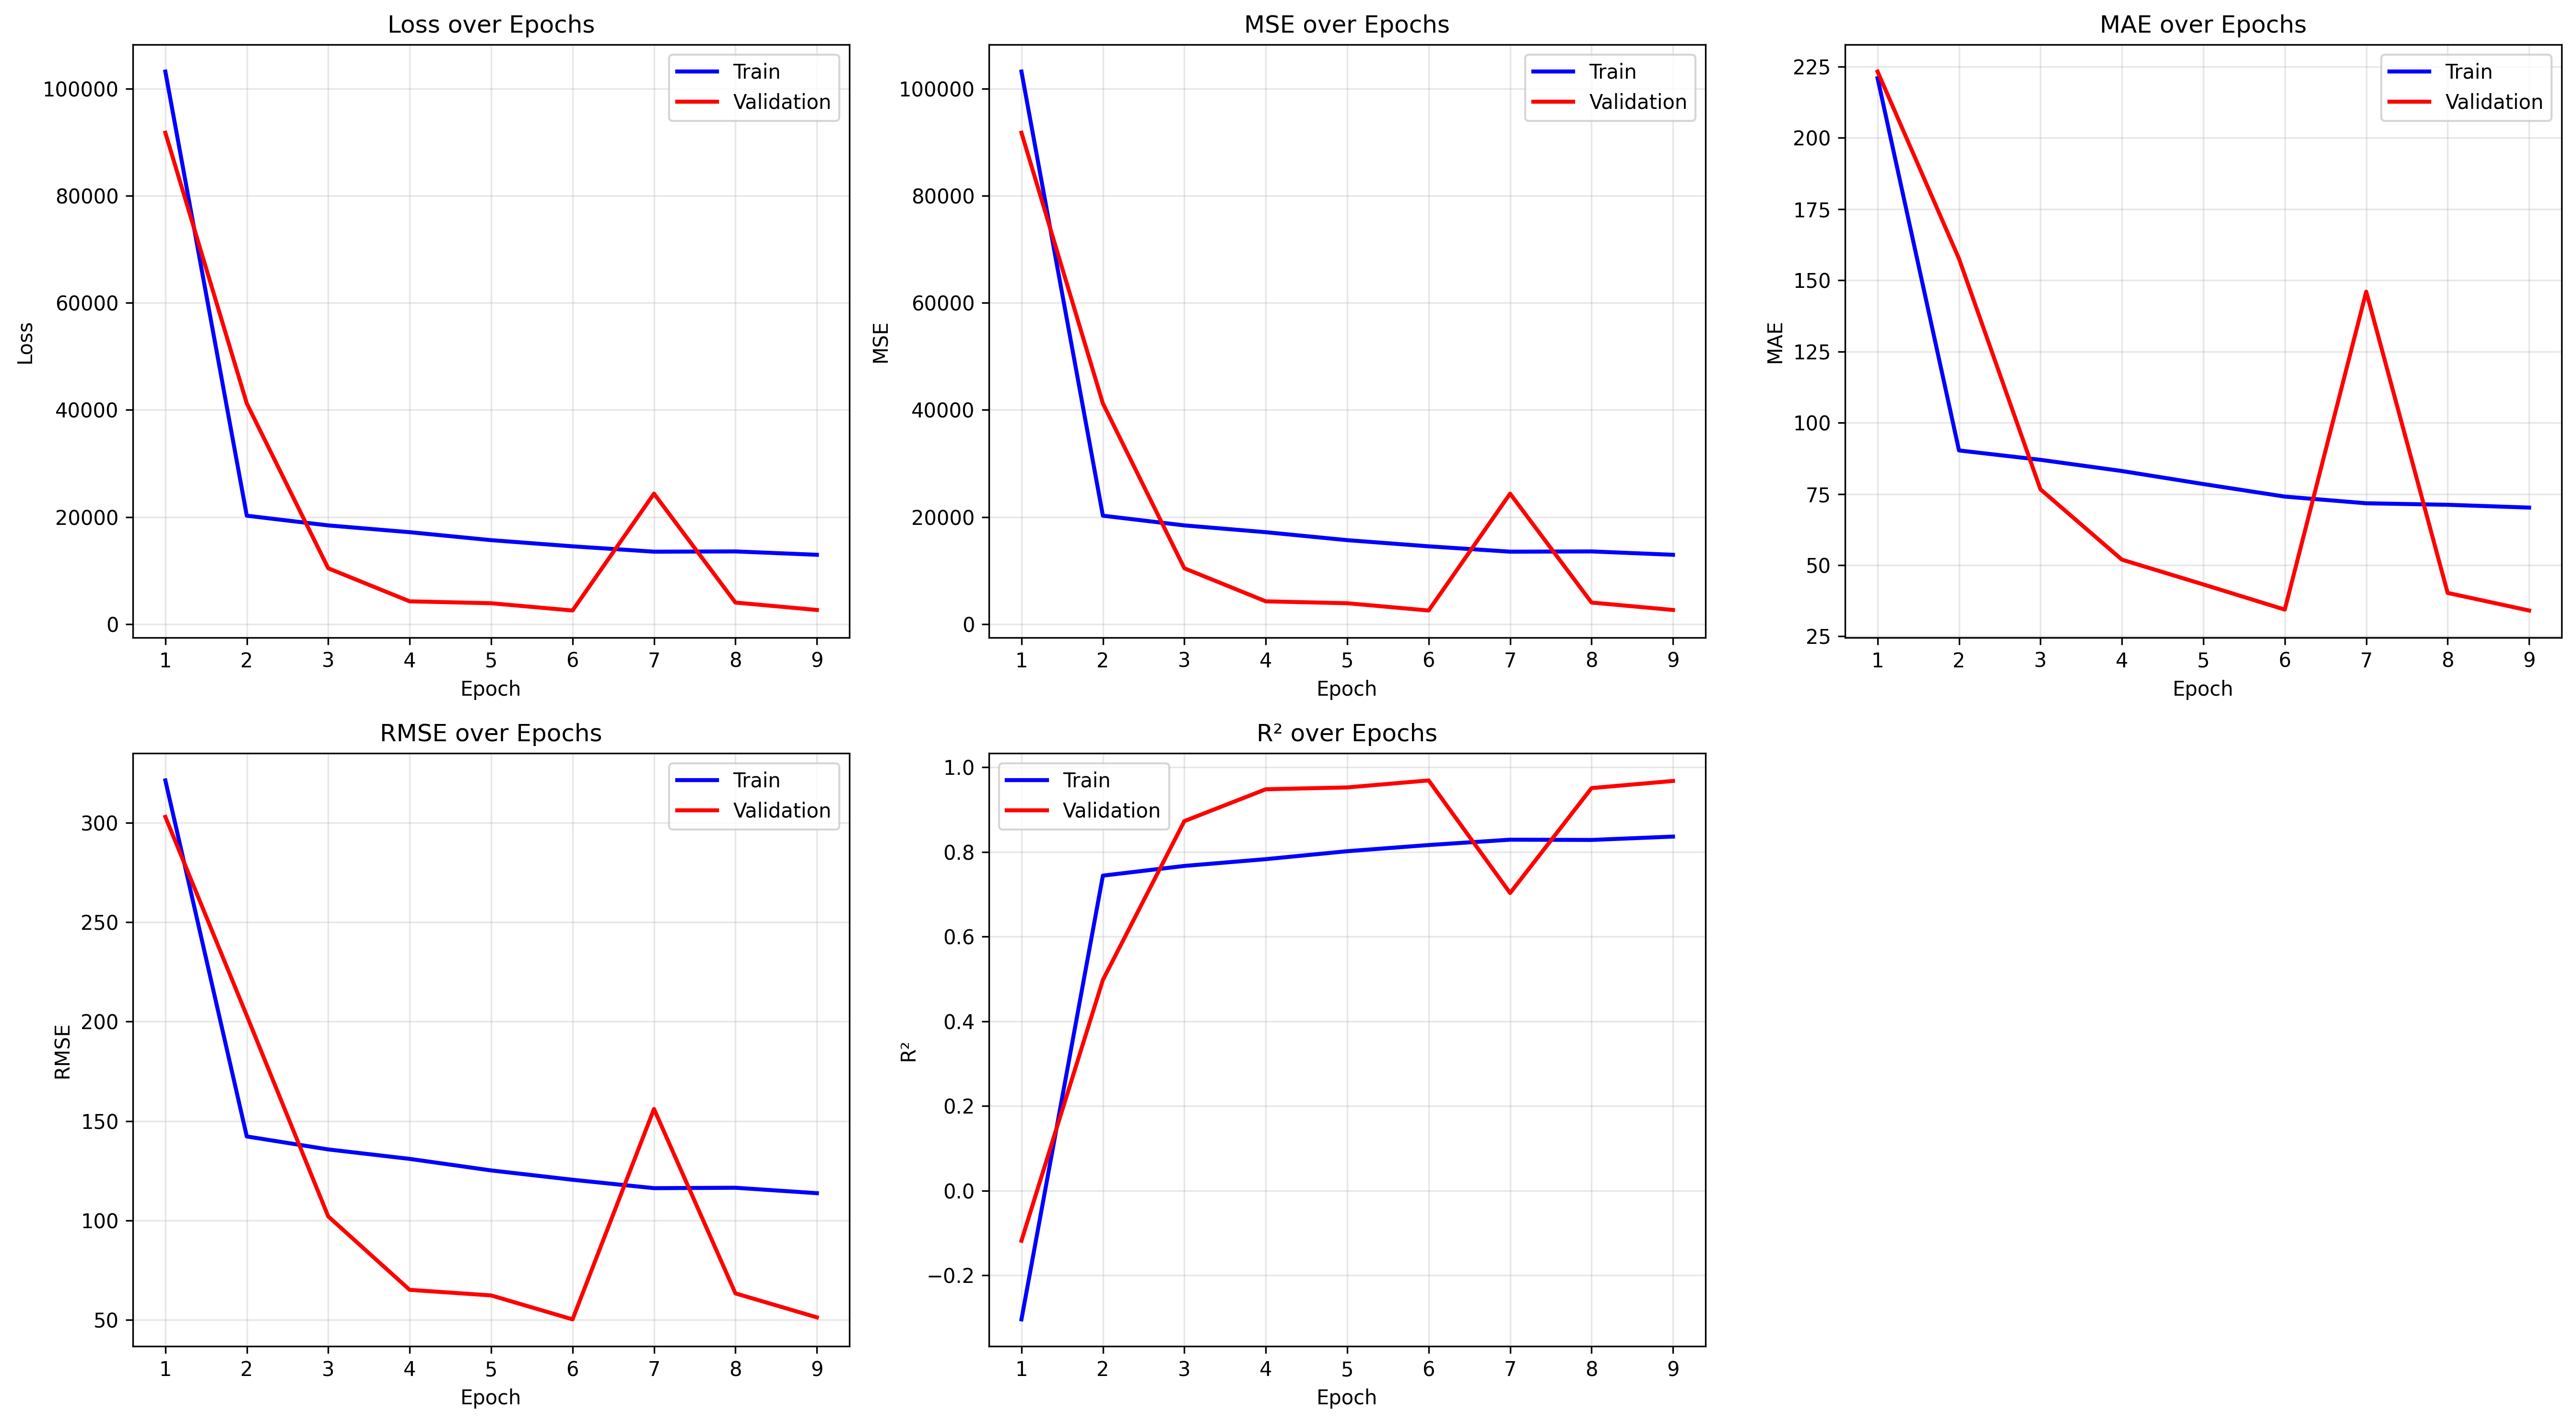
\includegraphics[width=1.1\textwidth]{../figures/training_history_config_5.png}
    \caption{História trénovania Konfigurácie 5 (Širšia sieť)}
    \label{fig:training_history}
\end{figure}

\subsection{Analýza reziduálov}

\begin{figure}[H]
    \centering
    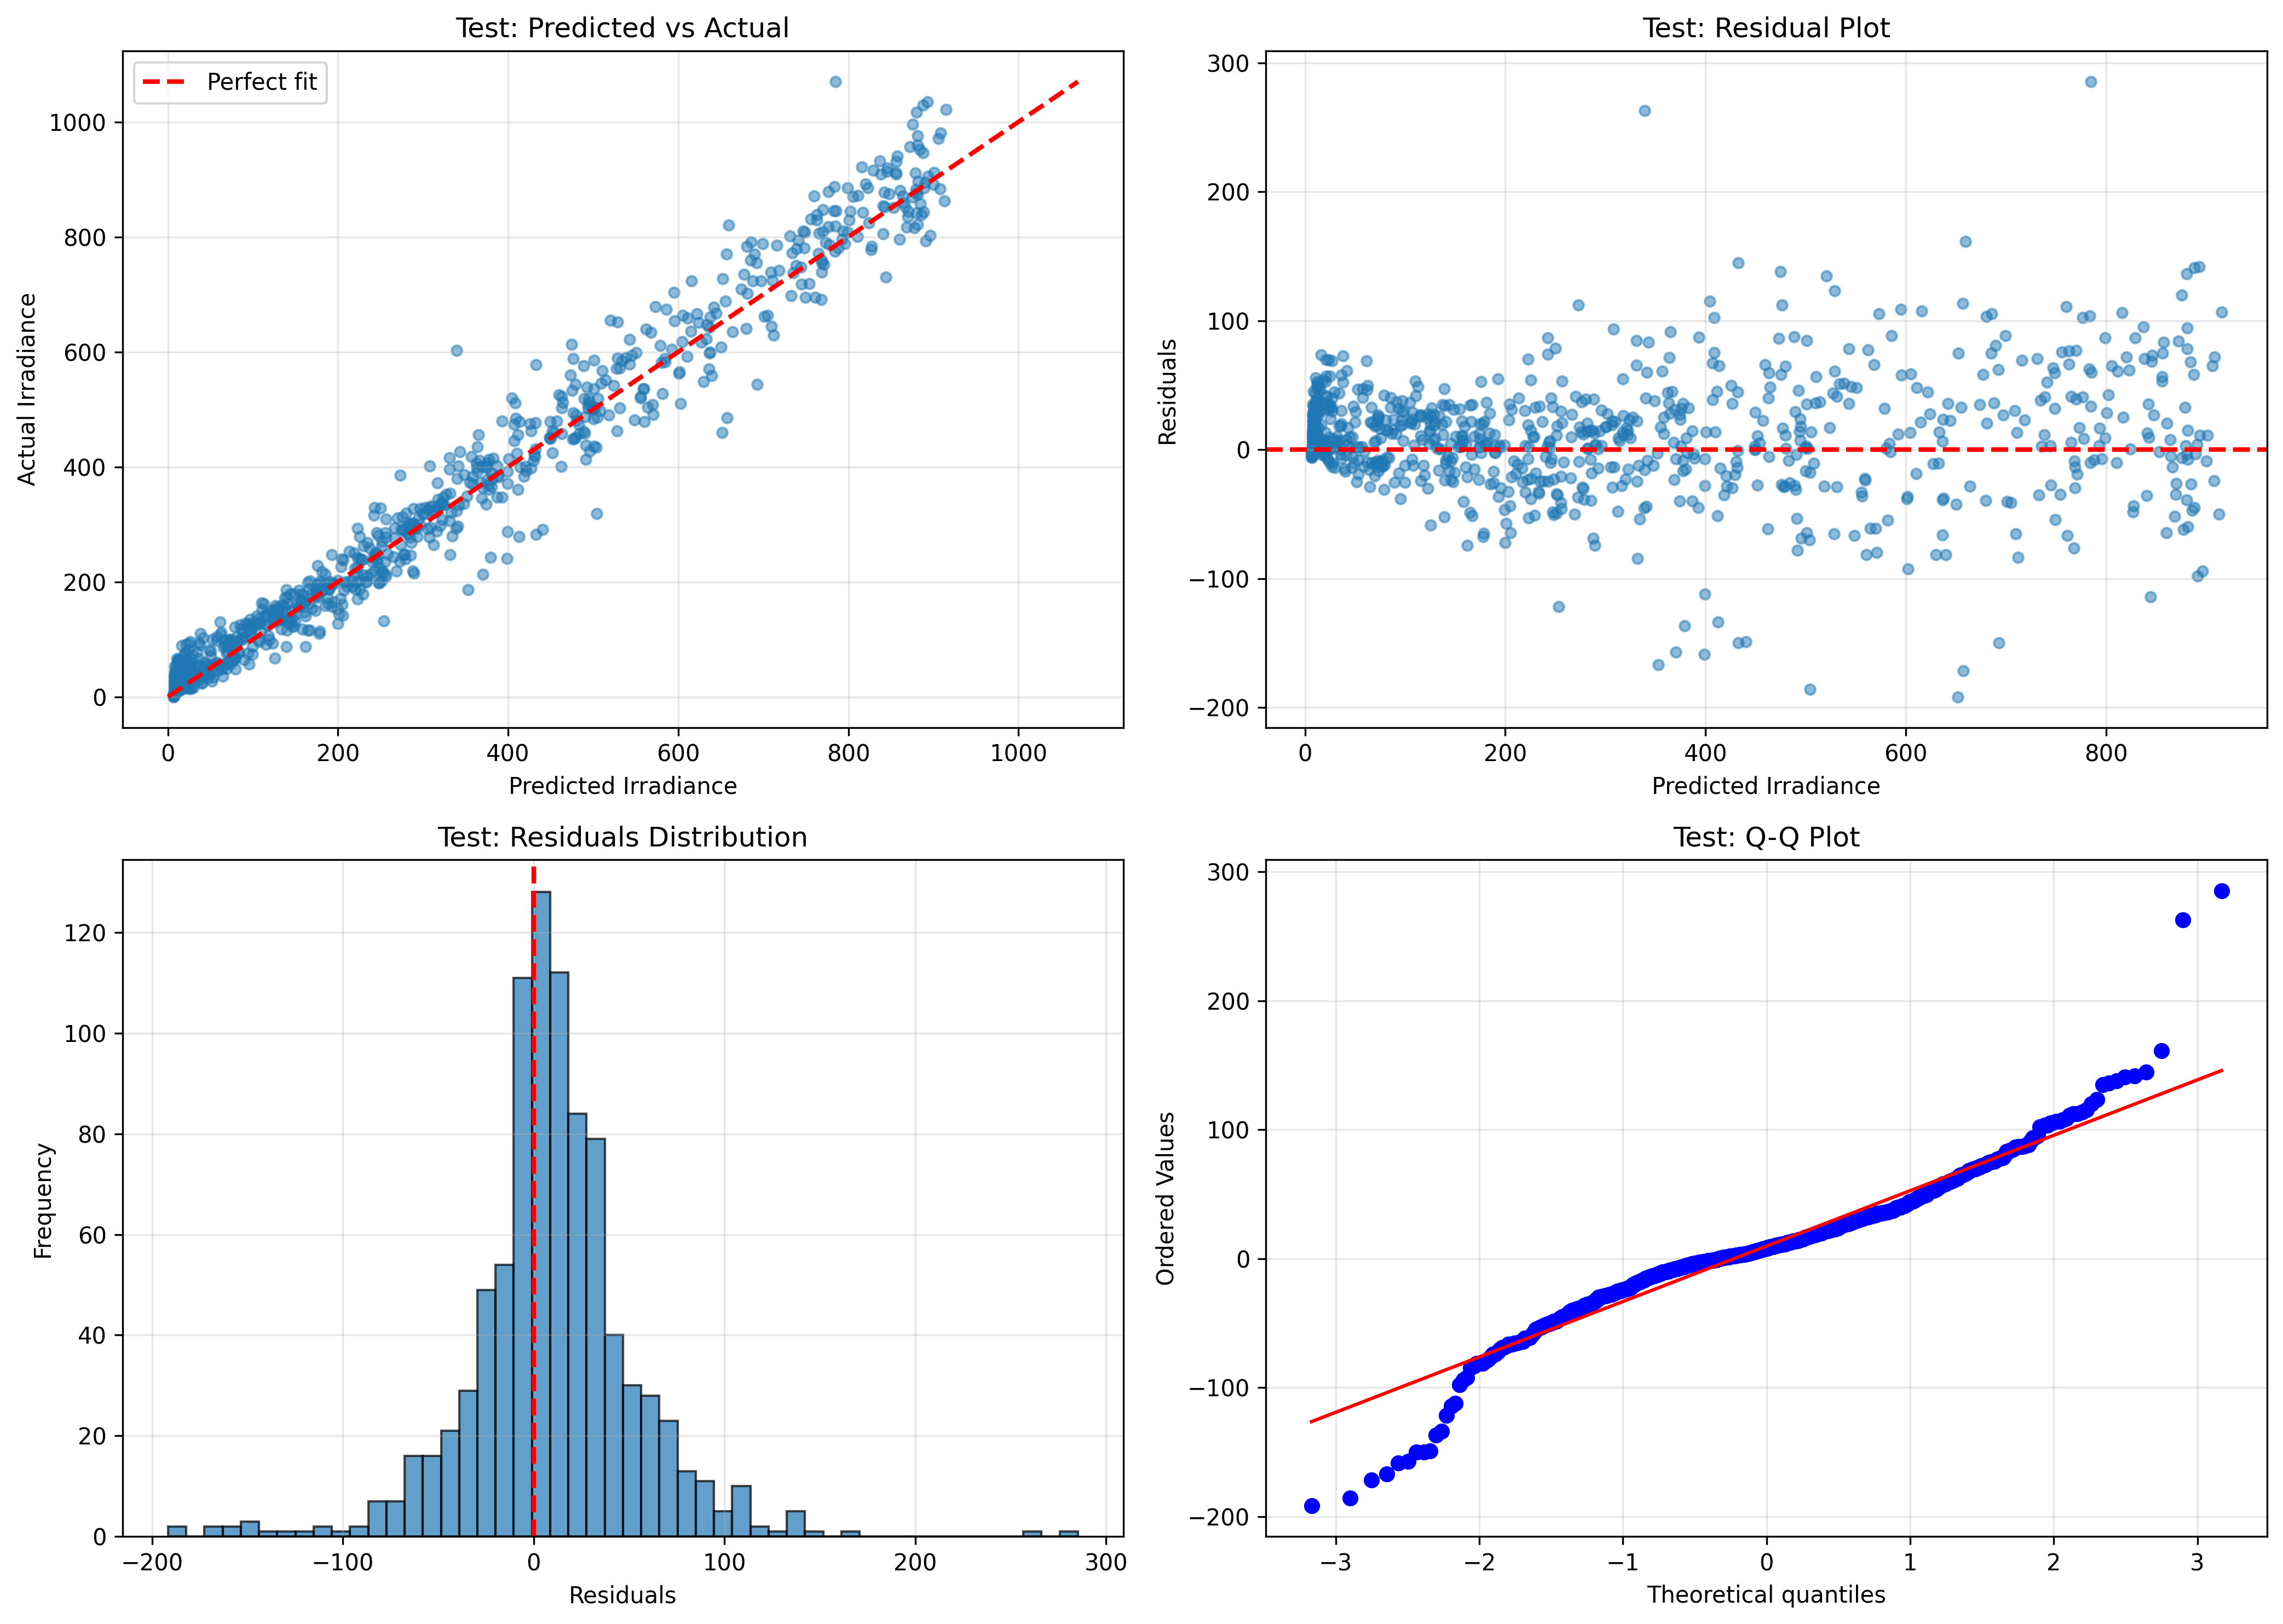
\includegraphics[width=1.1\textwidth]{../figures/residuals_config_5.png}
    \caption{Reziduálna analýza najlepšieho CNN modelu}
    \label{fig:residuals}
\end{figure}

\clearpage

\subsection{Porovnanie predikcií}

\begin{figure}[H]
    \centering
    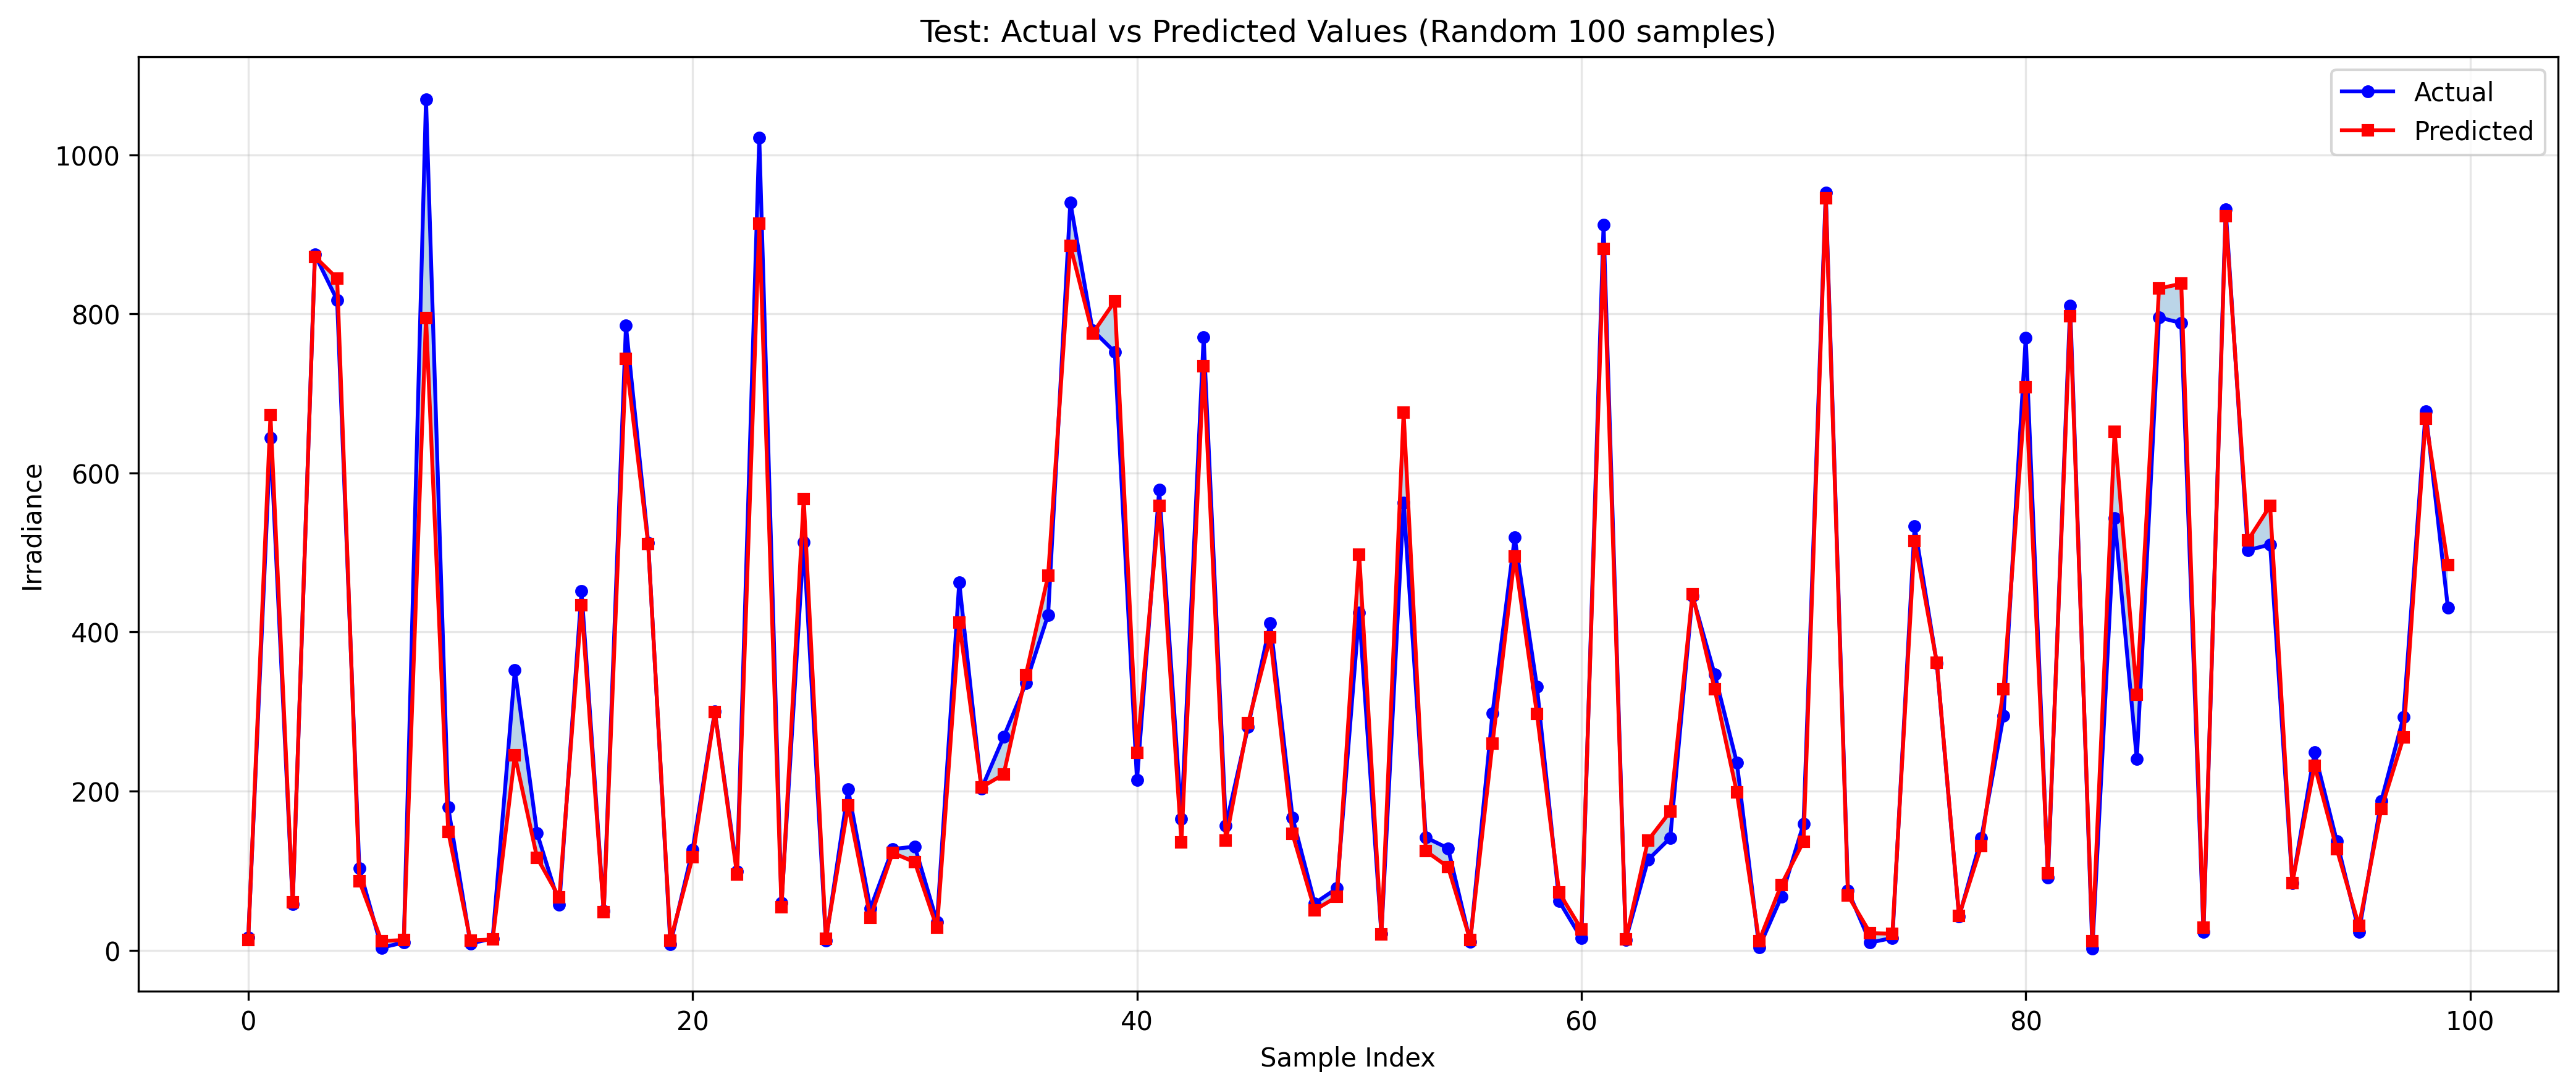
\includegraphics[width=1.1\textwidth]{../figures/predictions_comparison_config_5.png}
    \caption{Porovnanie predikcií vs. skutočných hodnôt (100 vzoriek)}
    \label{fig:predictions_comparison}
\end{figure}

\subsection{Vizualizácia konvolučných filtrov}

\begin{figure}[H]
    \centering
    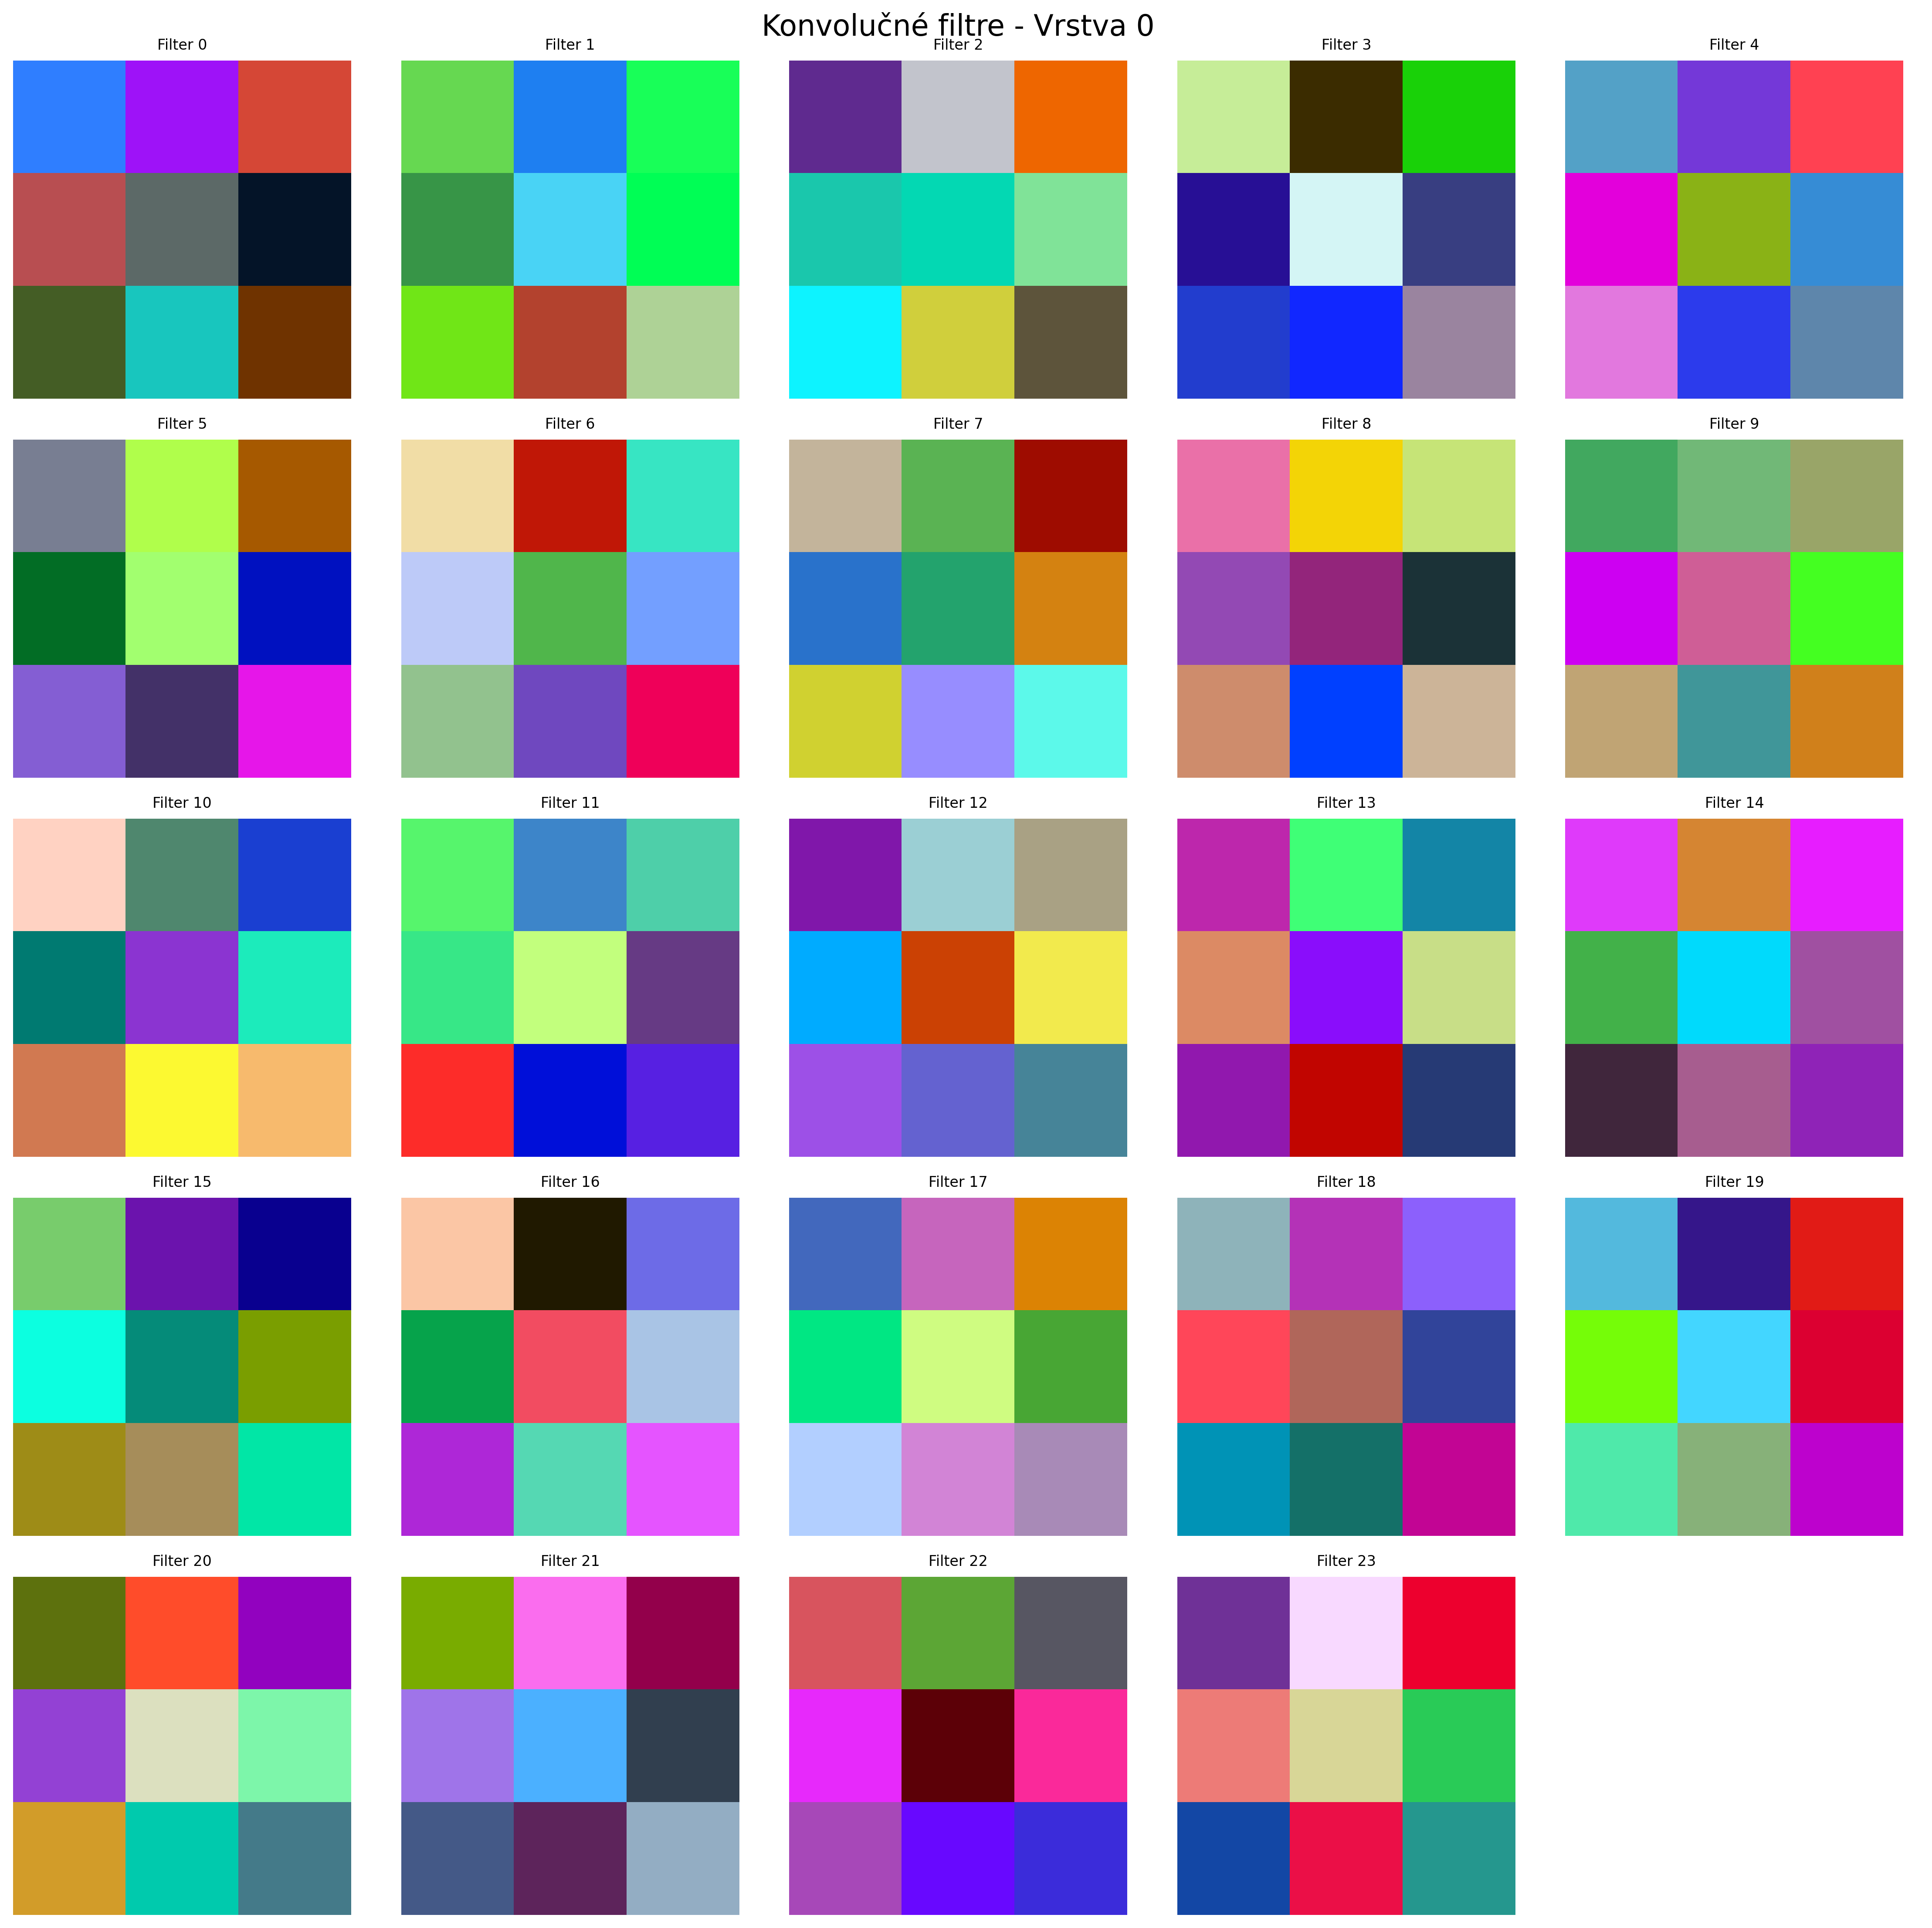
\includegraphics[width=1.1\textwidth]{../figures/conv_filters_layer_0_config_5.png}
    \caption{Filtre prvej konvolučnej vrstvy}
    \label{fig:conv_filters_layer_0}
\end{figure}

\clearpage

\begin{figure}[H]
    \centering
    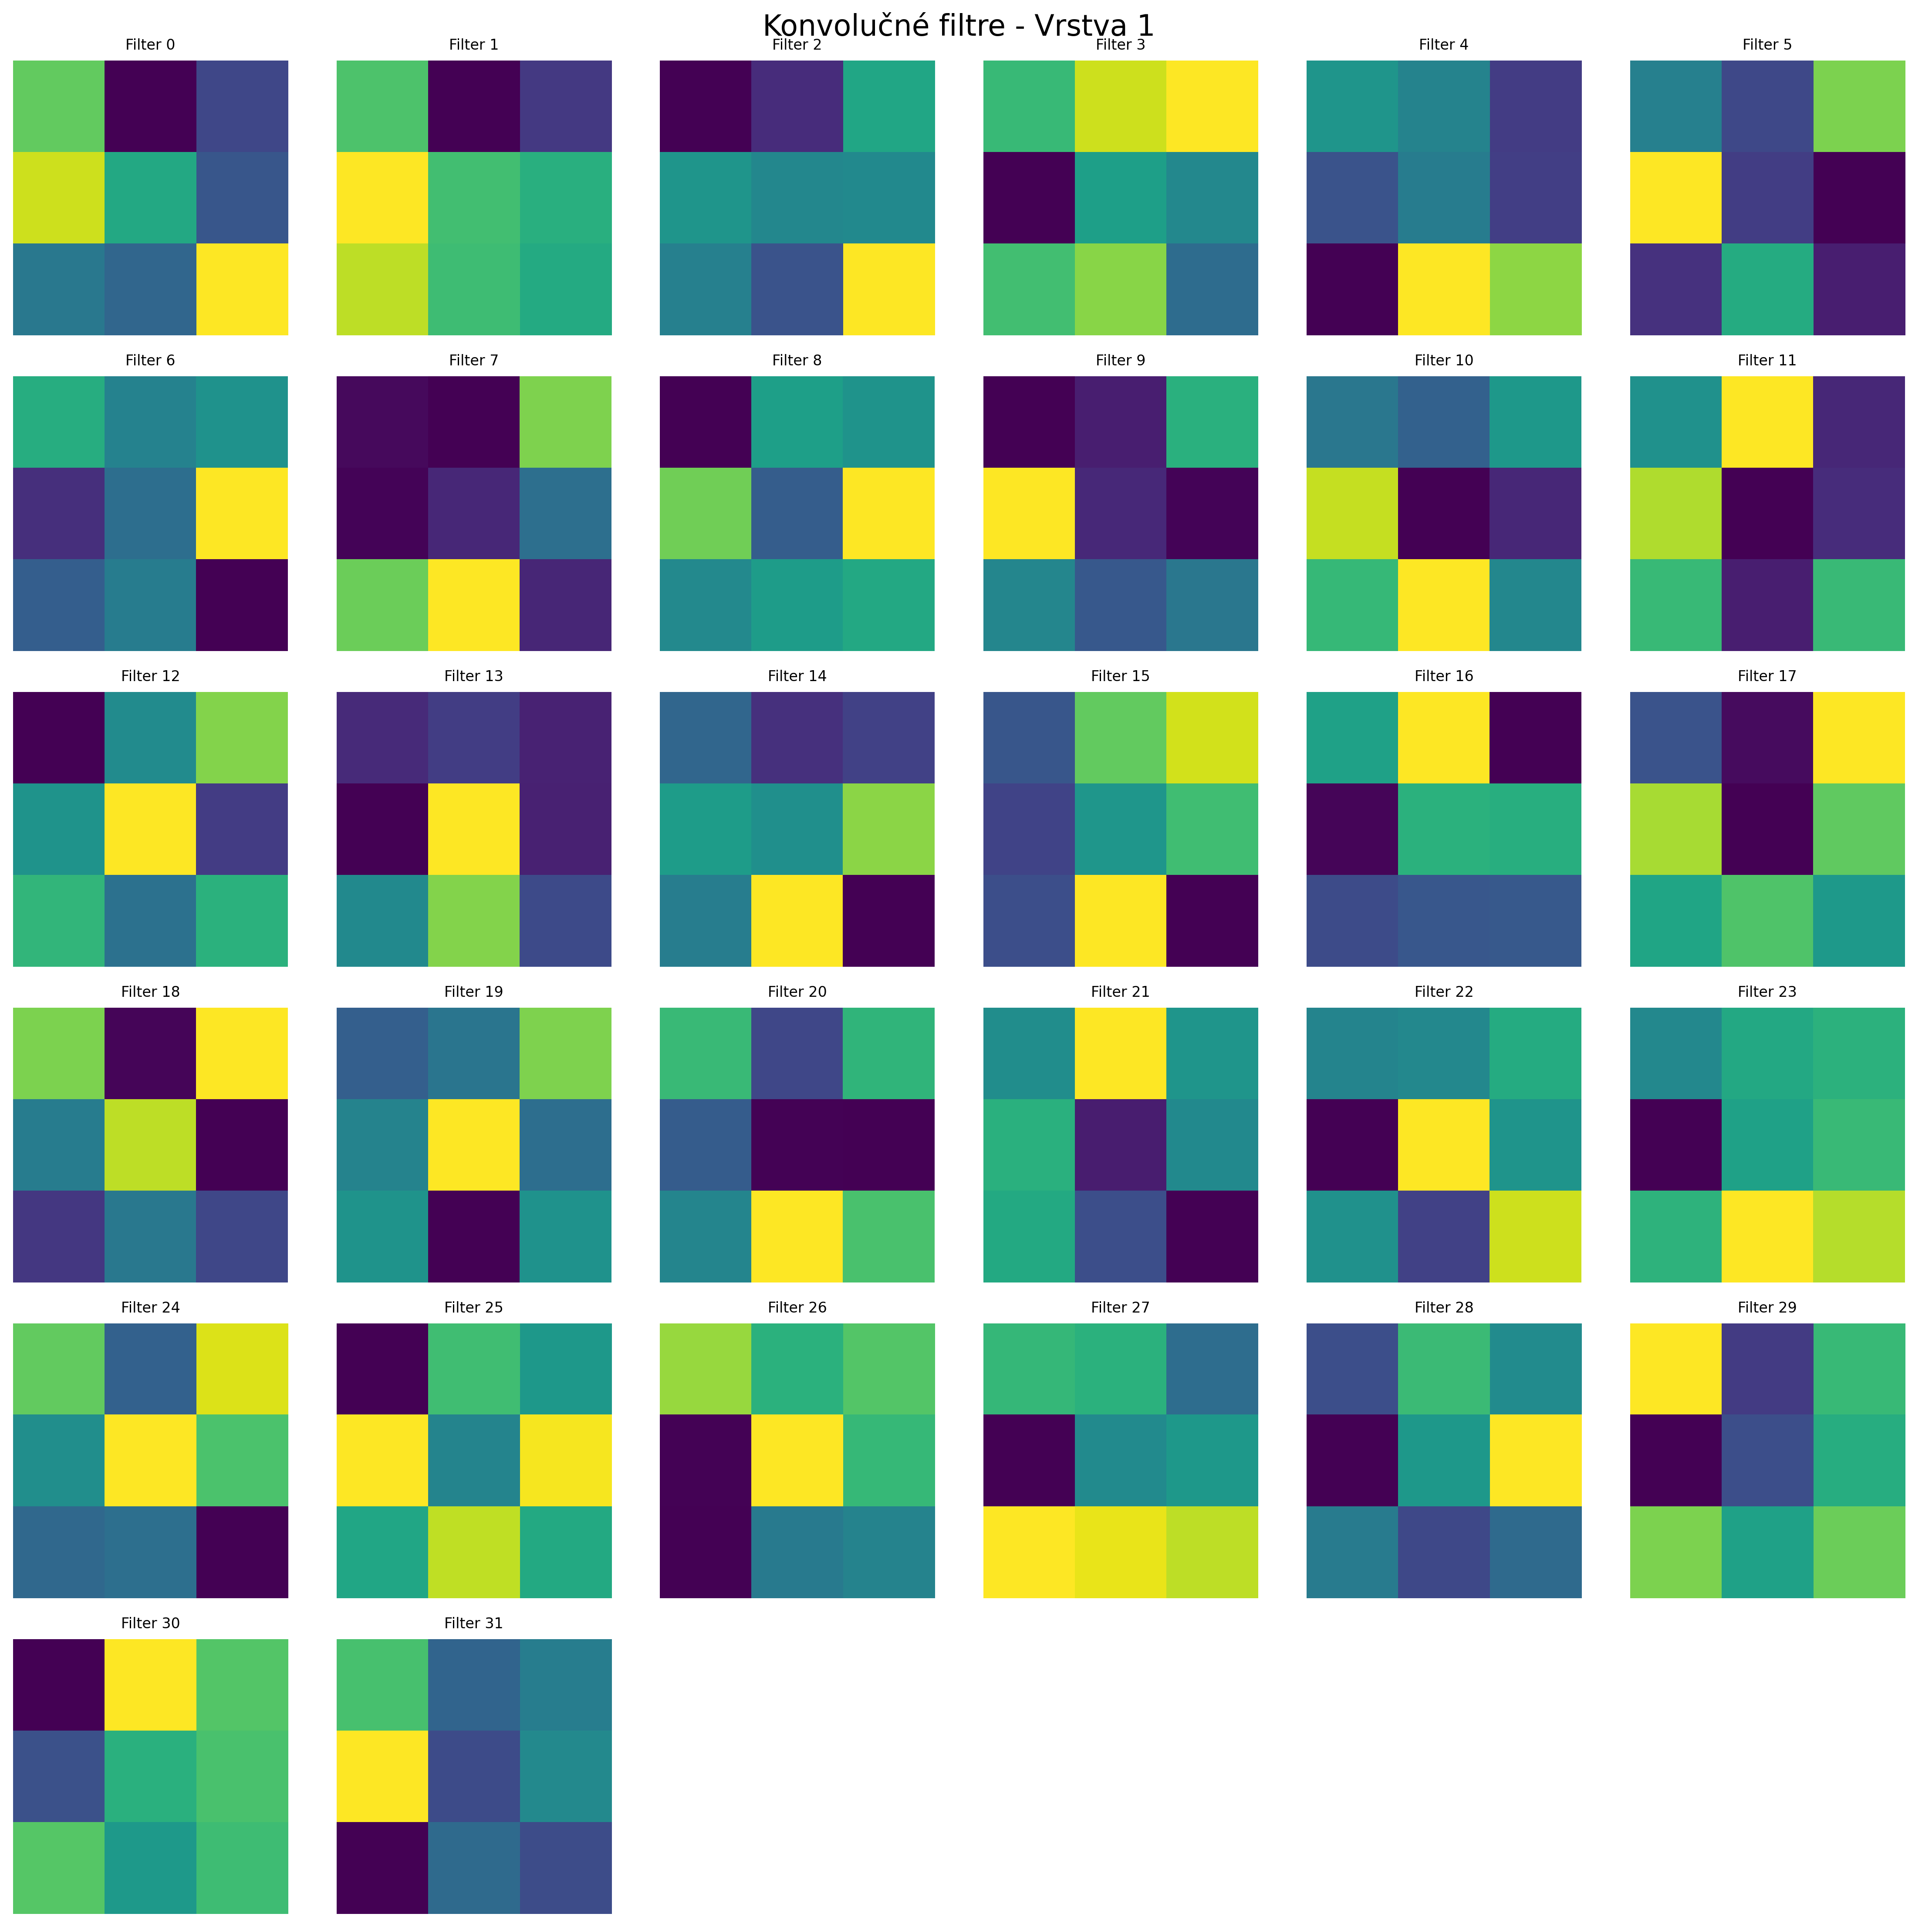
\includegraphics[width=1.1\textwidth]{../figures/conv_filters_layer_1_config_5.png}
    \caption{Filtre druhej konvolučnej vrstvy}
    \label{fig:conv_filters_layer_1}
\end{figure}

\clearpage

\subsection{Bonus: Testovanie na vlastných obrázkoch}

Model bol testovaný na 5 vlastných fotografiách oblohy z~Bratislavy:

\begin{figure}[H]
    \centering
    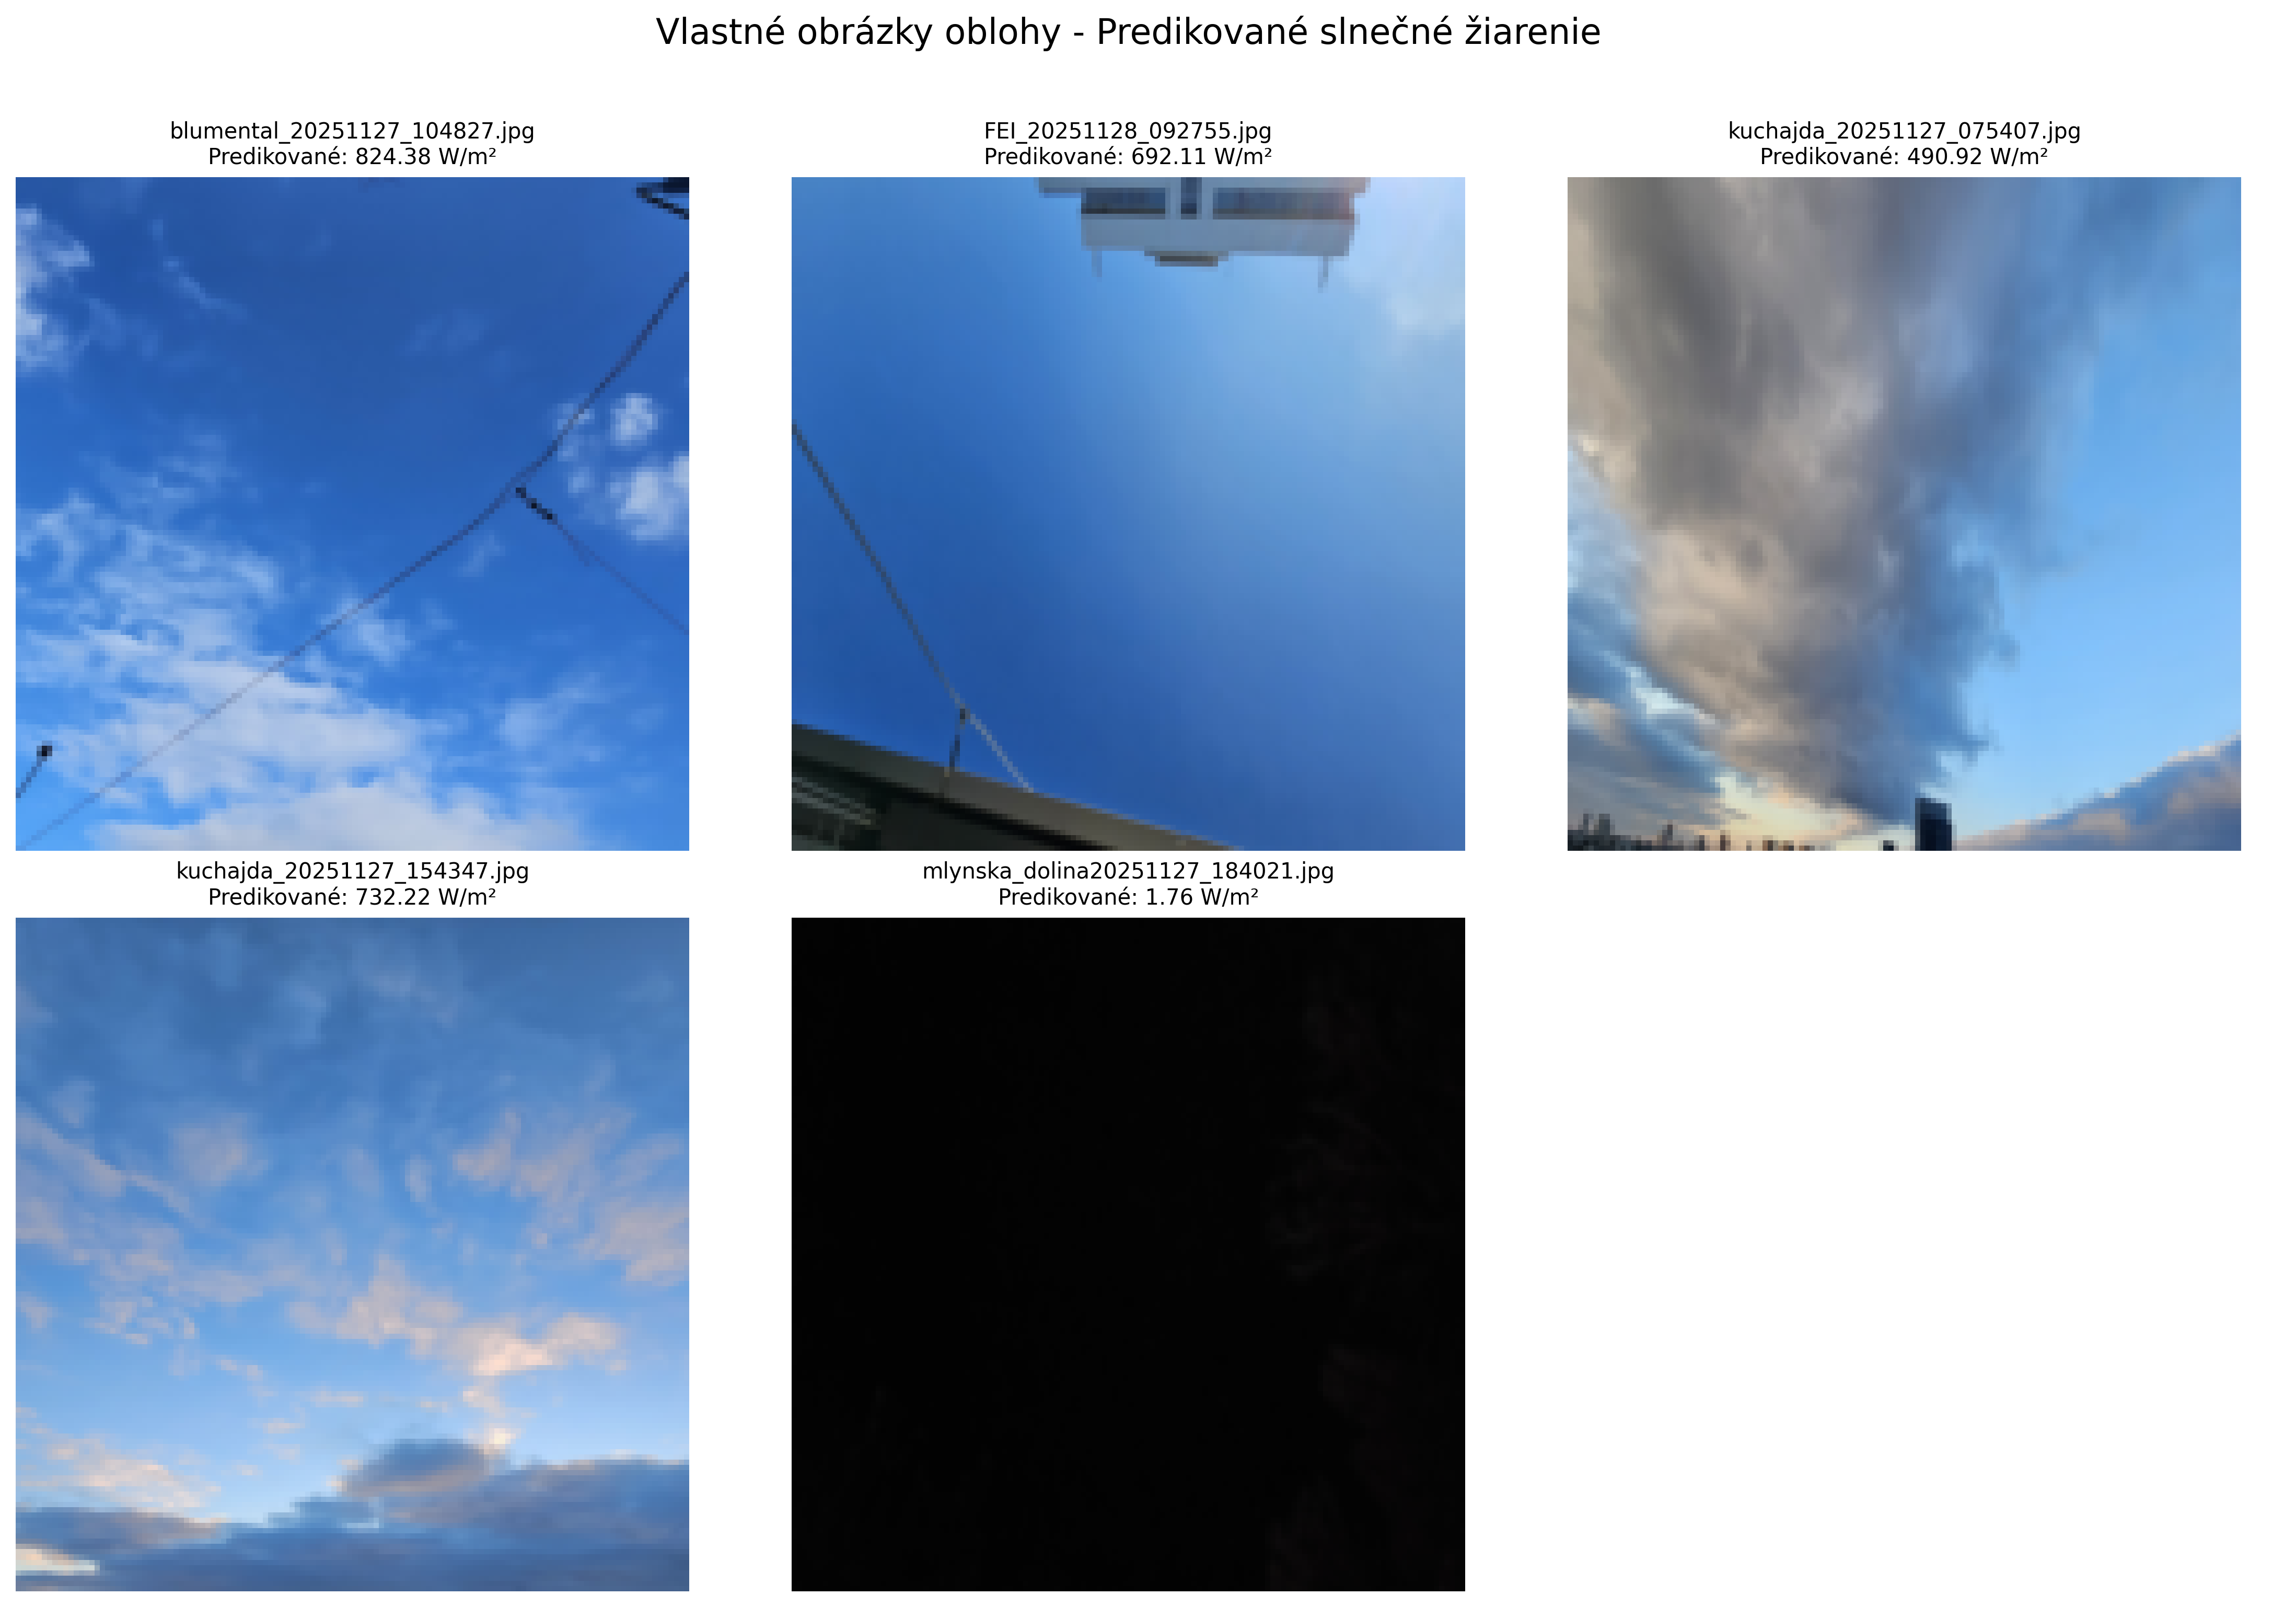
\includegraphics[width=1.1\textwidth]{../figures/custom_images_predictions_config_5.png}
    \caption{Predikcie na vlastných obrázkoch oblohy}
    \label{fig:custom_predictions}
\end{figure}

\begin{table}[H]
\centering
\begin{tabular}{lr}
\toprule
\textbf{Obrázok} & \textbf{Predikcia (W/m²)} \\
\midrule
blumental\_20251127\_104827.jpg & 824.38 \\
FEI\_20251128\_092755.jpg & 692.11 \\
kuchajda\_20251127\_075407.jpg & 490.92 \\
kuchajda\_20251127\_154347.jpg & 732.22 \\
mlynska\_dolina20251127\_184021.jpg & 1.76 \\
\bottomrule
\end{tabular}
\caption{Predikcie na vlastných obrázkoch}
\end{table}

\textbf{Interpretácia:}
\begin{itemize}
    \item Model správne rozpoznal vysoké žiarenie pri jasnej oblohe
    \item Večerný/nočný obrázok správne klasifikovaný s~nízkym žiarením (1.76 W/m²)
\end{itemize}

\clearpage

\subsection{Bonus: Predikcia žiarenia o~15 minút}

Vytvorili sme model na predikciu budúceho žiarenia z~aktuálneho obrázka:

\begin{table}[H]
\centering
\begin{tabular}{lrr}
\toprule
\textbf{Úloha} & \textbf{R²} & \textbf{RMSE} \\
\midrule
Odhad aktuálneho žiarenia & 0.9744 & 45.43 \\
Predikcia o~15 minút & 0.5901 & 180.40 \\
\bottomrule
\end{tabular}
\caption{Porovnanie odhadu vs. predikcie}
\end{table}

\begin{figure}[H]
    \centering
    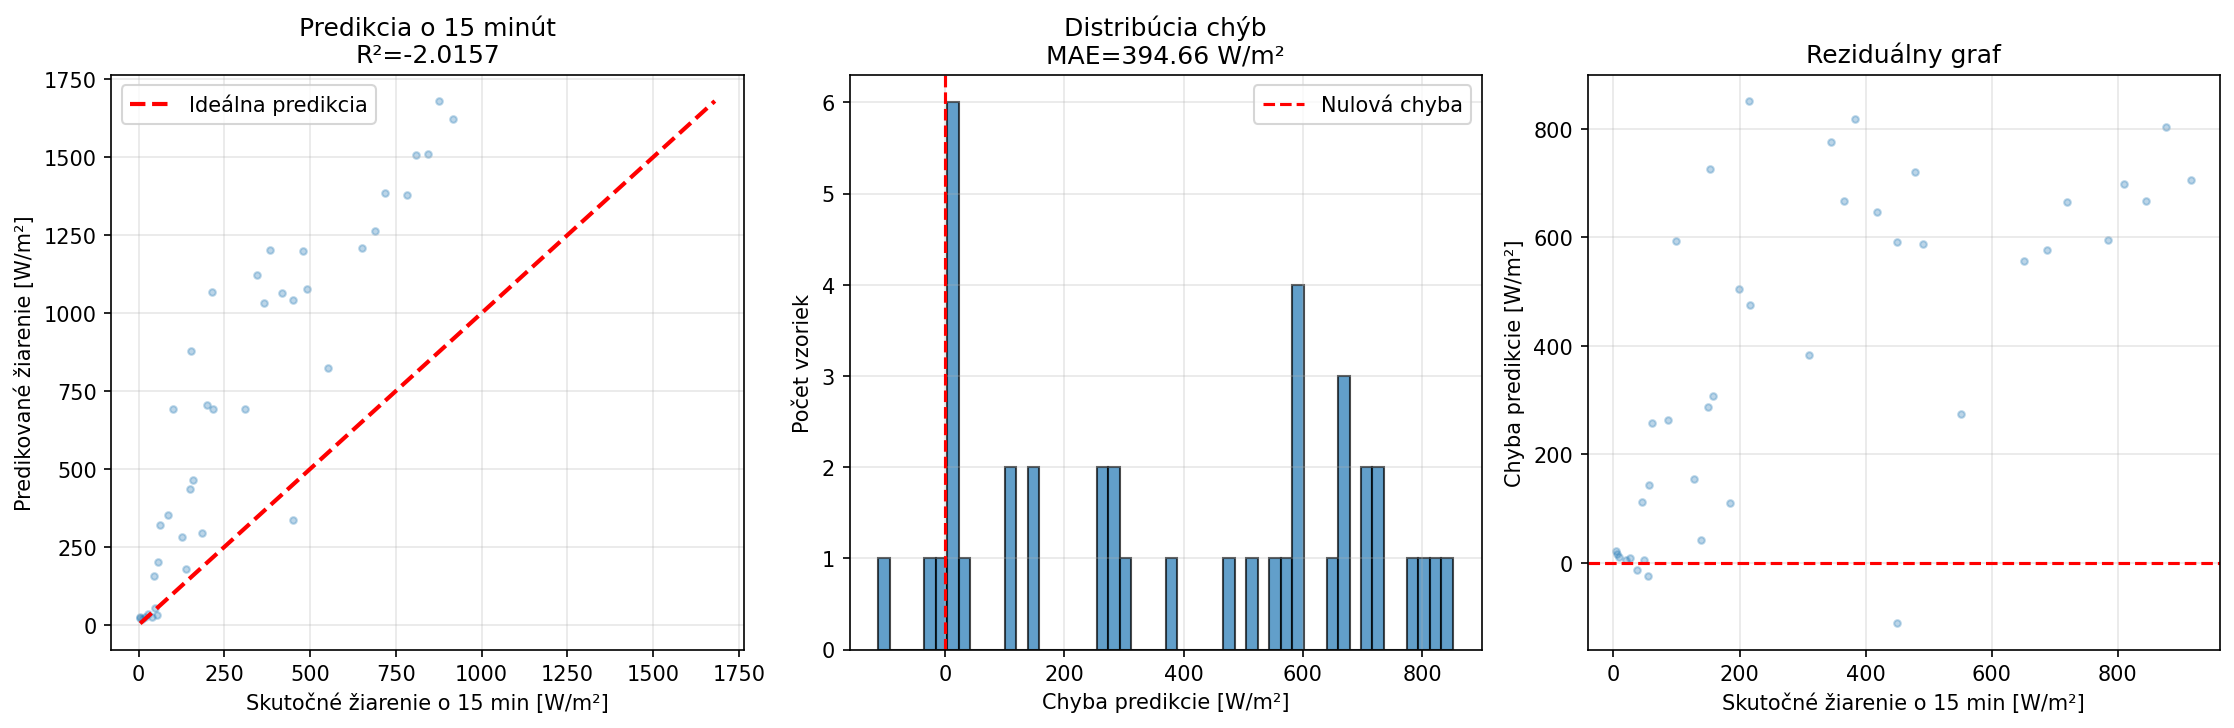
\includegraphics[width=1.1\textwidth]{../figures/bonus_prediction_15min.png}
    \caption{Výsledky predikcie žiarenia o~15 minút}
    \label{fig:prediction_15min}
\end{figure}

\textbf{Zistenie:} Predikcia budúceho žiarenia je výrazne ťažšia úloha kvôli dynamickým zmenám oblačnosti.

\clearpage

\section{Transfer Learning a~zhlukovanie}

\subsection{Extrakcia príznakov pomocou MobileNetV2}

Pre transfer learning sme použili predtrénovaný model \textbf{MobileNetV2}:

\begin{itemize}
    \item Predtrénovaný na ImageNet datasete
    \item Extrahované príznaky z~poslednej konvolučnej vrstvy
    \item Veľkosť výstupného feature vektora: \textbf{62~720} dimenzií
\end{itemize}

\subsubsection{Redukcia dimenzie pomocou PCA}

\begin{table}[H]
\centering
\begin{tabular}{lr}
\toprule
\textbf{Parameter} & \textbf{Hodnota} \\
\midrule
Pôvodná dimenzia & 62~720 \\
Redukovaná dimenzia (zhlukovanie) & 50 \\
Redukovaná dimenzia (regresia) & 300 \\
Vysvetlený rozptyl (50 komponentov) & 74.81\% \\
Vysvetlený rozptyl (300 komponentov) & 90.07\% \\
\bottomrule
\end{tabular}
\caption{Parametre PCA redukcie}
\end{table}

\subsection{Zhlukovanie pomocou K-Means}

\subsubsection{Výber optimálneho počtu zhlukov}

Použili sme Elbow Method a~Silhouette Analysis:

\begin{itemize}
    \item Testované k = 2 až 10
    \item \textbf{Vybraný počet zhlukov: 7}
\end{itemize}

\clearpage

\subsubsection{Vizualizácia zhlukov (t-SNE)}

\begin{figure}[H]
    \centering
    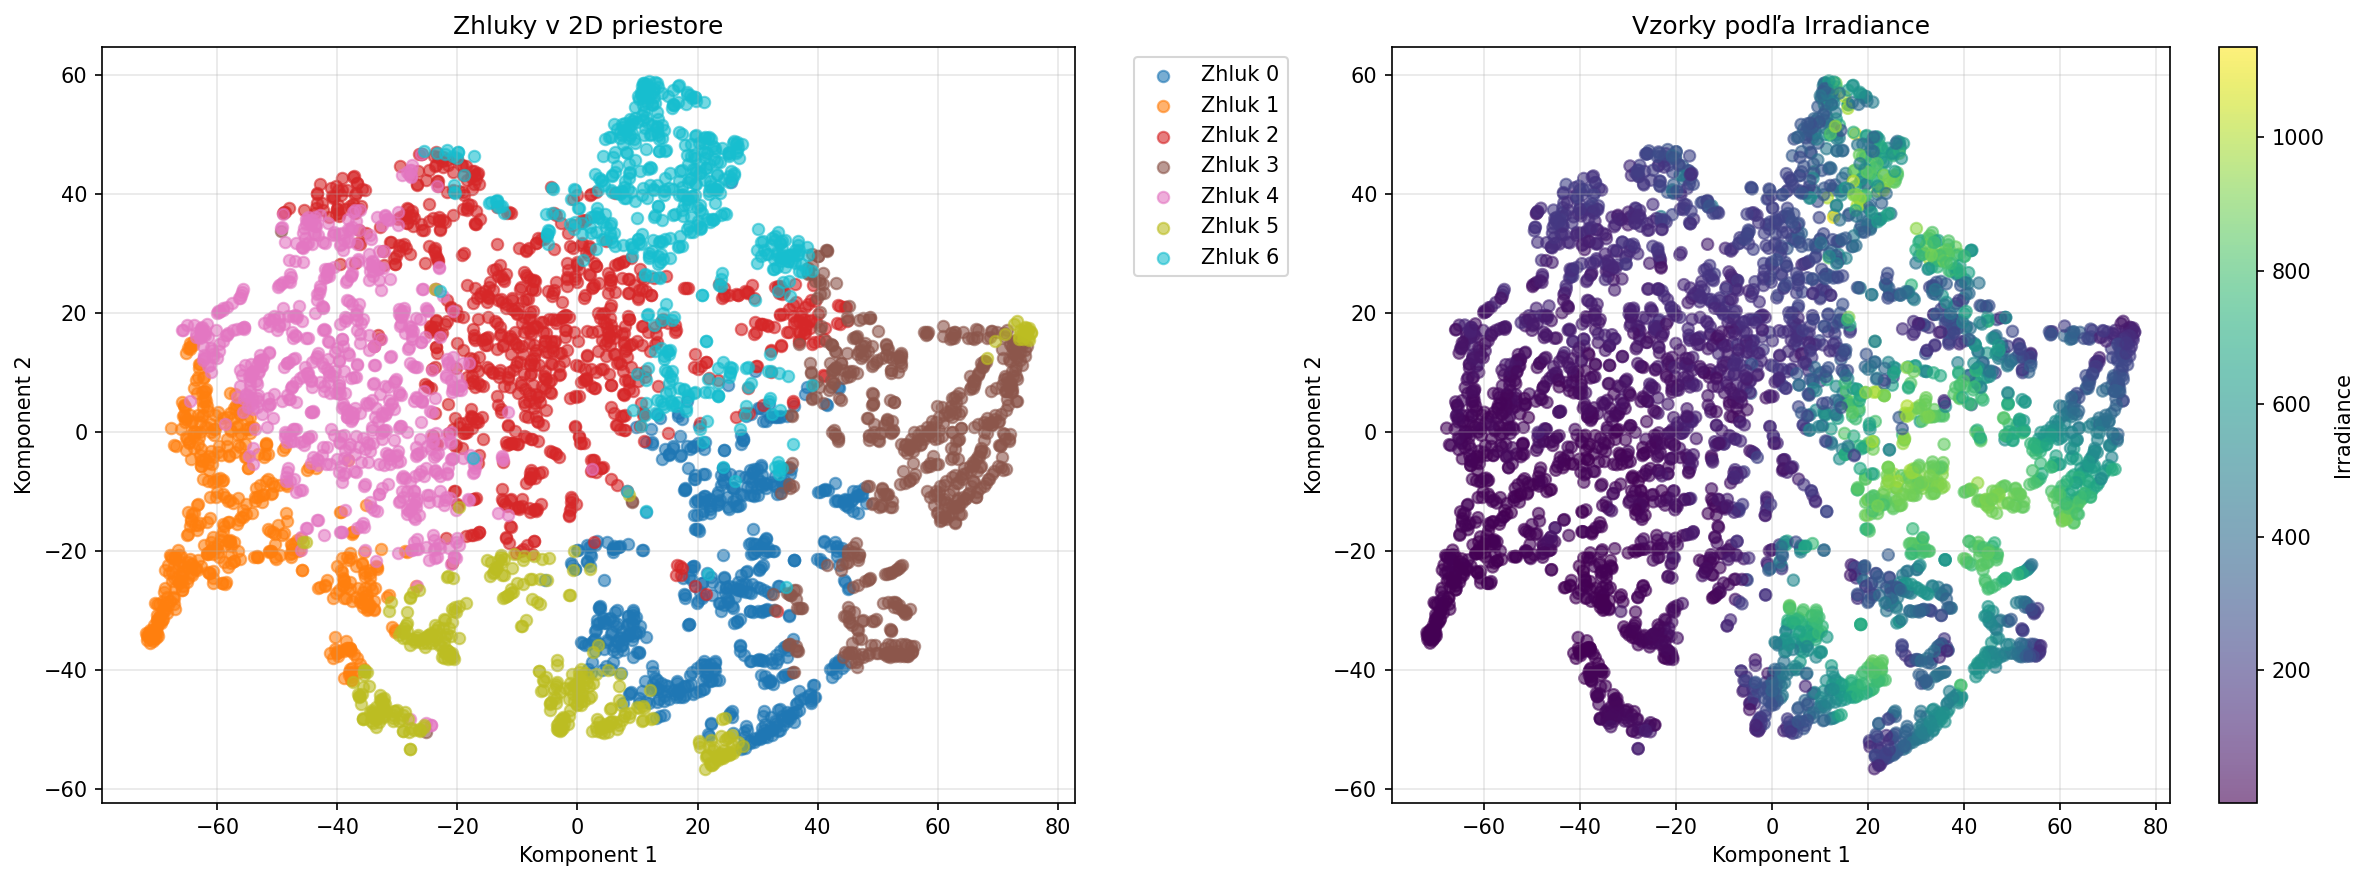
\includegraphics[width=1.1\textwidth]{../figures/clusters_2d.png}
    \caption{2D vizualizácia zhlukov pomocou t-SNE}
    \label{fig:clusters_2d}
\end{figure}

\subsubsection{Priemerné obrázky pre každý zhluk}

\begin{figure}[H]
    \centering
    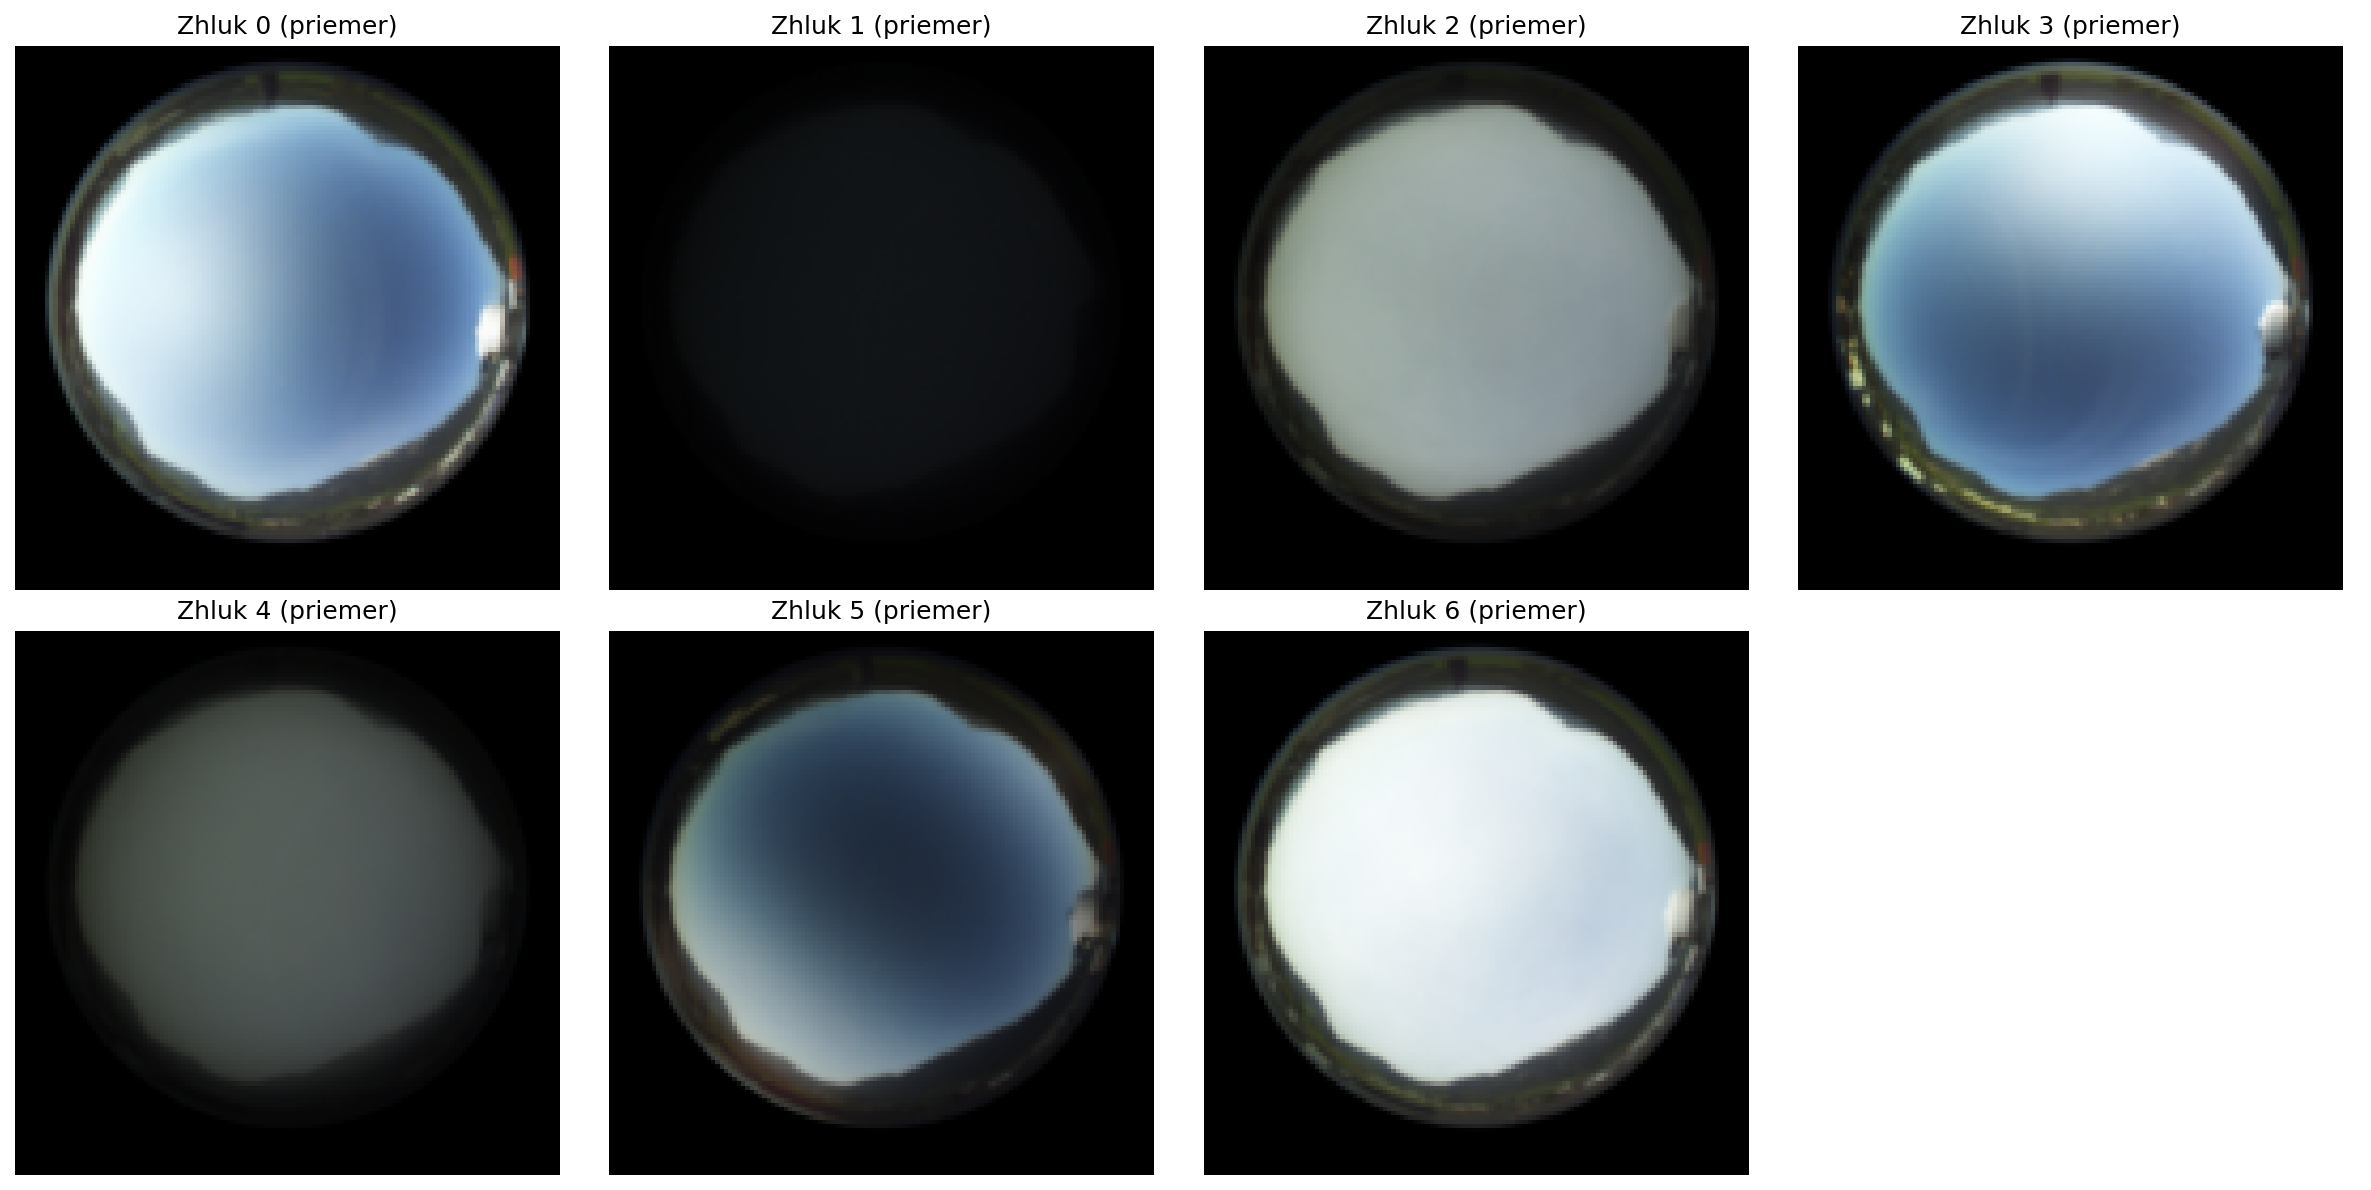
\includegraphics[width=1.1\textwidth]{../figures/average_cluster_images.png}
    \caption{Priemerné obrázky pre jednotlivé zhluky}
    \label{fig:average_cluster_images}
\end{figure}

\clearpage

\subsubsection{Distribúcia Irradiance podľa zhlukov}

\begin{figure}[H]
    \centering
    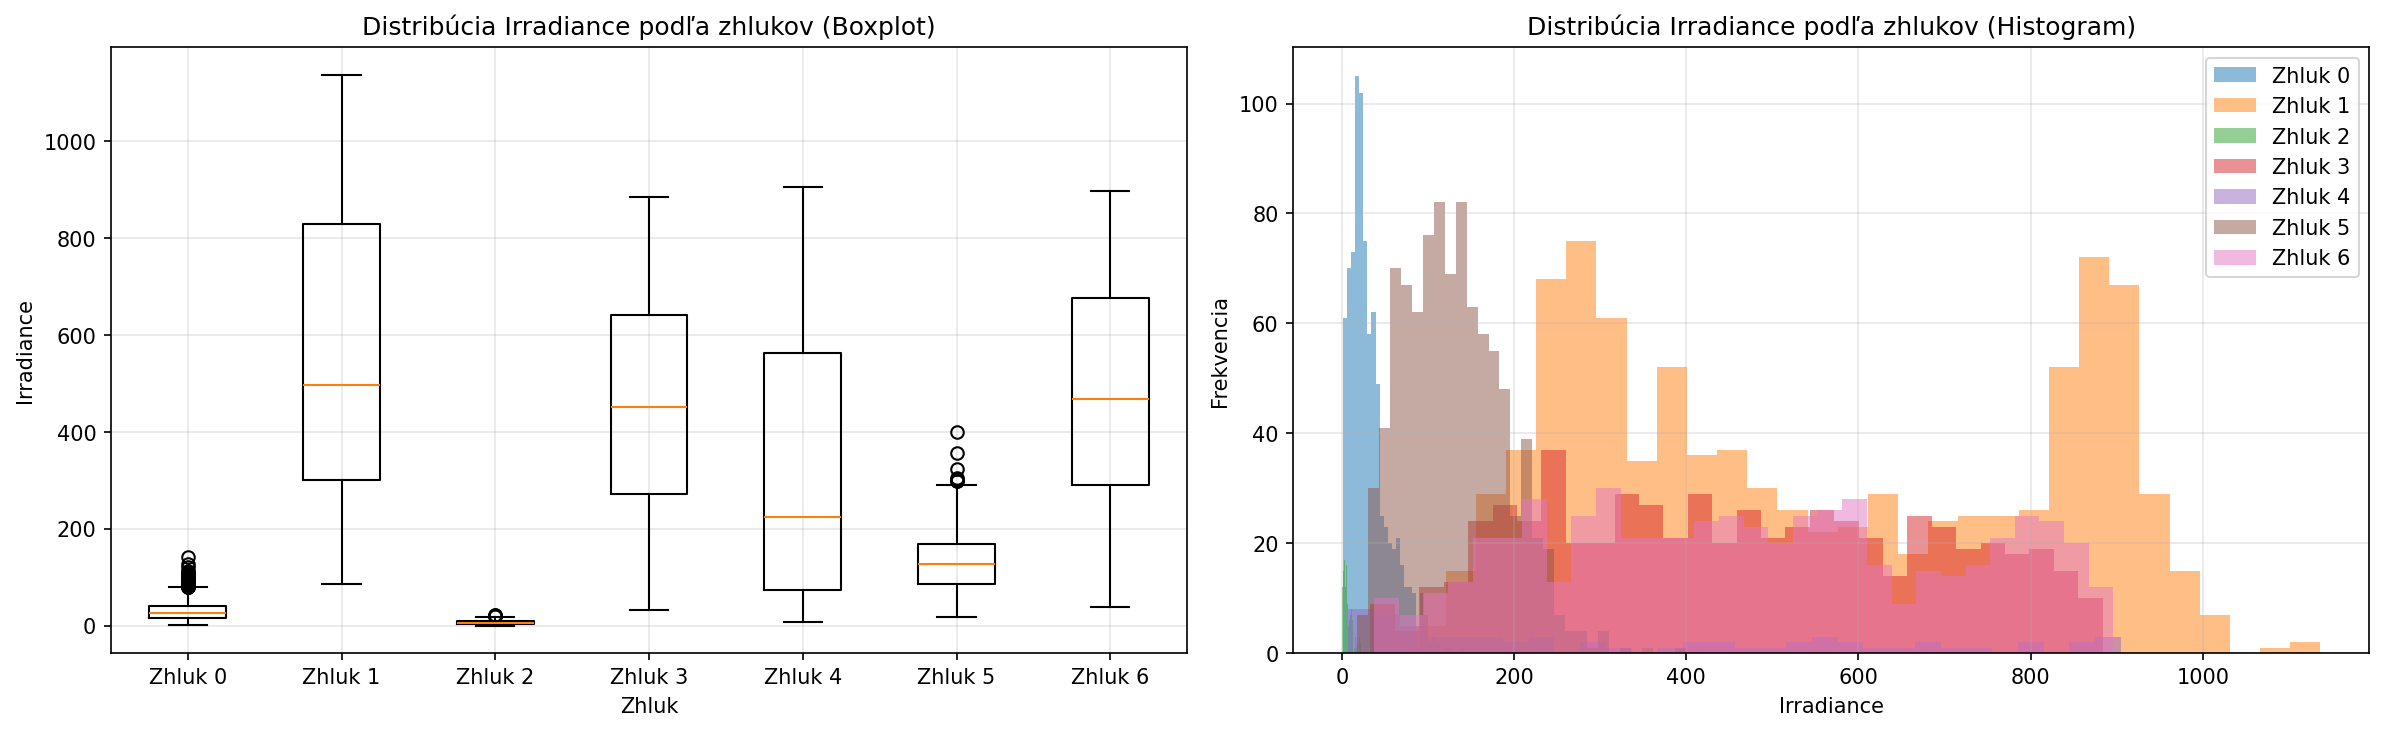
\includegraphics[width=1.1\textwidth]{../figures/cluster_irradiance_distribution.png}
    \caption{Distribúcia slnečného žiarenia v~jednotlivých zhlukoch}
    \label{fig:cluster_distribution}
\end{figure}

\textbf{Interpretácia zhlukov:}
\begin{itemize}
    \item Zhluky s~nízkym priemerným žiarením (< 100 W/m²): nočné/zamračené obdobia
    \item Zhluky so stredným žiarením (100--600 W/m²): polojasno, čiastočne oblačno
    \item Zhluky s~vysokým žiarením (> 600 W/m²): jasná obloha, priame slnko
\end{itemize}

\clearpage

\subsection{Transfer Learning - Stacking Ensemble}

Pre regresiu sme použili Stacking Ensemble kombinujúci:
\begin{itemize}
    \item \textbf{Gradient Boosting Regressor} (500 estimátorov, max\_depth=8)
    \item \textbf{Random Forest Regressor} (300 estimátorov, max\_depth=15)
    \item \textbf{Ridge Regression} ako finálny estimátor
\end{itemize}

\subsubsection{Vstupy modelu}

\begin{itemize}
    \item 300 PCA komponentov z~MobileNetV2 príznakov
    \item 2 tabuľkové príznaky (Pressure, Humidity)
    \item \textbf{Celkovo: 302 príznakov}
\end{itemize}

\subsubsection{Výsledky Transfer Learning}

\begin{table}[H]
\centering
\begin{tabular}{lrrrr}
\toprule
\textbf{Množina} & \textbf{R²} & \textbf{RMSE} & \textbf{MAE} & \textbf{MSE} \\
\midrule
Trénovacia & 0.9976 & -- & -- & -- \\
Validačná & 0.9586 & -- & -- & -- \\
Testovacia & 0.9601 & 56.73 & 29.15 & 3218.05 \\
\bottomrule
\end{tabular}
\caption{Výsledky Transfer Learning modelu}
\end{table}

\clearpage

\subsection{Porovnanie CNN vs. Transfer Learning}

\begin{table}[H]
\centering
\begin{tabular}{lrrr}
\toprule
\textbf{Model} & \textbf{Test R²} & \textbf{Test RMSE} & \textbf{Test MAE} \\
\midrule
CNN (Konfigurácia 5) & 0.9744 & 45.43 & 31.37 \\
Transfer Learning (Stacking) & 0.9601 & 56.73 & 29.15 \\
\midrule
\textbf{Rozdiel} & -0.0143 & +11.30 & -2.22 \\
\bottomrule
\end{tabular}
\caption{Porovnanie CNN a~Transfer Learning}
\end{table}

\textbf{Analýza:}
\begin{itemize}
    \item CNN dosahuje vyššie R² a~nižšie RMSE
    \item Transfer Learning má nižšie MAE -- menšie priemerné chyby
    \item Oba prístupy dosahujú vysokú presnosť (R² > 0.96)
\end{itemize}

\subsection{Vizualizácia výsledkov Transfer Learning}

\begin{figure}[H]
    \centering
    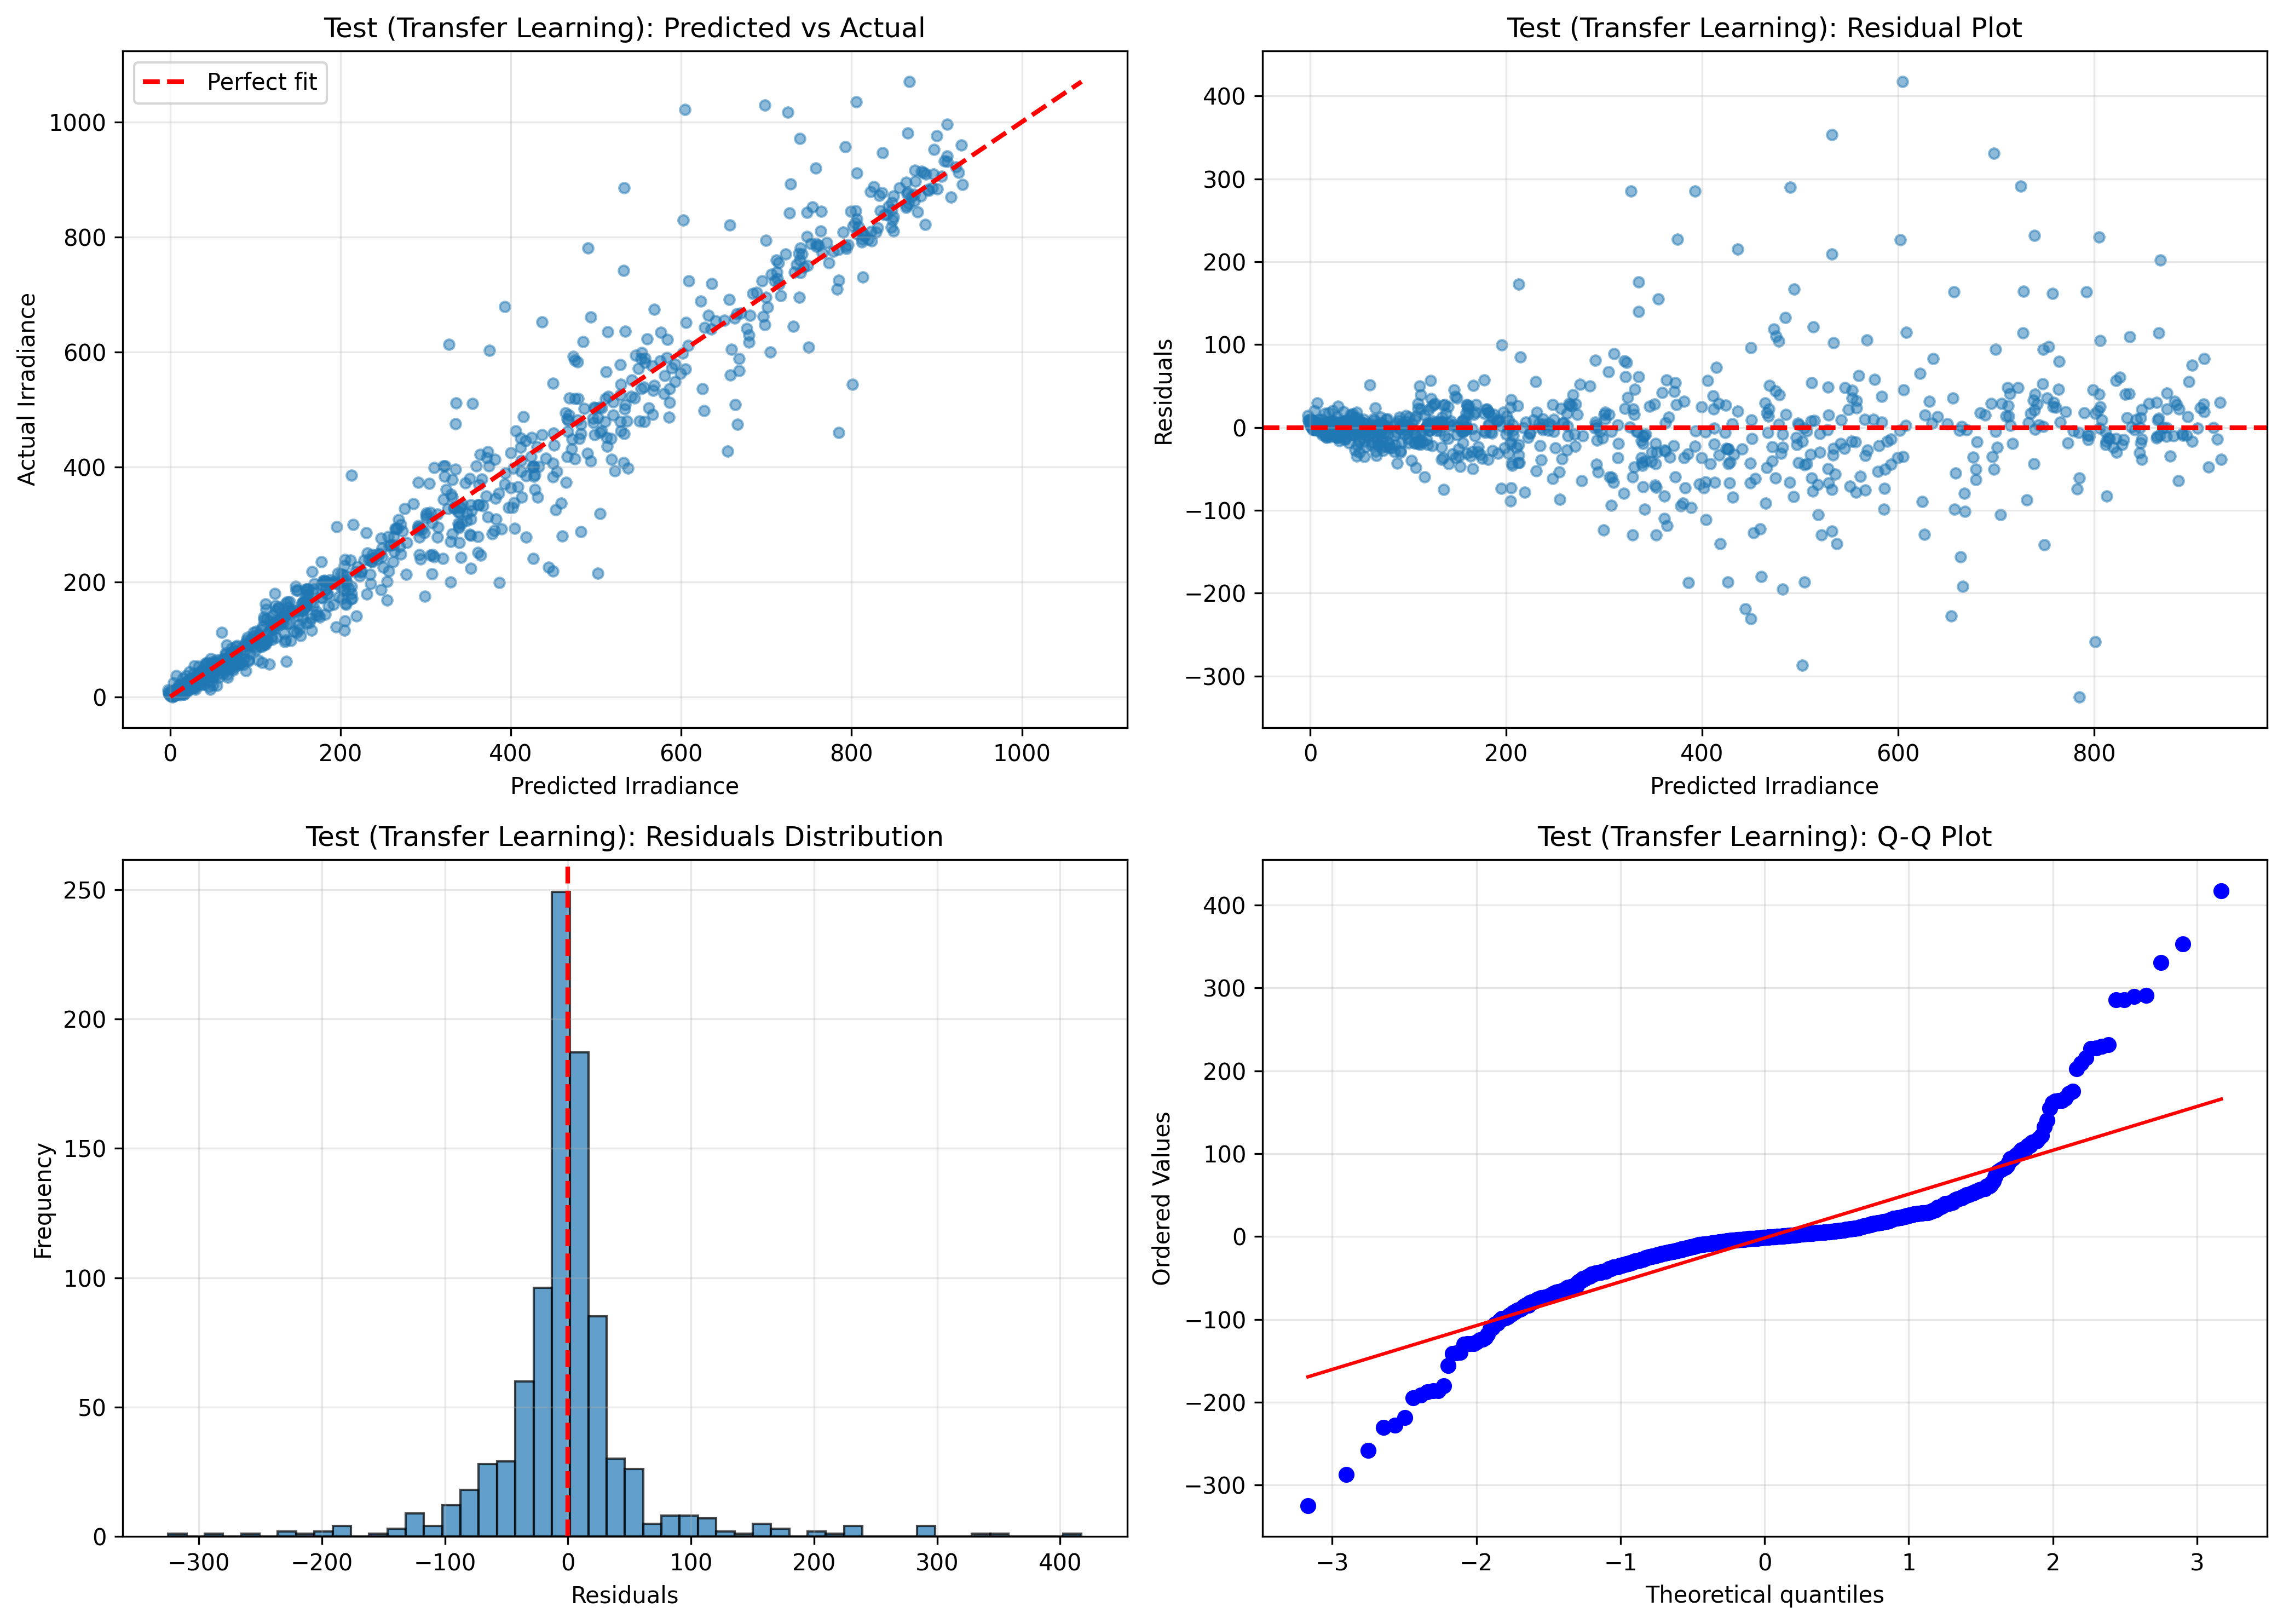
\includegraphics[width=1.1\textwidth]{../figures/transfer_learning_residuals.png}
    \caption{Reziduálna analýza Transfer Learning modelu}
    \label{fig:tl_residuals}
\end{figure}

\clearpage

\begin{figure}[H]
    \centering
    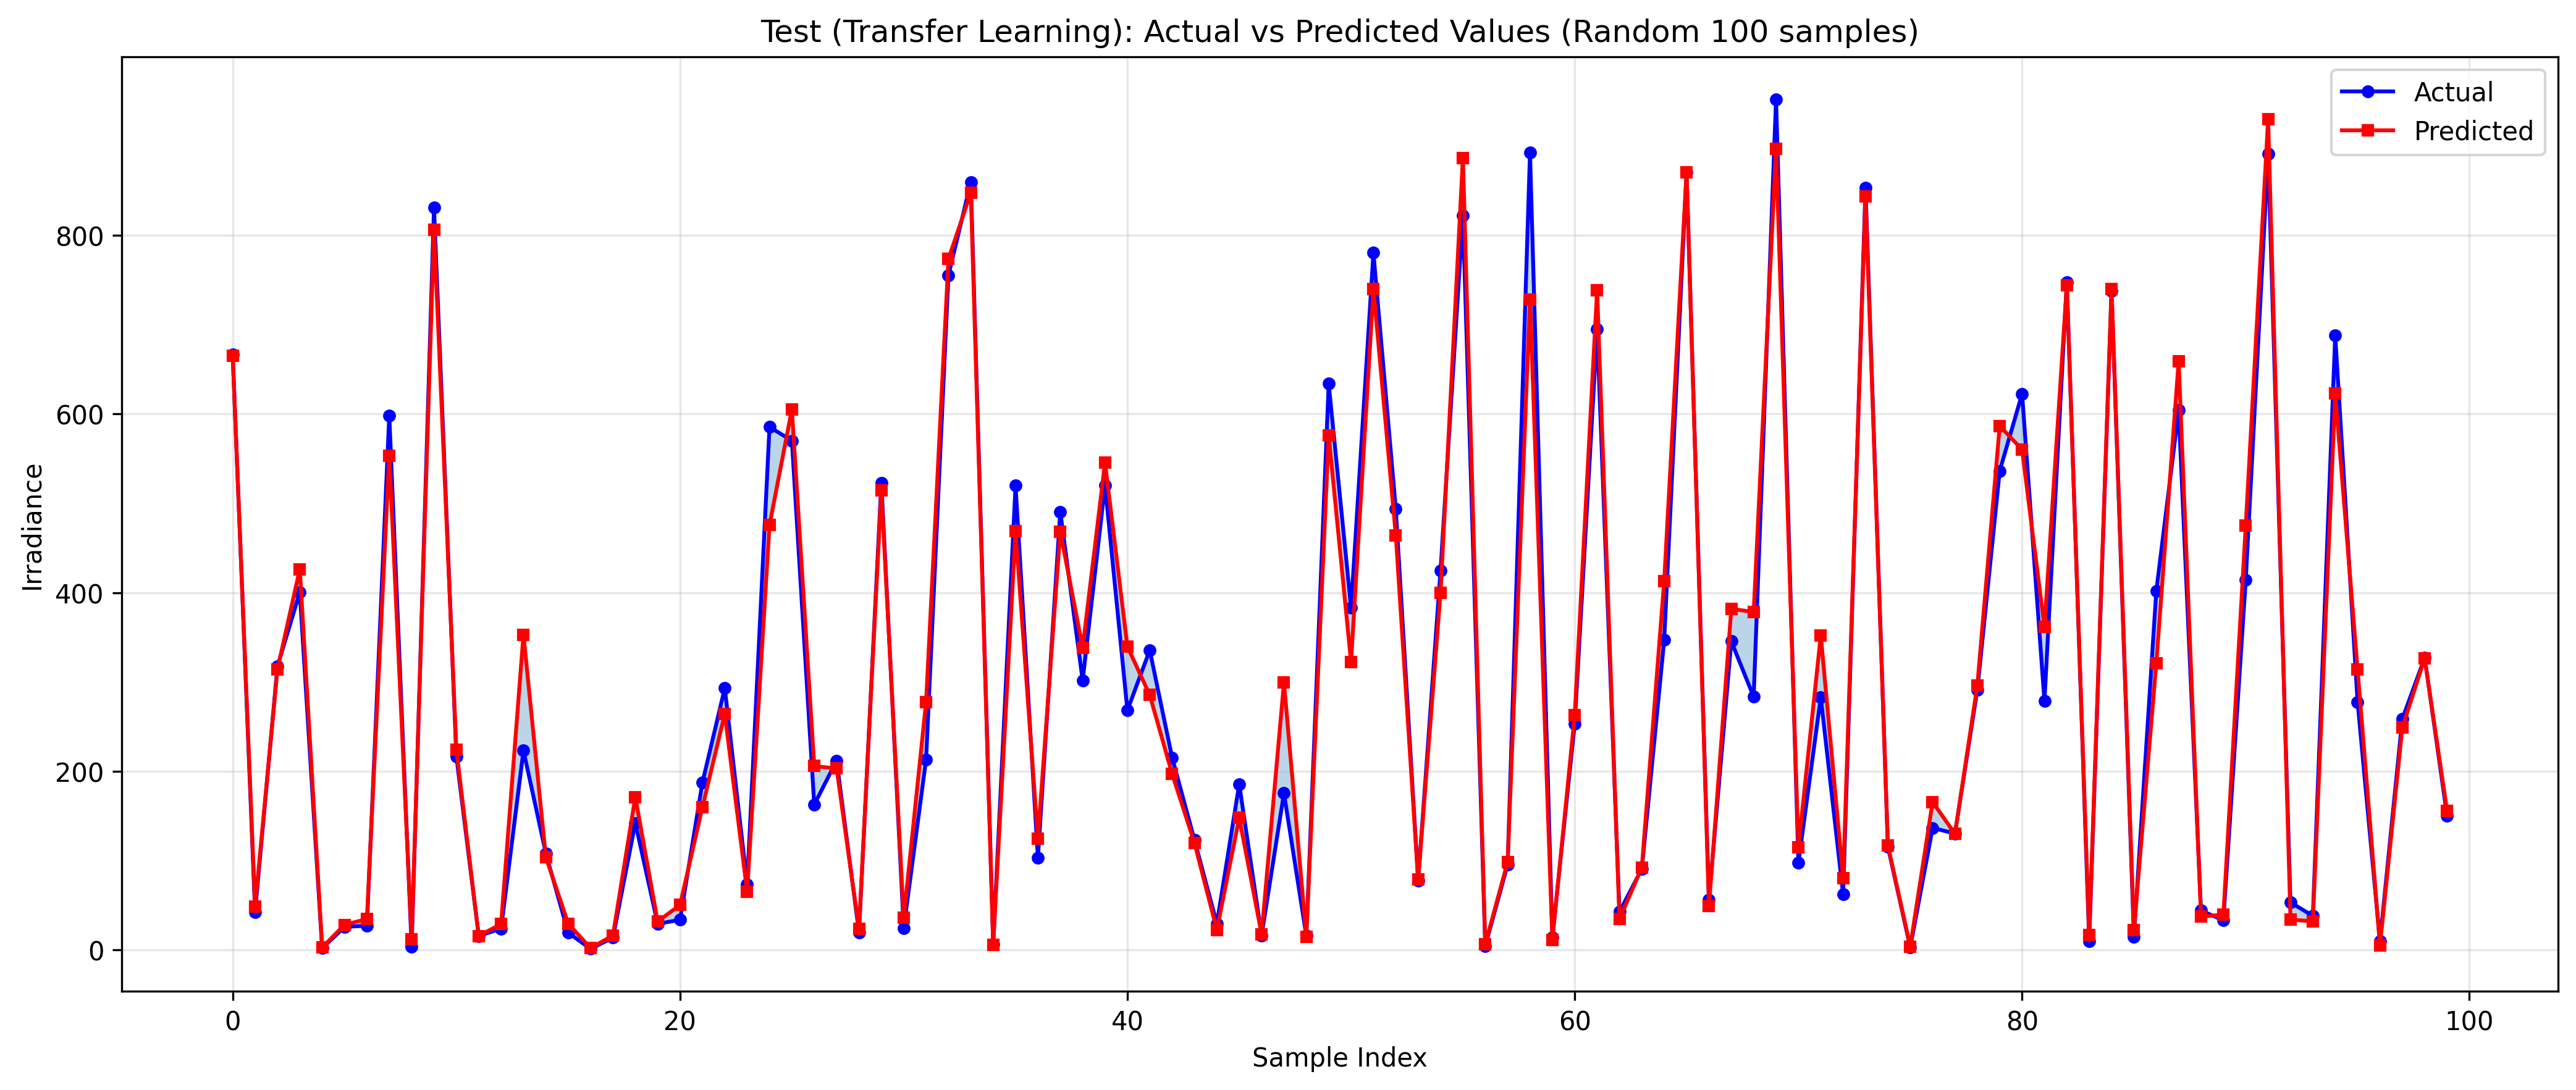
\includegraphics[width=1.1\textwidth]{../figures/transfer_learning_predictions.png}
    \caption{Porovnanie predikcií Transfer Learning modelu}
    \label{fig:tl_predictions}
\end{figure}

\subsection{Analýza najhorších predikcií}

\begin{figure}[H]
    \centering
    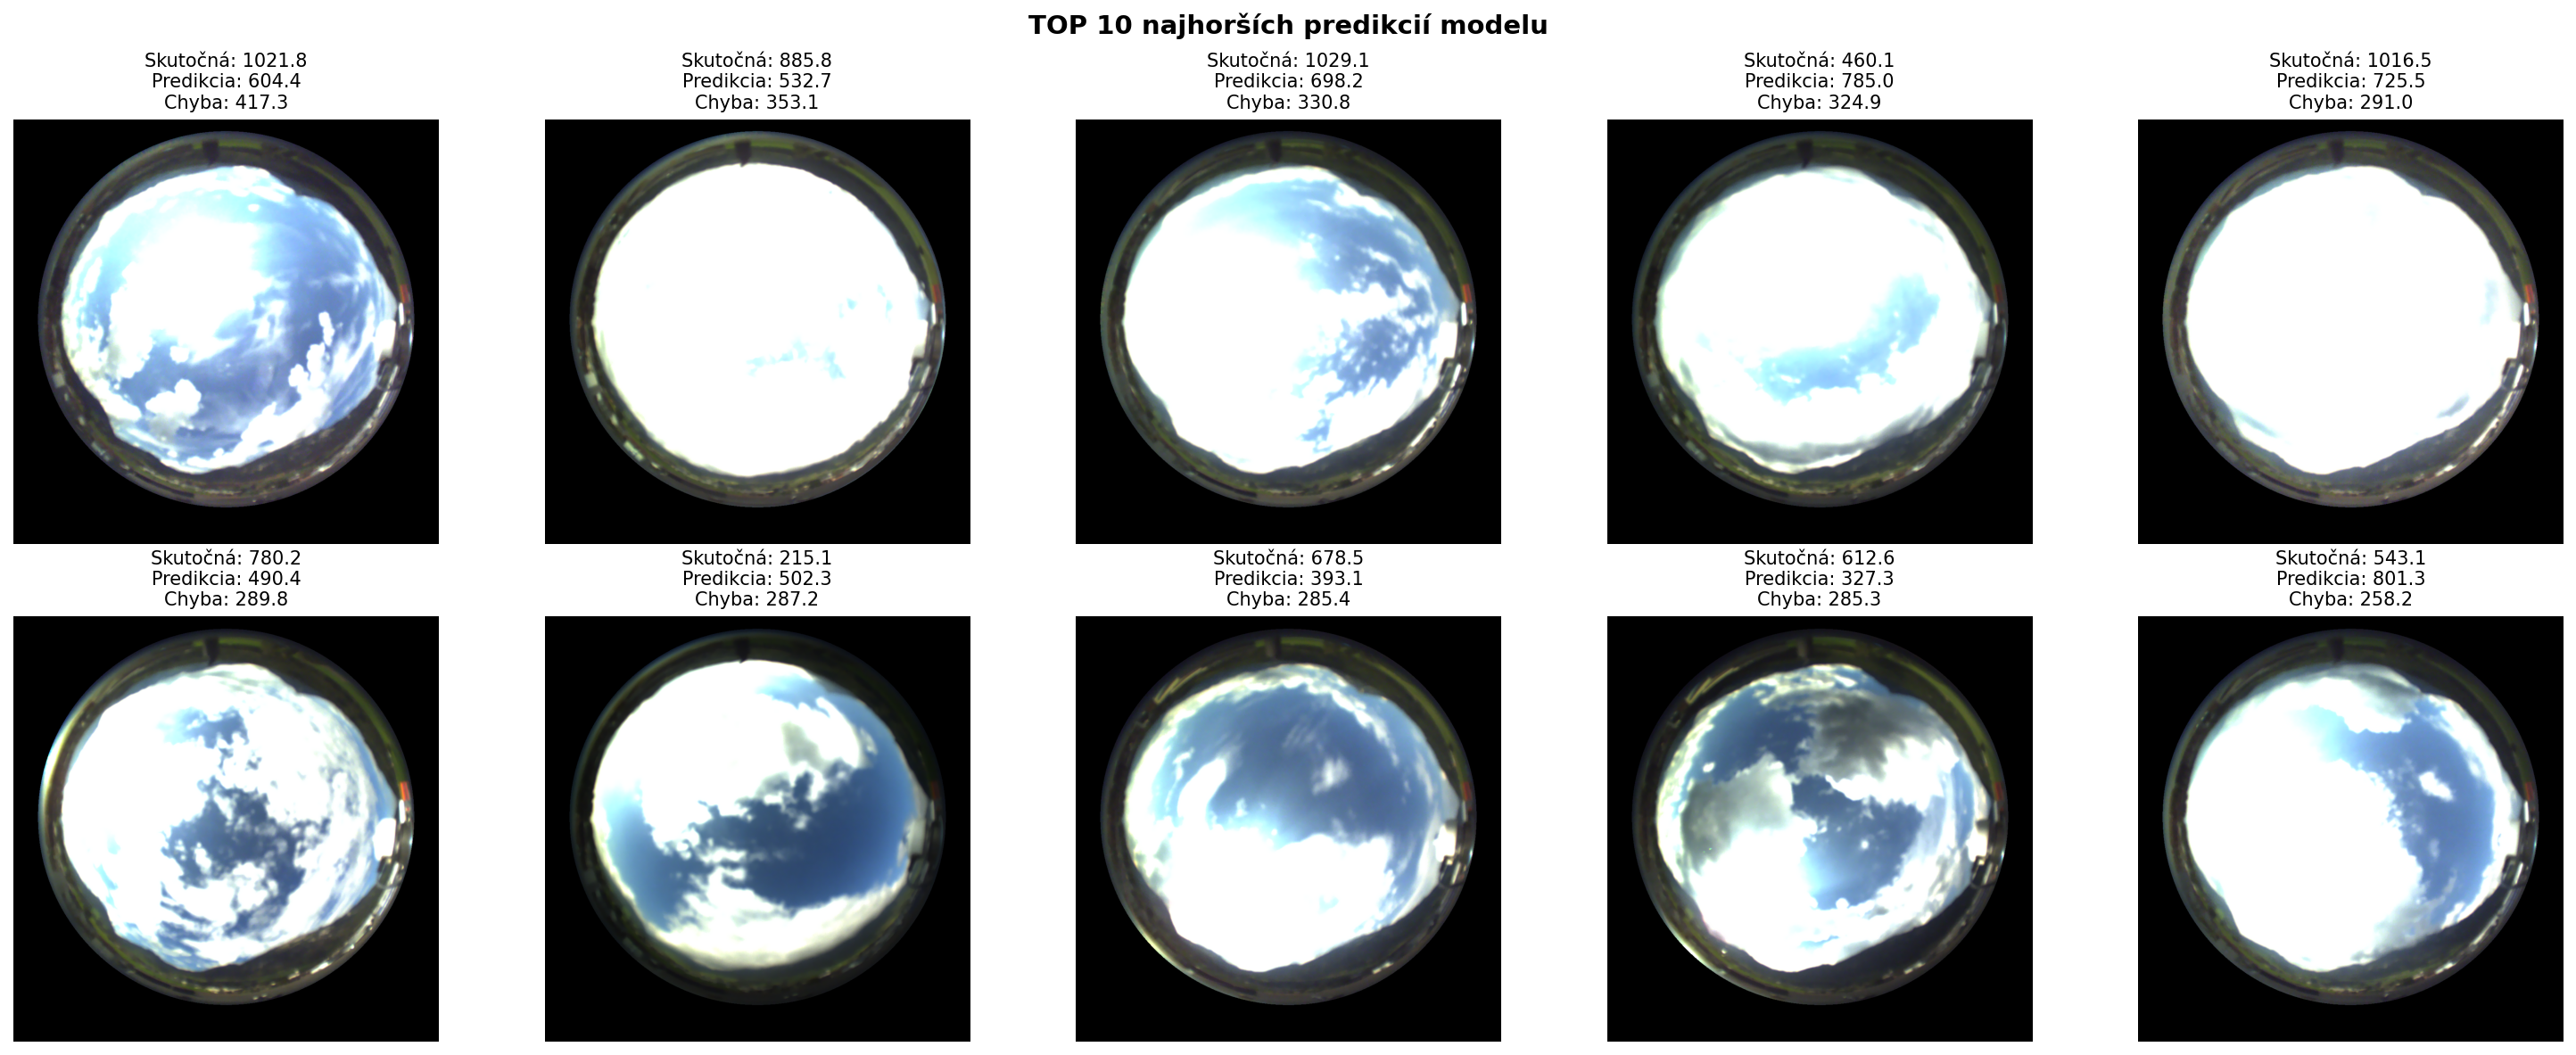
\includegraphics[width=1.1\textwidth]{../figures/worst_predictions.png}
    \caption{Top 10 najhorších predikcií modelu}
    \label{fig:worst_predictions}
\end{figure}

\textbf{Model má tendenciu robiť najväčšie chyby pri:}
\begin{itemize}
    \item Extrémnych hodnotách žiarenia
    \item Prechodových podmienkach (čiastočne oblačno)
    \item Neobvyklých poveternostných situáciách
\end{itemize}

\clearpage

\subsection{Bonus: Fúzia modelov}

Porovnali sme výkon modelov s~rôznymi typmi príznakov:

\begin{table}[H]
\centering
\begin{tabular}{lrrr}
\toprule
\textbf{Model} & \textbf{R²} & \textbf{RMSE} & \textbf{MAE} \\
\midrule
Obrazové príznaky (PCA 50) & 0.9561 & 59.52 & 32.88 \\
Tabuľkové príznaky & 0.7722 & 135.59 & 92.08 \\
\textbf{Fúzia (obrazové + tabuľkové)} & \textbf{0.9574} & \textbf{58.64} & \textbf{32.29} \\
\bottomrule
\end{tabular}
\caption{Porovnanie modelov s~rôznymi príznakmi}
\end{table}

\begin{figure}[H]
    \centering
    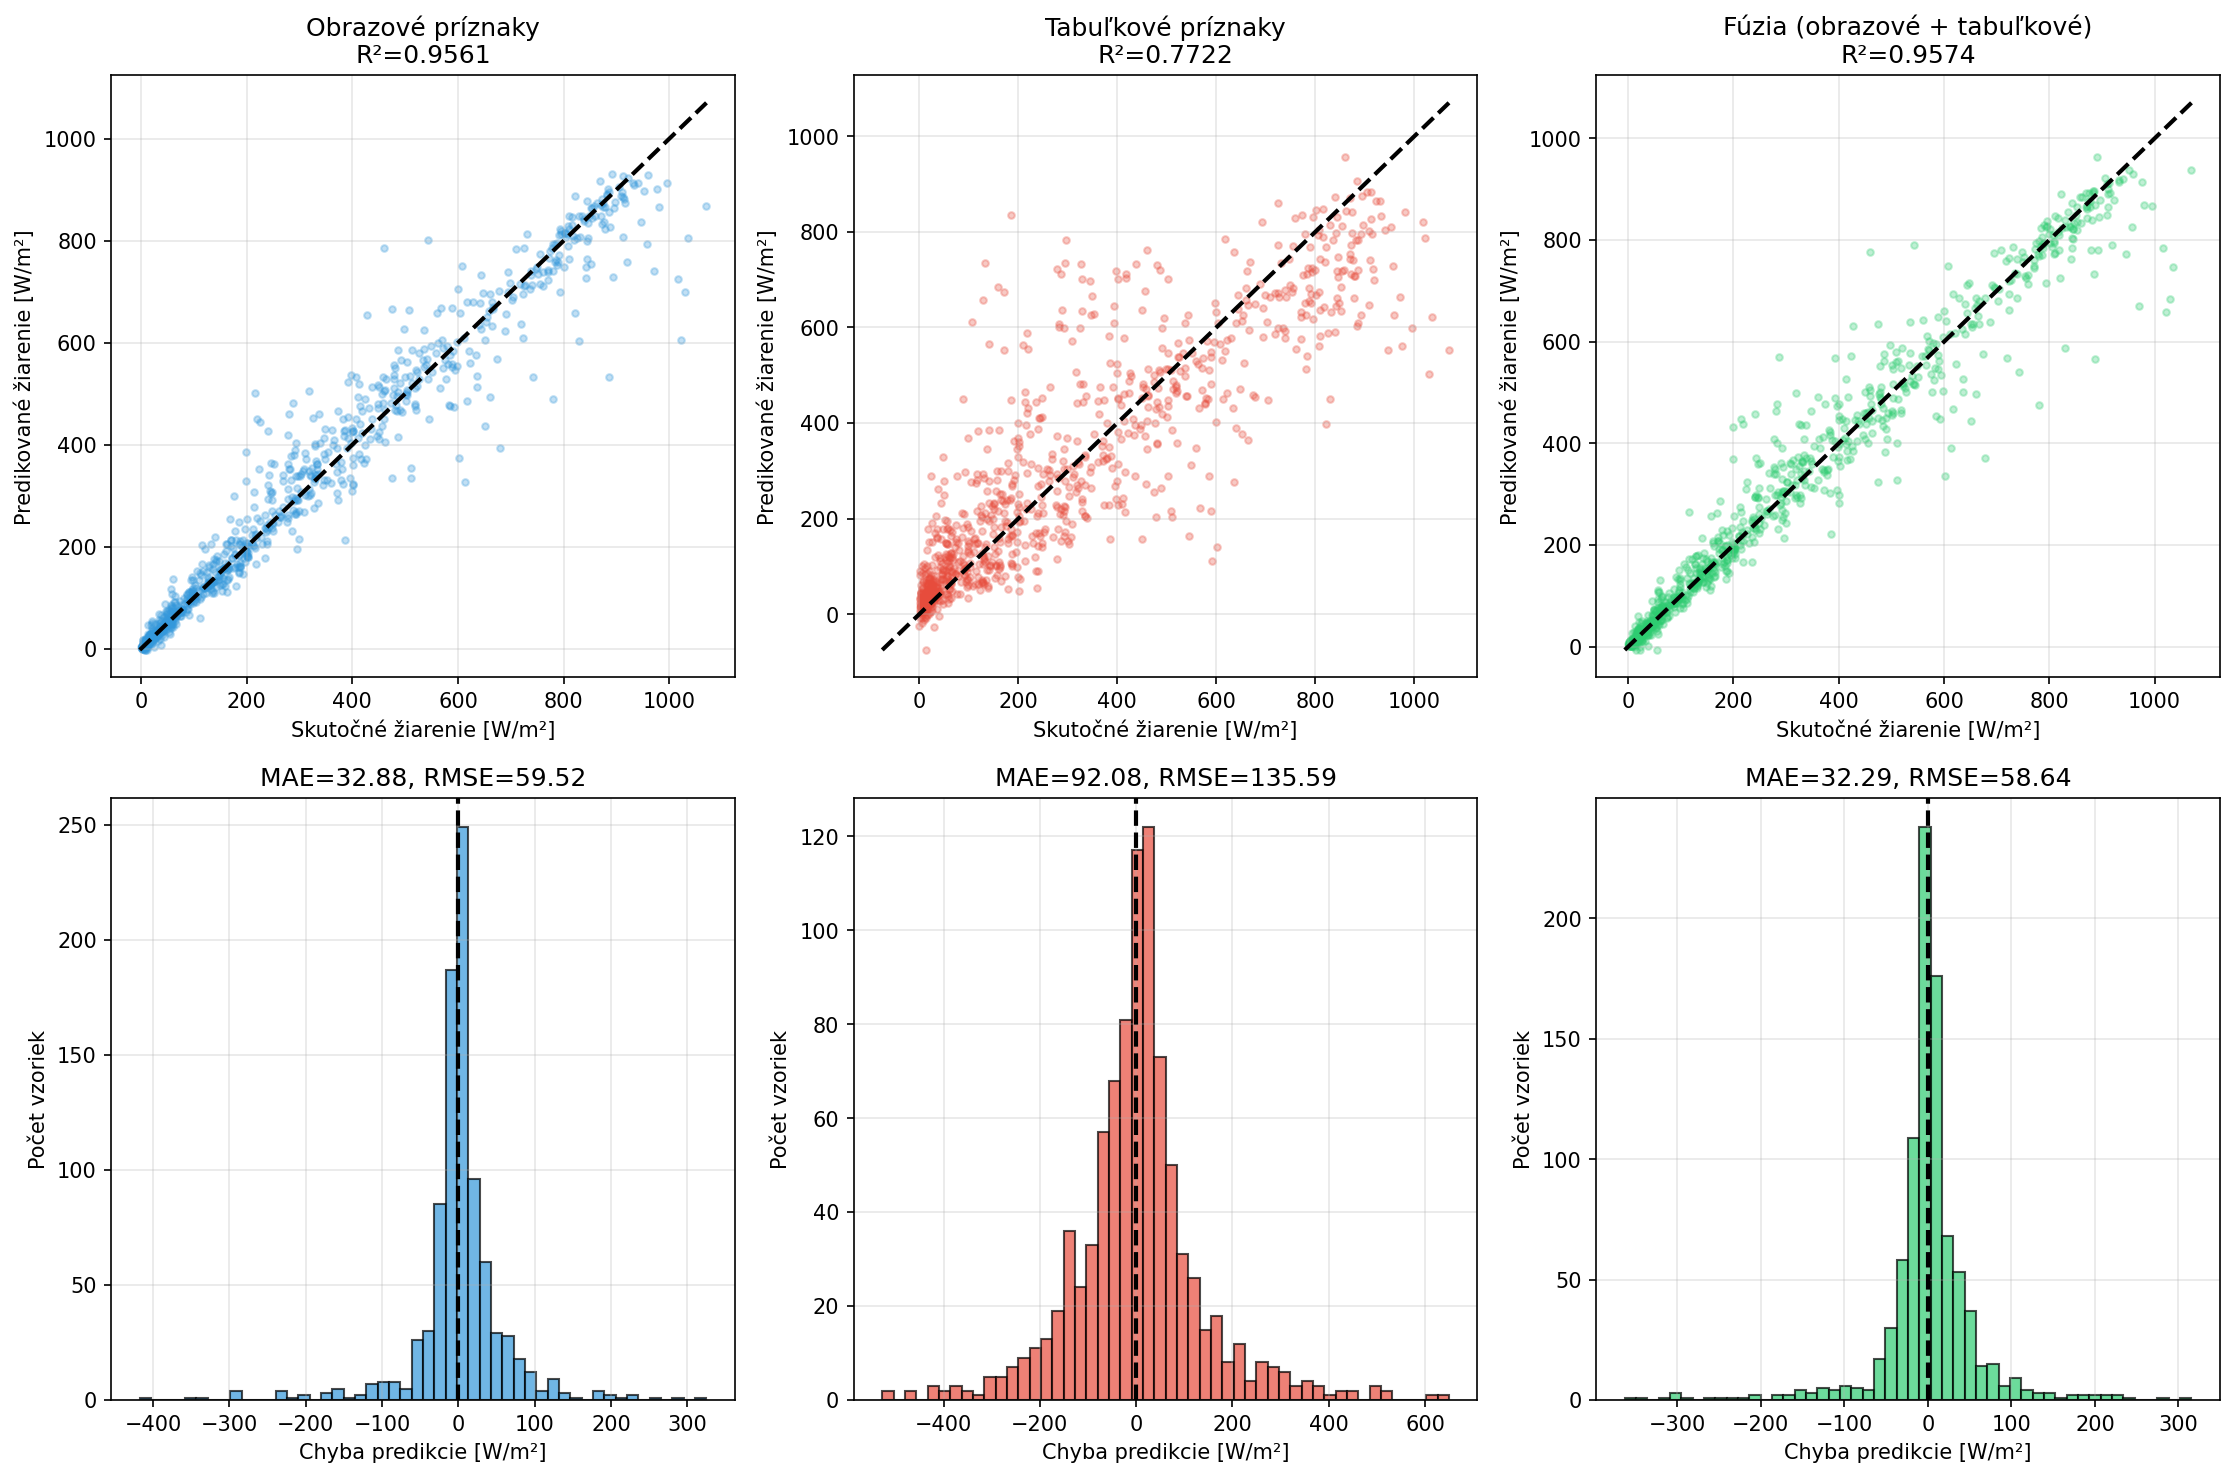
\includegraphics[width=1.1\textwidth]{../figures/bonus_fusion_comparison.png}
    \caption{Porovnanie modelov: obrazové vs. tabuľkové vs. fúzia}
    \label{fig:fusion_comparison}
\end{figure}

\clearpage

\begin{figure}[H]
    \centering
    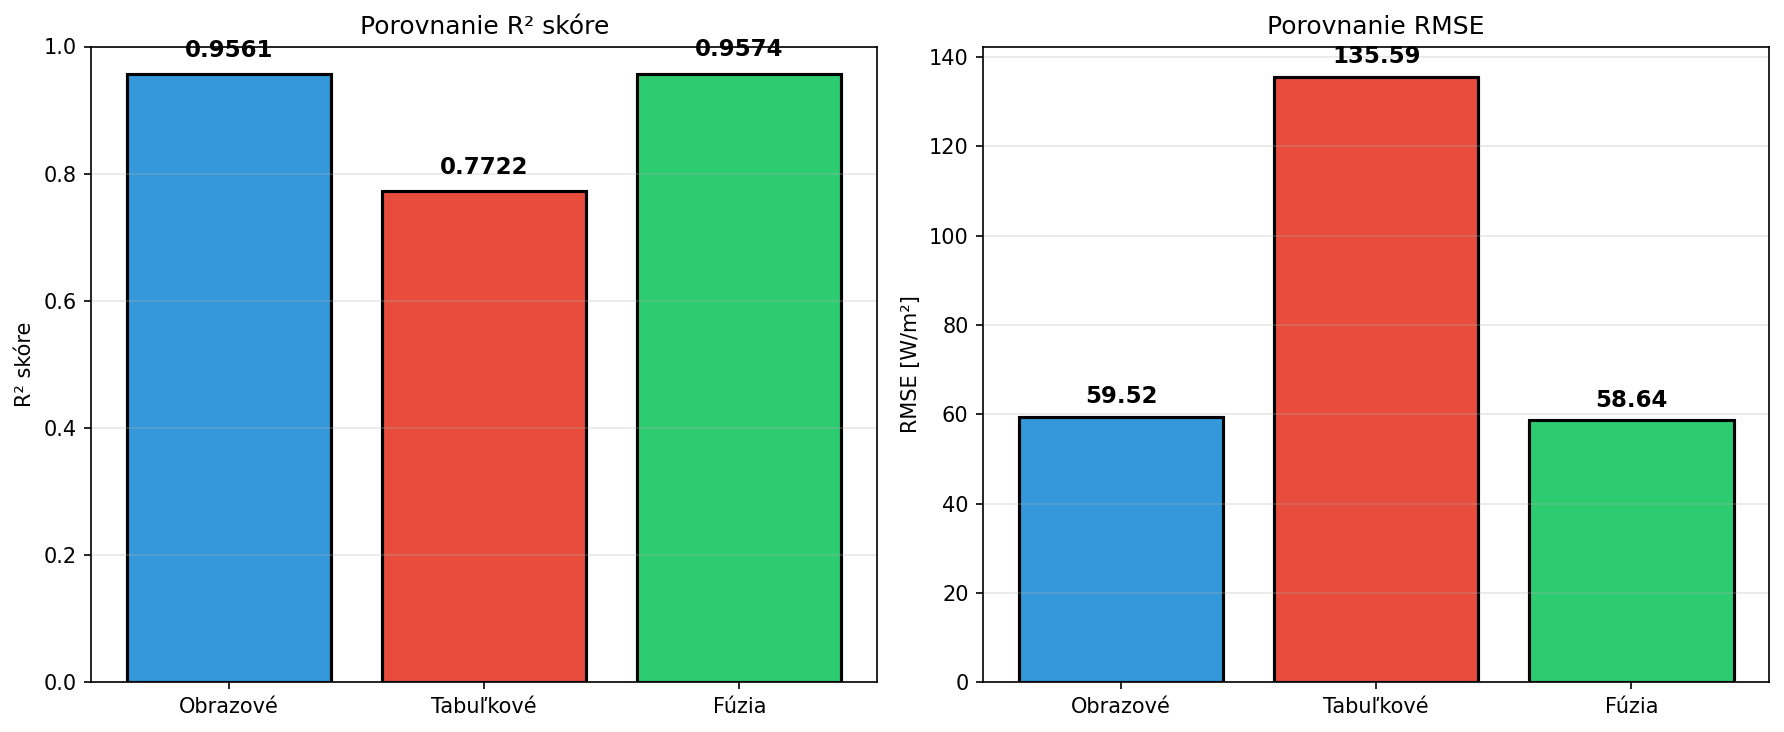
\includegraphics[width=1.1\textwidth]{../figures/bonus_fusion_metrics.png}
    \caption{Porovnanie metrík R² a~RMSE}
    \label{fig:fusion_metrics}
\end{figure}

\begin{figure}[H]
    \centering
    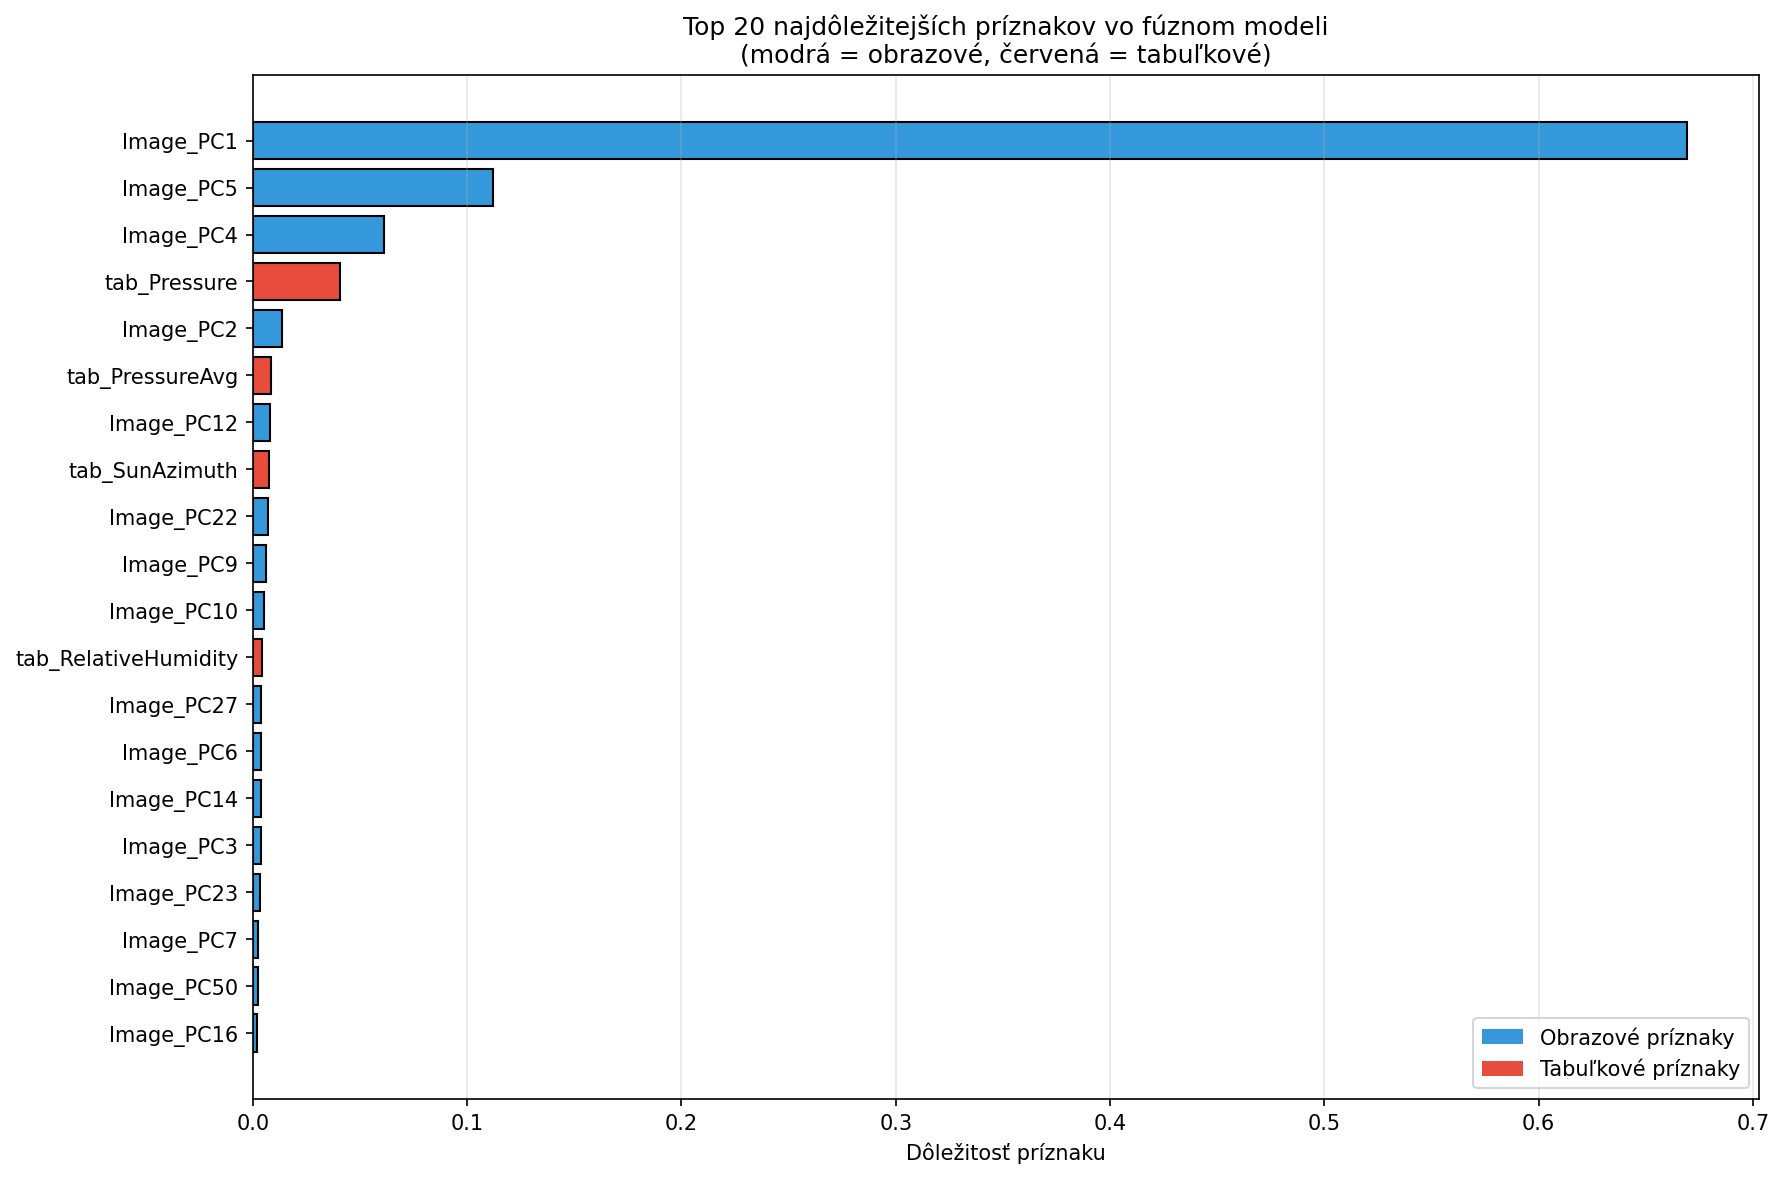
\includegraphics[width=1.1\textwidth]{../figures/bonus_fusion_feature_importance.png}
    \caption{Dôležitosť príznakov vo fúznom modeli}
    \label{fig:feature_importance}
\end{figure}

\textbf{Zistenie:} Fúzia obrazových a~tabuľkových príznakov prináša mierne zlepšenie oproti samotným obrazovým príznakom.

\clearpage

\section{Záver}

\subsection{Zhrnutie výsledkov}

Splnené tri časti zadania:

\begin{enumerate}
    \item \textbf{Exploračná dátová analýza}
    \begin{itemize}
        \item Analýza 6~007 vzoriek zo 4 mesiacov
        \item Vizualizácia distribúcií a~korelácií
        \item Rozdelenie dát 70/15/15
    \end{itemize}
    
    \item \textbf{Konvolučné neurónové siete}
    \begin{itemize}
        \item 5 konfigurácií s~rôznymi hyperparametrami
        \item Najlepší model: R² = 0.9744, RMSE = 45.43 W/m²
        \item Žiadny významný overfitting
    \end{itemize}
    
    \item \textbf{Transfer Learning a~zhlukovanie}
    \begin{itemize}
        \item Extrakcia príznakov pomocou MobileNetV2
        \item 7 zhlukov identifikovaných K-Means
        \item Stacking Ensemble: R² = 0.9601
    \end{itemize}
\end{enumerate}

\subsection{Finálne porovnanie modelov}

\begin{table}[H]
\centering
\begin{tabular}{lrrl}
\toprule
\textbf{Model} & \textbf{Test R²} & \textbf{Test RMSE} & \textbf{Poznámka} \\
\midrule
CNN (Konfig. 5) & 0.9744 & 45.43 & Najlepší výkon \\
Transfer Learning & 0.9601 & 56.73 & MobileNetV2 + Stacking \\
Fúzia (bonus) & 0.9574 & 58.64 & Obrazové + tabuľkové \\
\bottomrule
\end{tabular}
\caption{Finálne porovnanie všetkých modelov}
\end{table}

\textbf{Najlepší celkový model:} CNN Konfigurácia 5 (Širšia sieť)

\clearpage

\section*{Použitie nástrojov umelej inteligencie}

Pri vypracovaní zadania som využil nasledujúce AI nástroje ako podporné prostriedky:
\begin{itemize}
    \item \textbf{Google Gemini 3 Pro (2025):} Využitý na odborné konzultácie a na pomoc so štylistikou a formuláciou odborného textu.
\end{itemize}
\begin{itemize}
    \item \textbf{Claude Opus 4.5 (2025):} Konzultácie pri návrhu architektúry CNN, brainstorming prístupov k~transfer learning a~diskusia o~vhodných metódach zhlukovania.
\end{itemize}

\section*{Zdroje}

\begin{enumerate}
    \item PyTorch Documentation. (2025). \textit{Convolutional Neural Networks}. \\
    \url{https://pytorch.org/tutorials/beginner/blitz/cifar10_tutorial.html}
    
    \item Intel Corporation. (2025). \textit{Intel Extension for PyTorch - Installation Guide}. \\
    \url{https://pytorch-extension.intel.com/installation}
    
    \item scikit-learn Documentation. (2025). \textit{Stacking Regressor}. \\
    \url{https://scikit-learn.org/stable/modules/ensemble.html#stacked-generalization}
    
    \item TorchVision Documentation. (2025). \textit{MobileNetV2}. \\
    \url{https://pytorch.org/vision/stable/models/mobilenetv2.html}
    
    \item van der Maaten, L., \& Hinton, G. (2008). \textit{Visualizing Data using t-SNE}. \\
    \url{https://www.jmlr.org/papers/v9/vandermaaten08a.html}
\end{enumerate}

\end{document}
